\documentclass[twoside]{book}

% Packages required by doxygen
\usepackage{fixltx2e}
\usepackage{calc}
\usepackage{doxygen}
\usepackage[export]{adjustbox} % also loads graphicx
\usepackage{graphicx}
\usepackage[utf8]{inputenc}
\usepackage{makeidx}
\usepackage{multicol}
\usepackage{multirow}
\PassOptionsToPackage{warn}{textcomp}
\usepackage{textcomp}
\usepackage[nointegrals]{wasysym}
\usepackage[table]{xcolor}

% Font selection
\usepackage[T1]{fontenc}
\usepackage[scaled=.90]{helvet}
\usepackage{courier}
\usepackage{amssymb}
\usepackage{sectsty}
\renewcommand{\familydefault}{\sfdefault}
\allsectionsfont{%
  \fontseries{bc}\selectfont%
  \color{darkgray}%
}
\renewcommand{\DoxyLabelFont}{%
  \fontseries{bc}\selectfont%
  \color{darkgray}%
}
\newcommand{\+}{\discretionary{\mbox{\scriptsize$\hookleftarrow$}}{}{}}

% Page & text layout
\usepackage{geometry}
\geometry{%
  a4paper,%
  top=2.5cm,%
  bottom=2.5cm,%
  left=2.5cm,%
  right=2.5cm%
}
\tolerance=750
\hfuzz=15pt
\hbadness=750
\setlength{\emergencystretch}{15pt}
\setlength{\parindent}{0cm}
\setlength{\parskip}{3ex plus 2ex minus 2ex}
\makeatletter
\renewcommand{\paragraph}{%
  \@startsection{paragraph}{4}{0ex}{-1.0ex}{1.0ex}{%
    \normalfont\normalsize\bfseries\SS@parafont%
  }%
}
\renewcommand{\subparagraph}{%
  \@startsection{subparagraph}{5}{0ex}{-1.0ex}{1.0ex}{%
    \normalfont\normalsize\bfseries\SS@subparafont%
  }%
}
\makeatother

% Headers & footers
\usepackage{fancyhdr}
\pagestyle{fancyplain}
\fancyhead[LE]{\fancyplain{}{\bfseries\thepage}}
\fancyhead[CE]{\fancyplain{}{}}
\fancyhead[RE]{\fancyplain{}{\bfseries\leftmark}}
\fancyhead[LO]{\fancyplain{}{\bfseries\rightmark}}
\fancyhead[CO]{\fancyplain{}{}}
\fancyhead[RO]{\fancyplain{}{\bfseries\thepage}}
\fancyfoot[LE]{\fancyplain{}{}}
\fancyfoot[CE]{\fancyplain{}{}}
\fancyfoot[RE]{\fancyplain{}{\bfseries\scriptsize Generated by Doxygen }}
\fancyfoot[LO]{\fancyplain{}{\bfseries\scriptsize Generated by Doxygen }}
\fancyfoot[CO]{\fancyplain{}{}}
\fancyfoot[RO]{\fancyplain{}{}}
\renewcommand{\footrulewidth}{0.4pt}
\renewcommand{\chaptermark}[1]{%
  \markboth{#1}{}%
}
\renewcommand{\sectionmark}[1]{%
  \markright{\thesection\ #1}%
}

% Indices & bibliography
\usepackage{natbib}
\usepackage[titles]{tocloft}
\setcounter{tocdepth}{3}
\setcounter{secnumdepth}{5}
\makeindex

% Hyperlinks (required, but should be loaded last)
\usepackage{ifpdf}
\ifpdf
  \usepackage[pdftex,pagebackref=true]{hyperref}
\else
  \usepackage[ps2pdf,pagebackref=true]{hyperref}
\fi
\hypersetup{%
  colorlinks=true,%
  linkcolor=blue,%
  citecolor=blue,%
  unicode%
}

% Custom commands
\newcommand{\clearemptydoublepage}{%
  \newpage{\pagestyle{empty}\cleardoublepage}%
}

\usepackage{caption}
\captionsetup{labelsep=space,justification=centering,font={bf},singlelinecheck=off,skip=4pt,position=top}

%===== C O N T E N T S =====

\begin{document}

% Titlepage & ToC
\hypersetup{pageanchor=false,
             bookmarksnumbered=true,
             pdfencoding=unicode
            }
\pagenumbering{roman}
\begin{titlepage}
\vspace*{7cm}
\begin{center}%
{\Large u5e }\\
\vspace*{1cm}
{\large Generated by Doxygen 1.8.11}\\
\end{center}
\end{titlepage}
\clearemptydoublepage
\tableofcontents
\clearemptydoublepage
\pagenumbering{arabic}
\hypersetup{pageanchor=true}

%--- Begin generated contents ---
\chapter{u5e}
\label{index}\hypertarget{index}{}Unicode Text C++ library -- fork me on github\+: \href{https://github.com/ruoso/u5e}{\tt https\+://github.\+com/ruoso/u5e}

\section*{What is this library?}

This library provides support for Unicode Text, as specified by the Unicode Standard.

These are the problems that this library intends to solve (links for examples)\+:


\begin{DoxyItemize}
\item Iterating and truncating on correct boundaries for\+:
\begin{DoxyItemize}
\item codepoints -\/ \href{simple_iteration.html}{\tt iterate}, \href{smallest_code.html}{\tt over const char$\ast$}, \href{truncate_on_codepoint.html}{\tt truncate}.
\item graphemes -\/ \href{grapheme_iteration.html}{\tt iterate}, \href{truncate_on_grapheme.html}{\tt truncate}.
\item words
\item sentences
\end{DoxyItemize}
\item Normalization
\begin{DoxyItemize}
\item Normalization Form D -\/ \href{normalization_form_d.html}{\tt in utf8}, \href{normalization_form_d_utf32.html}{\tt in utf32}
\item Normalization Form C -\/ \href{normalization_form_c.html}{\tt in utf8}, \href{normalization_form_c_utf32.html}{\tt in utf32}
\item Normalization Form KD -\/ \href{normalization_form_kd.html}{\tt in utf8}, \href{normalization_form_kd_utf32.html}{\tt in utf32}
\item Normalization Form KC -\/ \href{normalization_form_kc.html}{\tt in utf8}, \href{normalization_form_kc_utf32.html}{\tt in utf32}
\end{DoxyItemize}
\item Explicitly Localized and Explicitly Non-\/localized support for\+:
\begin{DoxyItemize}
\item Comparison
\item Sorting
\item Case Folding
\item Search Folding (folded to \textquotesingle{}base character\textquotesingle{})
\item Tokenizing
\end{DoxyItemize}
\end{DoxyItemize}

\section*{Why?}

Properly supporting international text is one of these problems that you either think is very easy because you never had to deal with internationalized text, or you give up on it because you think no one can support Unicode correctly. This library is an attempt to provide a simple reusable set of interfaces to deal with international text.

\section*{Why not just use the icu library?}

The first reason for me to consider this was that the icu library is much more complex than what\textquotesingle{}s required for supporting text. I\+CU also supports the full localization definitions of the Unicode C\+L\+DR, which makes its support surface much larger than would be required for simply handling text.

Secondly, the icu library forces the internal representation of the text to always be in a particular encoding (U\+T\+F16). I believe that this is an unecessary constraint, and one of the points of this library is to make the encoding pluggable without requiring different A\+P\+Is or explicit conversions.

\section*{Some important conversations}

\subsection*{A note on dynamic encodings}

While it is technically possible to operate on text with a dynamically assigned encoding, I honestly believe the use case for that is more academic than anything else.

Your application should have one internal encoding and all text should be converted on the borders of the application to whatever makes the most sense for your application.

For instance, if you\textquotesingle{}re dealing with mostly 7-\/bit A\+S\+C\+II text with the ocasional exception (such as most latin languages), U\+T\+F8 is definitely the most efficient usage of memory, and will promote the best cache locality.

If, on the other hand, the application is expected to deal with mostly non-\/latin text, U\+T\+F16 is believed to result in the smallest memory usage.

But if you don\textquotesingle{}t quite care about memory usage and you have a stronger requirement for being able to do more efficient random access on the text, U\+T\+F32 with native endianess will make the most sense.

It is, of course, technically feasible to have encodings that make decisions at run time, but the cost of that runtime decision will be paid over and over in the life-\/cycle of that object.

For that reason, it is much more intelligent to convert the text to one of U\+T\+F8, U\+T\+F16 with native endianess or U\+T\+F32 with native endianess at the border of your application. I cannot see a rason to support any other encoding as the basis for operating on the text, any other encoding may be considered a serialization format to be converted to and from in the borders of your application.

Note that since the encoding is pluggable, it would be possible for a third-\/party to contribute support for dynamic encodings.

\subsection*{A note on endianess}

The unicode standard defines U\+T\+F16\+BE and U\+T\+F16\+LE, as well as U\+T\+F32\+BE and U\+T\+F32\+LE. The bare \char`\"{}\+U\+T\+F16\char`\"{} and \char`\"{}\+U\+T\+F32\char`\"{} encodings are actually runtime-\/defined according to Byte-\/\+Order-\/\+Marker (B\+OM), the default, in the absense of a B\+OM is Big-\/\+Endian, accorting to the standard -- utf8 is always little endian, and B\+OM characters in utf8 are not relevant.

This library introduces the terms U\+T\+F16\+NE and U\+T\+F32\+NE. Those are not encodings, but rather architecture-\/specific runtime types that will either be the BE or the LE variants depending on the machine that runs it. Whenever you are using the U\+T\+F16\+NE and U\+T\+F32\+NE types, you are expected to appropriately convert the incoming texts to the correct native encoding on the borders of your application.

\subsection*{A note on legacy encodings}

This library will not support converting to and from legacy encodings as well as operating on them. You are expected to perform the convertions at the borders of your application.

Note that since the encoding is pluggable, it would be possible for a third-\/party to contribute support for native encodings.

\subsection*{A note on bound checks}

U\+T\+F8 and U\+T\+F16 introduce a new possible type of overflow and underflow. If you are trying to iterate forward, the first octet in U\+T\+F8 -- or the first 16bit in U\+T\+F16 -- may tell you to look for more characters than what fits in the rest of the buffer. Likewise, if you\textquotesingle{}re iterating backwards, the first octet of your utf8 text -- or 16bits in utf16 -- may tell you that you need to look further back, underflowing the buffer.

There are two possible ways to handle this, the first is to make the bounds check pervasively in the code. This means that the entire A\+PI needs to be more complicated because every operation now needs to know where the string ends, not to mention that the additional checks will have a compounding runtime cost.

The alternative, which is what this library implements, is to validate the strings in the borders of your application, whenever you receive a text from the outside, you need to check for correctness on the start and end of your text.

This library will offer a utility function to verify the correctness of the string, and optionally forcing the replacement of the invalid utf8 and utf16 sequences by replacement characters.

\section*{This library will not cover}

These are the problems that are explicitly outside of the scope of this library. They can, and most likely should, be solved in libraries built on top of \hyperlink{namespaceu5e}{u5e}.


\begin{DoxyItemize}
\item Rendering
\item Font sizes
\item Word wrapping
\item Text presentation order (L\+TR vs R\+TL)
\item Number and Date formatting and parsing
\item Regular Expressions
\item Streaming, specifically partial reads and writes
\end{DoxyItemize}

\section*{What are the guiding principles?}

\subsection*{No \char`\"{}natural\char`\"{} unit}

There is no default unit. Most of the confusion around unicode is derived from the misconceptions on how to iterate over text and how to count and measure it. This libray defines and uses the following units\+:


\begin{DoxyEnumerate}
\item native size\+: This measure the size of the text in its in-\/memory representation. It is not necessarily a number of bytes, but it\textquotesingle{}s rather a variable size depending on the encoding and on the architecture where the code is running\+: for instance, U\+T\+F8 always uses octets as the encoding unit, however U\+T\+F32 may either use a 32 bit int, if the endianess is the same, or it may still be forced to use octets if it\textquotesingle{}s the wrong endianess. The size in bytes is an implementation detail that is architecture-\/specific and can be measured using operators like sizeof().
\item codepoint\+: The unicode standard calls this \char`\"{}character\char`\"{}, but the oveloading of this term is definitely one of the main sources of confusion around the unicode standard, therefore, in this library we just do not ever use the term \char`\"{}character\char`\"{}, and prefer the more precise term \char`\"{}codepoint\char`\"{}, which represents an encoded unicode entity, which is usually represented as U+\+D\+E\+A\+D\+B\+E\+EF.
\item grapheme\+: The grapheme is the unit of rendering, also referenced in the standard as \char`\"{}grapheme cluster\char`\"{} or \char`\"{}user perceived
   character\char`\"{}. It represents a sequence of one or more codepoints that represent a single graphical symbol, previous versions of the unicode standard had a simple rule of \char`\"{}base character\char`\"{} and \char`\"{}combining characters\char`\"{}, but more recent versions of the standard support more complex definitions for grapheme cluster boundaries.
\item word\+: A word is a set of graphemes that form a unit, it can be as simple as \char`\"{}two words\char`\"{} for english, but it requires the use of the unicode database for full internationalization support.
\item sentence\+: A collection of words. There is a property of codepoints in the unicode database that specifies if a given character is a sentence separator or not.
\end{DoxyEnumerate}

\subsection*{Handling of text requires intermediate buffers}

There is no sane way to handle text directly on streams, see \hyperlink{md__home_ruoso_devel_u5e_StreamVsIterators}{Streams versus Iterators} for a longer discussion.

\subsection*{Number and Date format is outside of the scope}

The coupling of number and date format to streams is a major source of ambiguity in the standard library, see \hyperlink{md__home_ruoso_devel_u5e_StreamVsFormat}{Streams versus Format} for a longer discussion.

\section*{The different aspects of Text}

In order to allow maximum reusability of the code, each aspect of the text is going to be expressed in this library as a concept. Different traits will implement that concept in different ways in order to at the same time allow room for optimizations. For instance, U\+T\+F32 with native endianess will be able to use the native integer type, while U\+T\+F32 with the foreign endianess will need to use four octets and will need to do the byte-\/swapping at runtime for most operations.

The usage of traits for this also gives us transparent type-\/safety. Such that we can statically evaluate if you are incorrectly mixing texts of different encodings, which is the most common form of mistake when handling internationalized text.

\subsection*{Encoding}

The encoding concept will provide that basic interface from the in-\/memory representation to iteration and access of codepoints.

\subsection*{Normalization Form}

Normalization is what allows equivalent sequences of characters to be treated as being the same. By making the normalization a trait of the text, we allow the implicit re-\/normalization when dealing with denormalized text, at te same time that it gives room for important optimizations when two different texts have the same normalization form.

\subsection*{Locale tailoring}

The unicode standard has several features that are coupled with the tailoring to specific locales, this will also be applicable to different features. Making this into a trait allows to selectively disable the tailoring for application where the speed gain from not supporting this is more important than the use cases where such support is a requirement. Making this into a trait even allows optimizing away the storage required for storing the language of the text, or if an application needs optimization for the tailoring for a single language, it could be implemented directly as code and avoid any runtime language queries. 
\chapter{Example\+: Iterate over graphemes in utf8 text}
\label{grapheme_iteration}
\hypertarget{grapheme_iteration}{}
This example covers the basic usage of iterating over utf8 text grapheme by grapheme.


\begin{DoxyCode}

\textcolor{preprocessor}{#include <experimental/string\_view>}
\textcolor{preprocessor}{#include <u5e/utf8\_string\_view.hpp>}
\textcolor{preprocessor}{#include <u5e/utf8\_string\_view\_grapheme.hpp>}
\textcolor{preprocessor}{#include <u5e/utf8\_string\_view\_grapheme\_iterator.hpp>}
\textcolor{preprocessor}{#include <stdio.h>}

\textcolor{keyword}{using} std::experimental::string\_view;
\textcolor{keyword}{using} \hyperlink{namespaceu5e_af5abb9026a8b93e2aadd01ee514208d3}{u5e::utf8\_string\_view};
\textcolor{keyword}{using} \hyperlink{namespaceu5e_a3255333e6ec6b7d9fd55a3937b445a9e}{u5e::utf8\_string\_view\_grapheme};
\textcolor{keyword}{using} \hyperlink{namespaceu5e_a3e36b87941b75a409fff1cae69b5bdb0}{u5e::utf8\_string\_view\_grapheme\_iterator};

\textcolor{keywordtype}{int} main(\textcolor{keywordtype}{int} argc, \textcolor{keywordtype}{char} **argv) \{

  \textcolor{comment}{// for each argument}
  \textcolor{keywordflow}{for} (\textcolor{keywordtype}{int} i = 1; i < argc; i++) \{

    \textcolor{comment}{// get a utf8\_string\_view}
    \hyperlink{namespaceu5e_af5abb9026a8b93e2aadd01ee514208d3}{utf8\_string\_view} p(argv[i]);

    \textcolor{comment}{// get the grapheme iterator from that}
    \textcolor{comment}{// Iterate grapheme by grapheme}
    \textcolor{keywordflow}{for} (utf8\_string\_view\_grapheme\_iterator gi = p.grapheme\_begin();
         gi != p.grapheme\_end(); gi++) \{
      \hyperlink{namespaceu5e_a3255333e6ec6b7d9fd55a3937b445a9e}{utf8\_string\_view\_grapheme} g = *gi;
      printf(\textcolor{stringliteral}{"["});

      \textcolor{comment}{// then iterate the codepoints inside that grapheme}
      \textcolor{keywordflow}{for} (utf8\_string\_view::const\_iterator it = g.codepoint\_begin();
           it != g.codepoint\_end(); it++ ) \{
        \textcolor{comment}{// the value dereferenced is the codepoint, not octets even if}
        \textcolor{comment}{// the original text had "wide" chars.}
        printf(\textcolor{stringliteral}{" U+%06llx"}, (\textcolor{keywordtype}{long} \textcolor{keywordtype}{long} \textcolor{keywordtype}{unsigned} \textcolor{keywordtype}{int})*it);
      \}

      printf(\textcolor{stringliteral}{" ]"});
    \}

    printf(\textcolor{stringliteral}{"\(\backslash\)n"});
  \}
  \textcolor{keywordflow}{return} 0;
\}
\end{DoxyCode}
 
\chapter{Example\+: Normalize a utf8 string in form C}
\label{normalization_form_c}
\hypertarget{normalization_form_c}{}
This example covers the usage of \hyperlink{namespaceu5e_a300b77046593bf5484867461ac65cb88}{u5e\+::filter} with \hyperlink{namespaceu5e_a683f83d363d3e0fbfa6417e4b4b44123}{u5e\+::normalization\+\_\+form\+\_\+c} in order to normalize a utf8 string.


\begin{DoxyCode}

\textcolor{preprocessor}{#include <u5e/utf8\_string.hpp>}
\textcolor{preprocessor}{#include <u5e/filter.hpp>}
\textcolor{preprocessor}{#include <u5e/normalization\_form\_c.hpp>}
\textcolor{preprocessor}{#include <stdio.h>}

\textcolor{keywordtype}{int} main(\textcolor{keywordtype}{int} argc, \textcolor{keywordtype}{char} **argv) \{

  \textcolor{comment}{// for each argument}
  \textcolor{keywordflow}{for} (\textcolor{keywordtype}{int} i = 1; i < argc; i++) \{

    \textcolor{comment}{// get a utf8\_string\_view}
    \hyperlink{classu5e_1_1utf8__string}{u5e::utf8\_string} input(argv[i]);
    \hyperlink{classu5e_1_1utf8__string}{u5e::utf8\_string} output;
    \hyperlink{namespaceu5e_a300b77046593bf5484867461ac65cb88}{u5e::filter}(input.grapheme\_begin(), input.grapheme\_end(), output,
                u5e::normalization\_form\_c<u5e::utf8\_string>);
    
    \textcolor{comment}{// print out the codepoints}
    \textcolor{keywordflow}{for} (\hyperlink{classu5e_1_1basic__encodedstring_a249da58e8bad9c91fab547516f90c60d}{u5e::utf8\_string::const\_iterator} it = output.codepoint\_cbegin();
         it != output.codepoint\_cend(); it++ ) \{
      \textcolor{comment}{// the value dereferenced is the codepoint, not octets even if}
      \textcolor{comment}{// the original text had "wide" chars.}
      printf(\textcolor{stringliteral}{" U+%06llx"}, (\textcolor{keywordtype}{long} \textcolor{keywordtype}{long} \textcolor{keywordtype}{unsigned} \textcolor{keywordtype}{int})*it);
    \}

    printf(\textcolor{stringliteral}{"\(\backslash\)n"});
  \}
  \textcolor{keywordflow}{return} 0;
\}
\end{DoxyCode}
 
\chapter{Example\+: Normalize a utf32 string in form C}
\label{normalization_form_c_utf32}
\hypertarget{normalization_form_c_utf32}{}
This example covers the usage of \hyperlink{namespaceu5e_a300b77046593bf5484867461ac65cb88}{u5e\+::filter} with \hyperlink{namespaceu5e_a683f83d363d3e0fbfa6417e4b4b44123}{u5e\+::normalization\+\_\+form\+\_\+c} in order to normalize a utf32 string in the native endianess.


\begin{DoxyCode}

\textcolor{preprocessor}{#include <u5e/utf32ne\_string.hpp>}
\textcolor{preprocessor}{#include <u5e/filter.hpp>}
\textcolor{preprocessor}{#include <u5e/normalization\_form\_c.hpp>}
\textcolor{preprocessor}{#include <stdio.h>}

\textcolor{keywordtype}{int} main(\textcolor{keywordtype}{int} argc, \textcolor{keywordtype}{char} **argv) \{

  \hyperlink{classu5e_1_1utf32ne__string}{u5e::utf32ne\_string} input(\{ 0xC4, 0xFB03, \textcolor{charliteral}{'n'} \});
  \hyperlink{classu5e_1_1utf32ne__string}{u5e::utf32ne\_string} output;
  \hyperlink{namespaceu5e_a300b77046593bf5484867461ac65cb88}{u5e::filter}(input.grapheme\_begin(), input.grapheme\_end(), output,
              u5e::normalization\_form\_c<u5e::utf32ne\_string>);
    
  \textcolor{comment}{// print out the codepoints}
  \textcolor{keywordflow}{for} (\hyperlink{classu5e_1_1basic__encodedstring_a249da58e8bad9c91fab547516f90c60d}{u5e::utf32ne\_string::const\_iterator} it = output.codepoint\_cbegin(
      );
       it != output.codepoint\_cend(); it++ ) \{
    printf(\textcolor{stringliteral}{" U+%06llx"}, (\textcolor{keywordtype}{long} \textcolor{keywordtype}{long} \textcolor{keywordtype}{unsigned} \textcolor{keywordtype}{int})*it);
  \}

  \textcolor{keywordflow}{return} 0;
\}
\end{DoxyCode}
 
\chapter{Example\+: Normalize a utf8 string in form D}
\label{normalization_form_d}
\hypertarget{normalization_form_d}{}
This example covers the usage of \hyperlink{namespaceu5e_a300b77046593bf5484867461ac65cb88}{u5e\+::filter} with \hyperlink{namespaceu5e_a1fe914ecfbcbfd5630b6c38c696b868f}{u5e\+::normalization\+\_\+form\+\_\+d} in order to normalize a utf8 string.


\begin{DoxyCode}

\textcolor{preprocessor}{#include <u5e/utf8\_string.hpp>}
\textcolor{preprocessor}{#include <u5e/filter.hpp>}
\textcolor{preprocessor}{#include <u5e/normalization\_form\_d.hpp>}
\textcolor{preprocessor}{#include <stdio.h>}

\textcolor{keywordtype}{int} main(\textcolor{keywordtype}{int} argc, \textcolor{keywordtype}{char} **argv) \{

  \textcolor{comment}{// for each argument}
  \textcolor{keywordflow}{for} (\textcolor{keywordtype}{int} i = 1; i < argc; i++) \{

    \textcolor{comment}{// get a utf8\_string\_view}
    \hyperlink{classu5e_1_1utf8__string}{u5e::utf8\_string} input(argv[i]);
    \hyperlink{classu5e_1_1utf8__string}{u5e::utf8\_string} output;
    \hyperlink{namespaceu5e_a300b77046593bf5484867461ac65cb88}{u5e::filter}(input.grapheme\_begin(), input.grapheme\_end(), output,
                u5e::normalization\_form\_d<u5e::utf8\_string>);
    
    \textcolor{comment}{// print out the codepoints}
    \textcolor{keywordflow}{for} (\hyperlink{classu5e_1_1basic__encodedstring_a249da58e8bad9c91fab547516f90c60d}{u5e::utf8\_string::const\_iterator} it = output.codepoint\_cbegin();
         it != output.codepoint\_cend(); it++ ) \{
      \textcolor{comment}{// the value dereferenced is the codepoint, not octets even if}
      \textcolor{comment}{// the original text had "wide" chars.}
      printf(\textcolor{stringliteral}{" U+%06llx"}, (\textcolor{keywordtype}{long} \textcolor{keywordtype}{long} \textcolor{keywordtype}{unsigned} \textcolor{keywordtype}{int})*it);
    \}

    printf(\textcolor{stringliteral}{"\(\backslash\)n"});
  \}
  \textcolor{keywordflow}{return} 0;
\}
\end{DoxyCode}
 
\chapter{Example\+: Normalize a utf32 string in form D}
\label{normalization_form_d_utf32}
\hypertarget{normalization_form_d_utf32}{}
This example covers the usage of \hyperlink{namespaceu5e_a300b77046593bf5484867461ac65cb88}{u5e\+::filter} with \hyperlink{namespaceu5e_a1fe914ecfbcbfd5630b6c38c696b868f}{u5e\+::normalization\+\_\+form\+\_\+d} in order to normalize a utf32 string in the native endianess.


\begin{DoxyCode}

\textcolor{preprocessor}{#include <u5e/utf32ne\_string.hpp>}
\textcolor{preprocessor}{#include <u5e/filter.hpp>}
\textcolor{preprocessor}{#include <u5e/normalization\_form\_d.hpp>}
\textcolor{preprocessor}{#include <stdio.h>}

\textcolor{keywordtype}{int} main(\textcolor{keywordtype}{int} argc, \textcolor{keywordtype}{char} **argv) \{

  \hyperlink{classu5e_1_1utf32ne__string}{u5e::utf32ne\_string} input(\{ 0xC4, 0xFB03, \textcolor{charliteral}{'n'} \});
  \hyperlink{classu5e_1_1utf32ne__string}{u5e::utf32ne\_string} output;
  \hyperlink{namespaceu5e_a300b77046593bf5484867461ac65cb88}{u5e::filter}(input.grapheme\_begin(), input.grapheme\_end(), output,
              u5e::normalization\_form\_d<u5e::utf32ne\_string>);
    
  \textcolor{comment}{// print out the codepoints}
  \textcolor{keywordflow}{for} (\hyperlink{classu5e_1_1basic__encodedstring_a249da58e8bad9c91fab547516f90c60d}{u5e::utf32ne\_string::const\_iterator} it = output.codepoint\_cbegin(
      );
       it != output.codepoint\_cend(); it++ ) \{
    printf(\textcolor{stringliteral}{" U+%06llx"}, (\textcolor{keywordtype}{long} \textcolor{keywordtype}{long} \textcolor{keywordtype}{unsigned} \textcolor{keywordtype}{int})*it);
  \}

  \textcolor{keywordflow}{return} 0;
\}
\end{DoxyCode}
 
\chapter{Example\+: Normalize a utf8 string in form C}
\label{normalization_form_kc}
\hypertarget{normalization_form_kc}{}
This example covers the usage of \hyperlink{namespaceu5e_a300b77046593bf5484867461ac65cb88}{u5e\+::filter} with \hyperlink{namespaceu5e_a67caa33a03e9b645861525fcf447c845}{u5e\+::normalization\+\_\+form\+\_\+kc} in order to normalize a utf8 string.


\begin{DoxyCode}

\textcolor{preprocessor}{#include <u5e/utf8\_string.hpp>}
\textcolor{preprocessor}{#include <u5e/filter.hpp>}
\textcolor{preprocessor}{#include <u5e/normalization\_form\_kc.hpp>}
\textcolor{preprocessor}{#include <stdio.h>}

\textcolor{keywordtype}{int} main(\textcolor{keywordtype}{int} argc, \textcolor{keywordtype}{char} **argv) \{

  \textcolor{comment}{// for each argument}
  \textcolor{keywordflow}{for} (\textcolor{keywordtype}{int} i = 1; i < argc; i++) \{

    \textcolor{comment}{// get a utf8\_string\_view}
    \hyperlink{classu5e_1_1utf8__string}{u5e::utf8\_string} input(argv[i]);
    \hyperlink{classu5e_1_1utf8__string}{u5e::utf8\_string} output;
    \hyperlink{namespaceu5e_a300b77046593bf5484867461ac65cb88}{u5e::filter}(input.grapheme\_begin(), input.grapheme\_end(), output,
                u5e::normalization\_form\_kc<u5e::utf8\_string>);
    
    \textcolor{comment}{// print out the codepoints}
    \textcolor{keywordflow}{for} (\hyperlink{classu5e_1_1basic__encodedstring_a249da58e8bad9c91fab547516f90c60d}{u5e::utf8\_string::const\_iterator} it = output.codepoint\_cbegin();
         it != output.codepoint\_cend(); it++ ) \{
      \textcolor{comment}{// the value dereferenced is the codepoint, not octets even if}
      \textcolor{comment}{// the original text had "wide" chars.}
      printf(\textcolor{stringliteral}{" U+%06llx"}, (\textcolor{keywordtype}{long} \textcolor{keywordtype}{long} \textcolor{keywordtype}{unsigned} \textcolor{keywordtype}{int})*it);
    \}

    printf(\textcolor{stringliteral}{"\(\backslash\)n"});
  \}
  \textcolor{keywordflow}{return} 0;
\}
\end{DoxyCode}
 
\chapter{Example\+: Normalize a utf32 string in form KC}
\label{normalization_form_kc_utf32}
\hypertarget{normalization_form_kc_utf32}{}
This example covers the usage of \hyperlink{namespaceu5e_a300b77046593bf5484867461ac65cb88}{u5e\+::filter} with \hyperlink{namespaceu5e_a67caa33a03e9b645861525fcf447c845}{u5e\+::normalization\+\_\+form\+\_\+kc} in order to normalize a utf32 string in the native endianess.


\begin{DoxyCode}

\textcolor{preprocessor}{#include <u5e/utf32ne\_string.hpp>}
\textcolor{preprocessor}{#include <u5e/filter.hpp>}
\textcolor{preprocessor}{#include <u5e/normalization\_form\_kc.hpp>}
\textcolor{preprocessor}{#include <stdio.h>}

\textcolor{keywordtype}{int} main(\textcolor{keywordtype}{int} argc, \textcolor{keywordtype}{char} **argv) \{

  \hyperlink{classu5e_1_1utf32ne__string}{u5e::utf32ne\_string} input(\{ 0xC4, 0xFB03, \textcolor{charliteral}{'n'} \});
  \hyperlink{classu5e_1_1utf32ne__string}{u5e::utf32ne\_string} output;
  \hyperlink{namespaceu5e_a300b77046593bf5484867461ac65cb88}{u5e::filter}(input.grapheme\_begin(), input.grapheme\_end(), output,
              u5e::normalization\_form\_kc<u5e::utf32ne\_string>);
    
  \textcolor{comment}{// print out the codepoints}
  \textcolor{keywordflow}{for} (\hyperlink{classu5e_1_1basic__encodedstring_a249da58e8bad9c91fab547516f90c60d}{u5e::utf32ne\_string::const\_iterator} it = output.codepoint\_cbegin(
      );
       it != output.codepoint\_cend(); it++ ) \{
    printf(\textcolor{stringliteral}{" U+%06llx"}, (\textcolor{keywordtype}{long} \textcolor{keywordtype}{long} \textcolor{keywordtype}{unsigned} \textcolor{keywordtype}{int})*it);
  \}

  \textcolor{keywordflow}{return} 0;
\}
\end{DoxyCode}
 
\chapter{Example\+: Normalize a utf8 string in form D}
\label{normalization_form_kd}
\hypertarget{normalization_form_kd}{}
This example covers the usage of \hyperlink{namespaceu5e_a300b77046593bf5484867461ac65cb88}{u5e\+::filter} with \hyperlink{namespaceu5e_a27fc11752025c4901b3fdb94f014af57}{u5e\+::normalization\+\_\+form\+\_\+kd} in order to normalize a utf8 string.


\begin{DoxyCode}

\textcolor{preprocessor}{#include <u5e/utf8\_string.hpp>}
\textcolor{preprocessor}{#include <u5e/filter.hpp>}
\textcolor{preprocessor}{#include <u5e/normalization\_form\_kd.hpp>}
\textcolor{preprocessor}{#include <stdio.h>}

\textcolor{keywordtype}{int} main(\textcolor{keywordtype}{int} argc, \textcolor{keywordtype}{char} **argv) \{

  \textcolor{comment}{// for each argument}
  \textcolor{keywordflow}{for} (\textcolor{keywordtype}{int} i = 1; i < argc; i++) \{

    \textcolor{comment}{// get a utf8\_string\_view}
    \hyperlink{classu5e_1_1utf8__string}{u5e::utf8\_string} input(argv[i]);
    \hyperlink{classu5e_1_1utf8__string}{u5e::utf8\_string} output;
    \hyperlink{namespaceu5e_a300b77046593bf5484867461ac65cb88}{u5e::filter}(input.grapheme\_begin(), input.grapheme\_end(), output,
                u5e::normalization\_form\_kd<u5e::utf8\_string>);
    
    \textcolor{comment}{// print out the codepoints}
    \textcolor{keywordflow}{for} (\hyperlink{classu5e_1_1basic__encodedstring_a249da58e8bad9c91fab547516f90c60d}{u5e::utf8\_string::const\_iterator} it = output.codepoint\_cbegin();
         it != output.codepoint\_cend(); it++ ) \{
      \textcolor{comment}{// the value dereferenced is the codepoint, not octets even if}
      \textcolor{comment}{// the original text had "wide" chars.}
      printf(\textcolor{stringliteral}{" U+%06llx"}, (\textcolor{keywordtype}{long} \textcolor{keywordtype}{long} \textcolor{keywordtype}{unsigned} \textcolor{keywordtype}{int})*it);
    \}

    printf(\textcolor{stringliteral}{"\(\backslash\)n"});
  \}
  \textcolor{keywordflow}{return} 0;
\}
\end{DoxyCode}
 
\chapter{Example\+: Normalize a utf32 string in form KD}
\label{normalization_form_kd_utf32}
\hypertarget{normalization_form_kd_utf32}{}
This example covers the usage of \hyperlink{namespaceu5e_a300b77046593bf5484867461ac65cb88}{u5e\+::filter} with \hyperlink{namespaceu5e_a27fc11752025c4901b3fdb94f014af57}{u5e\+::normalization\+\_\+form\+\_\+kd} in order to normalize a utf32 string in the native endianess.


\begin{DoxyCode}

\textcolor{preprocessor}{#include <u5e/utf32ne\_string.hpp>}
\textcolor{preprocessor}{#include <u5e/filter.hpp>}
\textcolor{preprocessor}{#include <u5e/normalization\_form\_kd.hpp>}
\textcolor{preprocessor}{#include <stdio.h>}

\textcolor{keywordtype}{int} main(\textcolor{keywordtype}{int} argc, \textcolor{keywordtype}{char} **argv) \{

  \hyperlink{classu5e_1_1utf32ne__string}{u5e::utf32ne\_string} input(\{ 0xC4, 0xFB03, \textcolor{charliteral}{'n'} \});
  \hyperlink{classu5e_1_1utf32ne__string}{u5e::utf32ne\_string} output;
  \hyperlink{namespaceu5e_a300b77046593bf5484867461ac65cb88}{u5e::filter}(input.grapheme\_begin(), input.grapheme\_end(), output,
              u5e::normalization\_form\_kd<u5e::utf32ne\_string>);
    
  \textcolor{comment}{// print out the codepoints}
  \textcolor{keywordflow}{for} (\hyperlink{classu5e_1_1basic__encodedstring_a249da58e8bad9c91fab547516f90c60d}{u5e::utf32ne\_string::const\_iterator} it = output.codepoint\_cbegin(
      );
       it != output.codepoint\_cend(); it++ ) \{
    printf(\textcolor{stringliteral}{" U+%06llx"}, (\textcolor{keywordtype}{long} \textcolor{keywordtype}{long} \textcolor{keywordtype}{unsigned} \textcolor{keywordtype}{int})*it);
  \}

  \textcolor{keywordflow}{return} 0;
\}
\end{DoxyCode}
 
\chapter{Example\+: Iterate over codepoints in utf8 text}
\label{simple_iteration}
\hypertarget{simple_iteration}{}
This example covers the basic usage of iterating over utf8 text codepoint by codepoint.


\begin{DoxyCode}

\textcolor{preprocessor}{#include <experimental/string\_view>}
\textcolor{preprocessor}{#include <u5e/utf8\_string\_view.hpp>}
\textcolor{preprocessor}{#include <stdio.h>}

\textcolor{keyword}{using} std::experimental::string\_view;

\textcolor{keywordtype}{int} main(\textcolor{keywordtype}{int} argc, \textcolor{keywordtype}{char} **argv) \{
  \textcolor{comment}{// for each argument}
  \textcolor{keywordflow}{for} (\textcolor{keywordtype}{int} i = 1; i < argc; i++) \{

    \textcolor{comment}{// get a string\_view}
    string\_view p(argv[i], strlen(argv[i]));

    \textcolor{comment}{// get a utf8\_string\_view::const\_iteator}
    \hyperlink{classu5e_1_1basic__encodedstring_a249da58e8bad9c91fab547516f90c60d}{u5e::utf8\_string\_view::const\_iterator} it = p.begin();

    \textcolor{comment}{// Iterate until the end}
    \textcolor{keywordflow}{while} (it != p.end()) \{

      \textcolor{comment}{// the value dereferenced is the codepoint, not octets even if}
      \textcolor{comment}{// the original text had "wide" chars.}
      printf(\textcolor{stringliteral}{" U+%06llx "}, (\textcolor{keywordtype}{long} \textcolor{keywordtype}{long} \textcolor{keywordtype}{unsigned} \textcolor{keywordtype}{int})*it++);
      
    \}
    
    printf(\textcolor{stringliteral}{"\(\backslash\)n"});
  \}
  \textcolor{keywordflow}{return} 0;
\}
\end{DoxyCode}
 
\chapter{Example\+: using utf8\+\_\+iterator with const char$\ast$}
\label{smallest_code}
\hypertarget{smallest_code}{}
This example shows that it\textquotesingle{}s possible to use the utf8 iterator with a bare const char$\ast$, even without getting a string or a string\+\_\+view.


\begin{DoxyCode}

\textcolor{preprocessor}{#include <u5e/utf8\_iterator.hpp>}
\textcolor{keywordtype}{int} main(\textcolor{keywordtype}{int} argc, \textcolor{keywordtype}{char}** argv) \{
  \textcolor{comment}{// you can instantiate utf8\_iterator even with const char*}
  \hyperlink{classu5e_1_1utf8__iterator}{u5e::utf8\_iterator<const char*>} it(argv[1]);
  \textcolor{keywordflow}{return} *it;
\}

\end{DoxyCode}
 
\chapter{Example\+: Truncate a string on codepoint boundary}
\label{truncate_on_codepoint}
\hypertarget{truncate_on_codepoint}{}
The challenge of truncating a string is that if you operate on the native level, you risk breaking a codepoint in half.

The \hyperlink{namespaceu5e}{u5e} library provides an easy way to truncate a text, starting from a target native size and finding the correct boundary.


\begin{DoxyCode}
\textcolor{preprocessor}{#include <algorithm>}
\textcolor{preprocessor}{#include <iostream>}
\textcolor{preprocessor}{#include <string>}
\textcolor{preprocessor}{#include <u5e/utf8\_string.hpp>}
\textcolor{keyword}{using} std::string;
\textcolor{keyword}{using} \hyperlink{namespaceu5e_a3814526c6ea7ca04223a8ec1b662d497}{u5e::utf8\_string};
\textcolor{keywordtype}{int} main(\textcolor{keywordtype}{int} argc, \textcolor{keywordtype}{char}** argv) \{
  \textcolor{comment}{// the original string}
  \textcolor{keywordtype}{string} str(\textcolor{stringliteral}{"Ola\(\backslash\)xCC\(\backslash\)x81!"});

  \textcolor{comment}{// we find the point on the native string where we want to truncate.}
  \textcolor{comment}{// Count 4 in octets leaves us in the middle of a codepoint}
  string::const\_iterator stri = str.cbegin();
  std::advance(stri, 4);
  
  \textcolor{comment}{// now we produce the output string truncated at where we want.}
  \textcolor{comment}{// note that this assumes that the text was already in utf8. this is}
  \textcolor{comment}{// not a conversion operator, it just makes sure the append happens}
  \textcolor{comment}{// while respecting the codepoint boundaries in the utf8 text.}
  \hyperlink{namespaceu5e_a3814526c6ea7ca04223a8ec1b662d497}{utf8\_string} output(\textcolor{stringliteral}{""});
  output.append(str.cbegin(), stri);

  std::cout << output.native\_string << std::endl;
\}
\end{DoxyCode}
 
\chapter{Example\+: Truncate a string on grapheme boundary}
\label{truncate_on_grapheme}
\hypertarget{truncate_on_grapheme}{}
The challenge of truncating a string is that if you operate on the native level, you risk breaking a codepoint in half. And even when you take the codepoint boundaries in consideration, you still risk breaking a grapheme in half.

The \hyperlink{namespaceu5e}{u5e} library provides an easy way to truncate a text, starting from a target native size and finding the correct boundary.


\begin{DoxyCode}
\textcolor{preprocessor}{#include <algorithm>}
\textcolor{preprocessor}{#include <iostream>}
\textcolor{preprocessor}{#include <string>}
\textcolor{preprocessor}{#include <u5e/utf8\_string.hpp>}
\textcolor{preprocessor}{#include <u5e/utf8\_string\_grapheme\_iterator.hpp>}
\textcolor{keyword}{using} std::string;
\textcolor{keyword}{using} \hyperlink{namespaceu5e_a3814526c6ea7ca04223a8ec1b662d497}{u5e::utf8\_string};
\textcolor{keyword}{using} \hyperlink{namespaceu5e_a74a084fc31e6af27114007a21f6f89e7}{u5e::utf8\_string\_grapheme\_iterator};
\textcolor{keywordtype}{int} main(\textcolor{keywordtype}{int} argc, \textcolor{keywordtype}{char}** argv) \{
  \textcolor{comment}{// the original string}
  \textcolor{keywordtype}{string} str(\textcolor{stringliteral}{"Ola\(\backslash\)xCC\(\backslash\)x81!"});

  \textcolor{comment}{// we find the point on the native string where we want to truncate.}
  \textcolor{comment}{// Count 4 in octets leaves us in the middle of the second codepoint}
  \textcolor{comment}{// of a grapheme.}
  string::const\_iterator stri = str.cbegin();
  std::advance(stri, 4);

  \textcolor{comment}{// We need to promote the iterators to utf8 iterators.}
  utf8\_string::const\_iterator u8b(str.begin());
  utf8\_string::const\_iterator u8e(str.end());
  utf8\_string::const\_iterator u8i(stri);

  \textcolor{comment}{// In order to work with graphemes, we need to obtain grapheme}
  \textcolor{comment}{// iterators.}
  \hyperlink{namespaceu5e_a74a084fc31e6af27114007a21f6f89e7}{utf8\_string\_grapheme\_iterator} gb(u8b, u8e);
  \hyperlink{namespaceu5e_a74a084fc31e6af27114007a21f6f89e7}{utf8\_string\_grapheme\_iterator} gi(u8b, u8e, u8i);
  
  \textcolor{comment}{// now we produce the output string truncated at where we want.}
  \textcolor{comment}{// note that this assumes that the text was already in utf8. this is}
  \textcolor{comment}{// not a conversion operator, it just makes sure the append happens}
  \textcolor{comment}{// while respecting the codepoint and grapheme boundaries in the}
  \textcolor{comment}{// utf8 text.}
  \hyperlink{namespaceu5e_a3814526c6ea7ca04223a8ec1b662d497}{utf8\_string} output(\textcolor{stringliteral}{""});
  output.append(gb, gi);

  std::cout << output.native\_string << std::endl;
\}
\end{DoxyCode}
 
\chapter{Streams versus String Formatting}
\label{md__home_ruoso_devel_u5e_StreamVsFormat}
\hypertarget{md__home_ruoso_devel_u5e_StreamVsFormat}{}
The C++ standard library provides support for localization on a level that doesn\textquotesingle{}t quite have a analogous comparison in other languages. The way in which the stream itself is made aware of locales and how the shift operator on streams has its behaviors dependant on locales is an unique design decision on how input and output operates on an application.

Localization happens in many different levels, and coupling the reading and writing to streams with that is, imho, an unecessarily heavy-\/handed decision. Specifically, most applications read and write from streams much more frequently than when interacting with the localized user interface. It is much more frequent that an application will be dealing with serialization formats and network protocols that are not locale-\/dependant, than an application will be dealing with interactive input and output that is meant to be localized.

When working in an internationalized application, it is crucial that the moments in which the locale reflects in the behavior of the application should be explicitly demarcated from the places in which the application is dealing with \char`\"{}data\char`\"{} input and output. The C++ standard library makes that harder.

\subsection*{Streams can\textquotesingle{}t quite deal with text anyway.}

See \hyperlink{md__home_ruoso_devel_u5e_StreamVsIterators}{Streams vs Iterators} for a long explanation on why streams are the wrong tools to deal with text.

\subsection*{Number and Date format must be decoupled from the stream}

I think it\textquotesingle{}s an unavoidable fact that any number and date format must be deocupled from the stream. It is really tempting to try to optimize away the intermediate state built with the output data, but I think the problems I presented demonstrate this optimization is not viable if we want to have unambiguous handling of text.

I\textquotesingle{}d also argue that this optimization is also premature, because the context in which that formatting happens is usually already in the context of building an intermediate representation anyway. It is very common, for instance, to have the actual writing of the data on the underlying channel delegated to another thread, so in most cases the intermediate value is already present anyway.

\subsection*{The syntax-\/sugar of the shift operator may still be preserved}

A Number and Date format library can easily present a similar-\/looking syntax sugar for composing those intermediate values, wit the advantage of more clearly separating the concerns of creating the formatted value and submitting that formatted value to a stream.

That will also have the advantage of eliminating the concern of partial reads and partial writes from everything that handles text formatting and parsing. 
\chapter{Streams vs Iterators}
\label{md__home_ruoso_devel_u5e_StreamVsIterators}
\hypertarget{md__home_ruoso_devel_u5e_StreamVsIterators}{}
\begin{quote}
TL;DR\+: streams only make sense when dealing with raw data, and they should always operate in the \textquotesingle{}native character size\textquotesingle{} of the underlying channel. Operating in text requires bidirectional, concurrent access, such as what iterators provide. \end{quote}


There is a tension in purpose between streams and iterators in the C++ standard library. On one hand, it seems as if the basic form of interaction with text should be through streams and the shift operator overloads. On the other hand, not everything can be represented as a stream.

The moment where this becomes the most obvious is when you are dealing with multi-\/octet encodings as well as when dealing with multi-\/codepoint graphemes. When getting the next \char`\"{}character\char`\"{} from a stream, there\textquotesingle{}s an implicit expectation that the underlying channel supports a \char`\"{}character\char`\"{} of exatly that size.

This is important because when we\textquotesingle{}re talking about underlying streams backed up by file descriptors (e.\+g.\+: sockets or files on disk), the operating system has a \char`\"{}native character size\char`\"{} by which that operation happens. On P\+O\+S\+IX systems, that \char`\"{}native character size\char`\"{} is an octet. When we\textquotesingle{}re talking about network operations, they are defined by the T\+CP and U\+DP protocols to be have the \char`\"{}native character size\char`\"{} of an octet.

The important side-\/effect of this fact is that when dealing with a stream of a given \char`\"{}native character size\char`\"{}, any \char`\"{}character type\char`\"{} bigger than that will unavoidably be subject to being truncated or split across separate read operations.

When you are writing network-\/aware code, regardless of the encoding of the data being transmitted, the size of the T\+CP packet will be measured in bytes, regardless of you having decided to use a wchar on your code. In that lies a great challenge\+:

\begin{quote}
If you try to do a non-\/blocking write of a wchar to a socket, and you only get half of it written, what do you do? \end{quote}


\paragraph*{Option 1\+: keep a local buffer of half-\/sent wchars}

This looks good at first, but when you look at how this actually reflects on the several layers of A\+PI surrounding that decision, you will quickly notice that this will fall apart. What does your abstraction return to the calling code? Your off\+\_\+t type is not a floating point, so you can\textquotesingle{}t say that you wrote half a character.

\paragraph*{Option 2\+: Block until you can actually send the whole wchar}

This would look good if the original write operation was a blocking write, but non-\/blocking writes are definitely a fundamental part of any network protocol, so blindly disabling that feature sounds unacceptable.

\subsection*{What is the alternative?}

The alternative is actually not new, and it\textquotesingle{}s actually fairly well understood by the designers of more recent languages. The requirement is that you can\textquotesingle{}t talk about \char`\"{}text\char`\"{} when dealing with any sort of serialization. Languages like python3 have addressed this as a first-\/level problem by having two distinct types for \textquotesingle{}raw data\textquotesingle{} and \textquotesingle{}text string\textquotesingle{}.

The process of converting between that \textquotesingle{}raw data\textquotesingle{} and a \textquotesingle{}text string\textquotesingle{} is the explicit layering of encoding and decoding. The result is that there\textquotesingle{}s a chosen internal representation of the encoding used by the language for \textquotesingle{}text\textquotesingle{} and the user is not exposed to that. The user is still required to explictly encode and decode text, even if that encoding turns out to be a no-\/op in the case where the input/output encoding matches the internal encoding.

The C++ standard library does not make that distinction, and in that sense, std\+::string is just \textquotesingle{}raw data\textquotesingle{}, and there is not a separate type to clearly demarcate what parts of your code are dealing with raw data (as network protocols must) and which parts of your code are dealing with text (as human interfaces and business logic must).

\subsection*{What am I proposing?}

I\textquotesingle{}m proposing a data/text firewall in the type system.

\subsubsection*{Streams can only deal with raw data}

Streams, due to the very nature of the underlying mechanisms, can only operate on raw data, specifically because they must be able to operate with incomplete data.

If a particular operating system A\+PI allows operating in 16-\/bit sized operations, then the stream can be made as such. This will, of course, require the operating system to deal with the possibility of incomplete \textquotesingle{}characters\textquotesingle{} from the T\+CP packet -- I am not at all familiar with Windows A\+P\+Is, but I have seen some documentation that seems to indicate Windows offers such A\+PI -- In those cases, the \textquotesingle{}native character size\textquotesingle{} of the stream should clearly be 16 bits.

On any Unix-\/like Operating System, however, that \textquotesingle{}native character size\textquotesingle{} is unequivocally an octet, therefore all streams must only operate on that size.

\subsubsection*{Text requires bidirectional, concurrent access}

As much as we like to thing about text as a sequence, I came to the conclusion that it is not viable to work with text without supporting bidirectional access, follow a few reasons\+:

\paragraph*{How to get the current \textquotesingle{}codepoint\textquotesingle{}}

When dealing with text, you don\textquotesingle{}t want to even know that a particular codepoint is represented as more than one byte. You want to be able to count the number of codepoints and you want to be able to traverse one codepoint at a time.

Getting the current \textquotesingle{}codepoint\textquotesingle{} in utf8 may require you to read several characters in advance (mathematically up to 6, but the standard currently limits to 4). In the case of streams, this requires you to read ahead.

The \textquotesingle{}peek\textquotesingle{} function on basic\+\_\+istream, therefore, will require to read ahead and put back in order to get the current codepoint without modifying the current position indicator.

On the case of iterators, you can perform the read-\/ahead in a copy of the iterator, thus allowing you to implement the correct semantics without manipulation of the underlying buffer.

\paragraph*{You can\textquotesingle{}t tell if a grapheme is complete}

When you move from working with \textquotesingle{}codepoints\textquotesingle{} to working with graphemes, this problem gets the semantics to a whole new level. There\textquotesingle{}s no way to tell, as you read from a stream, if you have finished reading the grapheme or not until you read the beggining of the next grapheme or you reach the end of the buffer.

That basically makes the semantics of a stream that operated on graphemes terribly complicated, because now getc would need to either block until the beginning of the next grapheme or return some magic value describing that it received some data, but it can\textquotesingle{}t be sure that it\textquotesingle{}s a complete grapheme.

Again, if we can just iterate over the data instead, it\textquotesingle{}s trivial to read-\/ahead to determine wether or not we have a full grapheme.

\subsection*{The specific network protocol or file format has better hints}

When operating in the I\+RC protocol, for instance, the network protocol specifies how many octets are expected to be read and specifies when truncation or splitting of messages may occur.

The same happens when reading from an X\+ML file. The X\+ML parser can easily chunk out the sequence of octets in more meaningful sections in which partial characters are not allowed.

The important point is that both an I\+RC network library and an X\+ML parser already have to support incomplete reads for the semantics implied by the specific technology. Therefore it\textquotesingle{}s not at all unreasonable to expect the X\+ML S\+AX event to be delayed until the complete X\+ML token is received, at which point we can hold that entire token as addressable memory.

To illustrate this in another way. When handling a large utf-\/8 encoded file as a single unit, the {\ttfamily mmap} function is a better tool than the {\ttfamily read} function.

\subsection*{Room for optimization when dealing with known-\/to-\/be-\/good data}

The other interesting side-\/effect of this approach is that you create some room for optimization when you know the data to be well-\/formed. If you\textquotesingle{}re dealing with non-\/validated utf8, you must always bound-\/check due to the risk of an incomplete character at the end of the buffer.

However, if you have already validated that text to be well-\/formed, that bounds-\/check can be optimized away. 
\chapter{Namespace Index}
\section{Namespace List}
Here is a list of all documented namespaces with brief descriptions\+:\begin{DoxyCompactList}
\item\contentsline{section}{\hyperlink{namespaceu5e}{u5e} \\*Main \hyperlink{namespaceu5e}{u5e} namespace }{\pageref{namespaceu5e}}{}
\item\contentsline{section}{\hyperlink{namespaceu5e_1_1props}{u5e\+::props} \\*Codepoint property handling }{\pageref{namespaceu5e_1_1props}}{}
\item\contentsline{section}{\hyperlink{namespaceu5e_1_1version}{u5e\+::version} \\*Introspection over the vesion of the library both at compile time and at runtime }{\pageref{namespaceu5e_1_1version}}{}
\item\contentsline{section}{\hyperlink{namespaceu5e_1_1version_1_1compile__time}{u5e\+::version\+::compile\+\_\+time} \\*Namespace with compile-\/time-\/constant version declaration }{\pageref{namespaceu5e_1_1version_1_1compile__time}}{}
\end{DoxyCompactList}

\chapter{Hierarchical Index}
\section{Class Hierarchy}
This inheritance list is sorted roughly, but not completely, alphabetically\+:\begin{DoxyCompactList}
\item \contentsline{section}{u5e\+:\+:basic\+\_\+encodedstring$<$ Encoding, Native\+String $>$}{\pageref{classu5e_1_1basic__encodedstring}}{}
\item \contentsline{section}{u5e\+:\+:basic\+\_\+grapheme$<$ Underlying\+Encoded\+String\+View $>$}{\pageref{classu5e_1_1basic__grapheme}}{}
\item \contentsline{section}{u5e\+:\+:basic\+\_\+grapheme\+\_\+iterator$<$ Underlying\+Encoded\+String\+View $>$}{\pageref{classu5e_1_1basic__grapheme__iterator}}{}
\item \contentsline{section}{u5e\+:\+:props\+:\+:canonical\+\_\+combining\+\_\+class}{\pageref{classu5e_1_1props_1_1canonical__combining__class}}{}
\item \contentsline{section}{u5e\+:\+:props\+:\+:canonical\+\_\+composition\+\_\+mapping}{\pageref{classu5e_1_1props_1_1canonical__composition__mapping}}{}
\item \contentsline{section}{u5e\+:\+:props\+:\+:canonical\+\_\+decomposition\+\_\+mapping}{\pageref{classu5e_1_1props_1_1canonical__decomposition__mapping}}{}
\item \contentsline{section}{u5e\+:\+:codepoint}{\pageref{classu5e_1_1codepoint}}{}
\begin{DoxyCompactList}
\item \contentsline{section}{u5e\+:\+:utf8\+\_\+iterator$<$ Native\+Iterator $>$\+:\+:proxyobject}{\pageref{classu5e_1_1utf8__iterator_1_1proxyobject}}{}
\end{DoxyCompactList}
\item \contentsline{section}{u5e\+:\+:codepoint\+\_\+traits}{\pageref{classu5e_1_1codepoint__traits}}{}
\item \contentsline{section}{u5e\+:\+:props\+:\+:compatibility\+\_\+and\+\_\+canonical\+\_\+decomposition\+\_\+mapping}{\pageref{classu5e_1_1props_1_1compatibility__and__canonical__decomposition__mapping}}{}
\item \contentsline{section}{u5e\+:\+:encoding\+\_\+assertion$<$ B\+U\+F\+F\+E\+R\+T\+Y\+PE, T $>$}{\pageref{classu5e_1_1encoding__assertion}}{}
\item \contentsline{section}{u5e\+:\+:props\+:\+:grapheme\+\_\+cluster\+\_\+break}{\pageref{classu5e_1_1props_1_1grapheme__cluster__break}}{}
\item \contentsline{section}{u5e\+:\+:iterator\+\_\+assertion$<$ W\+R\+A\+P\+P\+ED, T $>$}{\pageref{classu5e_1_1iterator__assertion}}{}
\item \contentsline{section}{u5e\+:\+:iterator\+\_\+assertion$<$ Native\+Iterator, char $>$}{\pageref{classu5e_1_1iterator__assertion}}{}
\item \contentsline{section}{u5e\+:\+:iterator\+\_\+assertion$<$ typename B\+U\+F\+F\+E\+R\+T\+Y\+PE\+:\+:const\+\_\+iterator, T $>$}{\pageref{classu5e_1_1iterator__assertion}}{}
\item \contentsline{section}{u5e\+:\+:iterator\+\_\+assertion$<$ typename B\+U\+F\+F\+E\+R\+T\+Y\+PE\+:\+:const\+\_\+reverse\+\_\+iterator, T $>$}{\pageref{classu5e_1_1iterator__assertion}}{}
\item \contentsline{section}{u5e\+:\+:iterator\+\_\+assertion$<$ typename B\+U\+F\+F\+E\+R\+T\+Y\+PE\+:\+:iterator, T $>$}{\pageref{classu5e_1_1iterator__assertion}}{}
\item \contentsline{section}{u5e\+:\+:iterator\+\_\+assertion$<$ typename B\+U\+F\+F\+E\+R\+T\+Y\+PE\+:\+:reverse\+\_\+iterator, T $>$}{\pageref{classu5e_1_1iterator__assertion}}{}
\item \contentsline{section}{u5e\+:\+:version\+:\+:run\+\_\+time}{\pageref{classu5e_1_1version_1_1run__time}}{}
\item \contentsline{section}{u5e\+:\+:utf32ne}{\pageref{classu5e_1_1utf32ne}}{}
\item \contentsline{section}{u5e\+:\+:utf32ne\+\_\+string}{\pageref{classu5e_1_1utf32ne__string}}{}
\item \contentsline{section}{u5e\+:\+:utf32ne\+\_\+string\+\_\+grapheme}{\pageref{classu5e_1_1utf32ne__string__grapheme}}{}
\item \contentsline{section}{u5e\+:\+:utf32ne\+\_\+string\+\_\+grapheme\+\_\+iterator}{\pageref{classu5e_1_1utf32ne__string__grapheme__iterator}}{}
\item \contentsline{section}{u5e\+:\+:utf32ne\+\_\+string\+\_\+view}{\pageref{classu5e_1_1utf32ne__string__view}}{}
\item \contentsline{section}{u5e\+:\+:utf32ne\+\_\+string\+\_\+view\+\_\+grapheme}{\pageref{classu5e_1_1utf32ne__string__view__grapheme}}{}
\item \contentsline{section}{u5e\+:\+:utf32ne\+\_\+string\+\_\+view\+\_\+grapheme\+\_\+iterator}{\pageref{classu5e_1_1utf32ne__string__view__grapheme__iterator}}{}
\item \contentsline{section}{u5e\+:\+:utf8}{\pageref{classu5e_1_1utf8}}{}
\item \contentsline{section}{u5e\+:\+:utf8\+\_\+bounds$<$ Native\+Iterator $>$}{\pageref{classu5e_1_1utf8__bounds}}{}
\item \contentsline{section}{u5e\+:\+:utf8\+\_\+iterator\+\_\+base$<$ Native\+Iterator $>$}{\pageref{classu5e_1_1utf8__iterator__base}}{}
\begin{DoxyCompactList}
\item \contentsline{section}{u5e\+:\+:utf8\+\_\+const\+\_\+iterator$<$ Native\+Iterator $>$}{\pageref{classu5e_1_1utf8__const__iterator}}{}
\item \contentsline{section}{u5e\+:\+:utf8\+\_\+iterator$<$ Native\+Iterator $>$}{\pageref{classu5e_1_1utf8__iterator}}{}
\end{DoxyCompactList}
\item \contentsline{section}{u5e\+:\+:utf8\+\_\+string}{\pageref{classu5e_1_1utf8__string}}{}
\item \contentsline{section}{u5e\+:\+:utf8\+\_\+string\+\_\+grapheme}{\pageref{classu5e_1_1utf8__string__grapheme}}{}
\item \contentsline{section}{u5e\+:\+:utf8\+\_\+string\+\_\+grapheme\+\_\+iterator}{\pageref{classu5e_1_1utf8__string__grapheme__iterator}}{}
\item \contentsline{section}{u5e\+:\+:utf8\+\_\+string\+\_\+view}{\pageref{classu5e_1_1utf8__string__view}}{}
\item \contentsline{section}{u5e\+:\+:utf8\+\_\+string\+\_\+view\+\_\+grapheme}{\pageref{classu5e_1_1utf8__string__view__grapheme}}{}
\item \contentsline{section}{u5e\+:\+:utf8\+\_\+string\+\_\+view\+\_\+grapheme\+\_\+iterator}{\pageref{classu5e_1_1utf8__string__view__grapheme__iterator}}{}
\item \contentsline{section}{u5e\+:\+:utf8\+\_\+util}{\pageref{classu5e_1_1utf8__util}}{}
\end{DoxyCompactList}

\chapter{Class Index}
\section{Class List}
Here are the classes, structs, unions and interfaces with brief descriptions\+:\begin{DoxyCompactList}
\item\contentsline{section}{\hyperlink{classu5e_1_1basic__encodedstring}{u5e\+::basic\+\_\+encodedstring$<$ Encoding, Native\+String $>$} \\*Basic encoding support over string-\/like objects }{\pageref{classu5e_1_1basic__encodedstring}}{}
\item\contentsline{section}{\hyperlink{classu5e_1_1basic__grapheme}{u5e\+::basic\+\_\+grapheme$<$ Underlying\+Encoded\+String\+View $>$} \\*Represents a single grapheme cluster }{\pageref{classu5e_1_1basic__grapheme}}{}
\item\contentsline{section}{\hyperlink{classu5e_1_1basic__grapheme__iterator}{u5e\+::basic\+\_\+grapheme\+\_\+iterator$<$ Underlying\+Encoded\+String\+View $>$} \\*Iterator that describes full graphemes }{\pageref{classu5e_1_1basic__grapheme__iterator}}{}
\item\contentsline{section}{\hyperlink{classu5e_1_1props_1_1canonical__combining__class}{u5e\+::props\+::canonical\+\_\+combining\+\_\+class} \\*Canonical\+\_\+\+Combining\+\_\+\+Class attribute }{\pageref{classu5e_1_1props_1_1canonical__combining__class}}{}
\item\contentsline{section}{\hyperlink{classu5e_1_1props_1_1canonical__composition__mapping}{u5e\+::props\+::canonical\+\_\+composition\+\_\+mapping} \\*Derived property for canonical composition }{\pageref{classu5e_1_1props_1_1canonical__composition__mapping}}{}
\item\contentsline{section}{\hyperlink{classu5e_1_1props_1_1canonical__decomposition__mapping}{u5e\+::props\+::canonical\+\_\+decomposition\+\_\+mapping} \\*Subset of Decomposition\+\_\+\+Mapping attribute }{\pageref{classu5e_1_1props_1_1canonical__decomposition__mapping}}{}
\item\contentsline{section}{\hyperlink{classu5e_1_1codepoint}{u5e\+::codepoint} \\*Native representation of a codepoint }{\pageref{classu5e_1_1codepoint}}{}
\item\contentsline{section}{\hyperlink{classu5e_1_1codepoint__traits}{u5e\+::codepoint\+\_\+traits} \\*Type information for codepoint }{\pageref{classu5e_1_1codepoint__traits}}{}
\item\contentsline{section}{\hyperlink{classu5e_1_1props_1_1compatibility__and__canonical__decomposition__mapping}{u5e\+::props\+::compatibility\+\_\+and\+\_\+canonical\+\_\+decomposition\+\_\+mapping} \\*Subset of Decomposition\+\_\+\+Mapping attribute }{\pageref{classu5e_1_1props_1_1compatibility__and__canonical__decomposition__mapping}}{}
\item\contentsline{section}{\hyperlink{classu5e_1_1encoding__assertion}{u5e\+::encoding\+\_\+assertion$<$ B\+U\+F\+F\+E\+R\+T\+Y\+P\+E, T $>$} \\*Assert the encoding matches the native type }{\pageref{classu5e_1_1encoding__assertion}}{}
\item\contentsline{section}{\hyperlink{classu5e_1_1props_1_1grapheme__cluster__break}{u5e\+::props\+::grapheme\+\_\+cluster\+\_\+break} \\*Grapheme Cluster Break property for a codepoint }{\pageref{classu5e_1_1props_1_1grapheme__cluster__break}}{}
\item\contentsline{section}{\hyperlink{classu5e_1_1iterator__assertion}{u5e\+::iterator\+\_\+assertion$<$ W\+R\+A\+P\+P\+E\+D, T $>$} \\*Asserts the iterator is consistently defined }{\pageref{classu5e_1_1iterator__assertion}}{}
\item\contentsline{section}{\hyperlink{classu5e_1_1utf8__iterator_1_1proxyobject}{u5e\+::utf8\+\_\+iterator$<$ Native\+Iterator $>$\+::proxyobject} \\*Offers write access to the iterator at a given position }{\pageref{classu5e_1_1utf8__iterator_1_1proxyobject}}{}
\item\contentsline{section}{\hyperlink{classu5e_1_1version_1_1run__time}{u5e\+::version\+::run\+\_\+time} \\*Introspection for run-\/time version declaration To test which version of the library are you linking against }{\pageref{classu5e_1_1version_1_1run__time}}{}
\item\contentsline{section}{\hyperlink{classu5e_1_1utf32ne}{u5e\+::utf32ne} \\*Architecture-\/specific type to interface U\+T\+F32\+BE or U\+T\+F32\+LE }{\pageref{classu5e_1_1utf32ne}}{}
\item\contentsline{section}{\hyperlink{classu5e_1_1utf32ne__string}{u5e\+::utf32ne\+\_\+string} \\*Typedef\+: \hyperlink{classu5e_1_1basic__encodedstring}{basic\+\_\+encodedstring} of \hyperlink{classu5e_1_1utf32ne}{utf32ne} and std\+::basic\+\_\+string$<$int$>$ }{\pageref{classu5e_1_1utf32ne__string}}{}
\item\contentsline{section}{\hyperlink{classu5e_1_1utf32ne__string__grapheme}{u5e\+::utf32ne\+\_\+string\+\_\+grapheme} \\*Typedef\+: \hyperlink{classu5e_1_1basic__grapheme}{basic\+\_\+grapheme} of \hyperlink{classu5e_1_1utf32ne__string}{utf32ne\+\_\+string} }{\pageref{classu5e_1_1utf32ne__string__grapheme}}{}
\item\contentsline{section}{\hyperlink{classu5e_1_1utf32ne__string__grapheme__iterator}{u5e\+::utf32ne\+\_\+string\+\_\+grapheme\+\_\+iterator} \\*Typedef\+: \hyperlink{classu5e_1_1basic__grapheme__iterator}{basic\+\_\+grapheme\+\_\+iterator} of \hyperlink{classu5e_1_1utf32ne__string}{utf32ne\+\_\+string} }{\pageref{classu5e_1_1utf32ne__string__grapheme__iterator}}{}
\item\contentsline{section}{\hyperlink{classu5e_1_1utf32ne__string__view}{u5e\+::utf32ne\+\_\+string\+\_\+view} \\*Typedef\+: \hyperlink{classu5e_1_1basic__encodedstring}{basic\+\_\+encodedstring} of \hyperlink{classu5e_1_1utf32ne}{utf32ne} and basic\+\_\+string\+\_\+view$<$int$>$ }{\pageref{classu5e_1_1utf32ne__string__view}}{}
\item\contentsline{section}{\hyperlink{classu5e_1_1utf32ne__string__view__grapheme}{u5e\+::utf32ne\+\_\+string\+\_\+view\+\_\+grapheme} \\*Typedef\+: \hyperlink{classu5e_1_1basic__grapheme}{basic\+\_\+grapheme} of \hyperlink{classu5e_1_1utf32ne__string__view}{utf32ne\+\_\+string\+\_\+view} }{\pageref{classu5e_1_1utf32ne__string__view__grapheme}}{}
\item\contentsline{section}{\hyperlink{classu5e_1_1utf32ne__string__view__grapheme__iterator}{u5e\+::utf32ne\+\_\+string\+\_\+view\+\_\+grapheme\+\_\+iterator} \\*Typedef\+: \hyperlink{classu5e_1_1basic__grapheme__iterator}{basic\+\_\+grapheme\+\_\+iterator} of \hyperlink{classu5e_1_1utf32ne__string__view}{utf32ne\+\_\+string\+\_\+view} }{\pageref{classu5e_1_1utf32ne__string__view__grapheme__iterator}}{}
\item\contentsline{section}{\hyperlink{classu5e_1_1utf8}{u5e\+::utf8} \\*Encoding type for U\+T\+F8 text. Unlike U\+T\+F16 and U\+T\+F32, U\+T\+F8 is endian independent }{\pageref{classu5e_1_1utf8}}{}
\item\contentsline{section}{\hyperlink{classu5e_1_1utf8__bounds}{u5e\+::utf8\+\_\+bounds$<$ Native\+Iterator $>$} \\*Check and enforce bounds of \hyperlink{classu5e_1_1utf8}{utf8} text }{\pageref{classu5e_1_1utf8__bounds}}{}
\item\contentsline{section}{\hyperlink{classu5e_1_1utf8__const__iterator}{u5e\+::utf8\+\_\+const\+\_\+iterator$<$ Native\+Iterator $>$} \\*Const iterator for \hyperlink{classu5e_1_1utf8}{utf8} encoded strings }{\pageref{classu5e_1_1utf8__const__iterator}}{}
\item\contentsline{section}{\hyperlink{classu5e_1_1utf8__iterator}{u5e\+::utf8\+\_\+iterator$<$ Native\+Iterator $>$} \\*Mutable \hyperlink{classu5e_1_1utf8}{utf8} iterator }{\pageref{classu5e_1_1utf8__iterator}}{}
\item\contentsline{section}{\hyperlink{classu5e_1_1utf8__iterator__base}{u5e\+::utf8\+\_\+iterator\+\_\+base$<$ Native\+Iterator $>$} \\*Defines the basic inner workings of \hyperlink{classu5e_1_1utf8}{utf8} iterator }{\pageref{classu5e_1_1utf8__iterator__base}}{}
\item\contentsline{section}{\hyperlink{classu5e_1_1utf8__string}{u5e\+::utf8\+\_\+string} \\*Typedef\+: \hyperlink{classu5e_1_1basic__encodedstring}{basic\+\_\+encodedstring} of \hyperlink{classu5e_1_1utf8}{utf8} and std\+::string }{\pageref{classu5e_1_1utf8__string}}{}
\item\contentsline{section}{\hyperlink{classu5e_1_1utf8__string__grapheme}{u5e\+::utf8\+\_\+string\+\_\+grapheme} \\*Typedef\+: \hyperlink{classu5e_1_1basic__grapheme}{basic\+\_\+grapheme} of \hyperlink{classu5e_1_1utf8__string}{utf8\+\_\+string} }{\pageref{classu5e_1_1utf8__string__grapheme}}{}
\item\contentsline{section}{\hyperlink{classu5e_1_1utf8__string__grapheme__iterator}{u5e\+::utf8\+\_\+string\+\_\+grapheme\+\_\+iterator} \\*Typedef\+: \hyperlink{classu5e_1_1basic__grapheme__iterator}{basic\+\_\+grapheme\+\_\+iterator} of \hyperlink{classu5e_1_1utf8__string}{utf8\+\_\+string} }{\pageref{classu5e_1_1utf8__string__grapheme__iterator}}{}
\item\contentsline{section}{\hyperlink{classu5e_1_1utf8__string__view}{u5e\+::utf8\+\_\+string\+\_\+view} \\*Typedef\+: \hyperlink{classu5e_1_1basic__encodedstring}{basic\+\_\+encodedstring} of \hyperlink{classu5e_1_1utf8}{utf8} and string\+\_\+view }{\pageref{classu5e_1_1utf8__string__view}}{}
\item\contentsline{section}{\hyperlink{classu5e_1_1utf8__string__view__grapheme}{u5e\+::utf8\+\_\+string\+\_\+view\+\_\+grapheme} \\*Typedef\+: \hyperlink{classu5e_1_1basic__grapheme}{basic\+\_\+grapheme} of \hyperlink{classu5e_1_1utf8__string__view}{utf8\+\_\+string\+\_\+view} }{\pageref{classu5e_1_1utf8__string__view__grapheme}}{}
\item\contentsline{section}{\hyperlink{classu5e_1_1utf8__string__view__grapheme__iterator}{u5e\+::utf8\+\_\+string\+\_\+view\+\_\+grapheme\+\_\+iterator} \\*Typedef\+: \hyperlink{classu5e_1_1basic__grapheme__iterator}{basic\+\_\+grapheme\+\_\+iterator} of \hyperlink{classu5e_1_1utf8__string__view}{utf8\+\_\+string\+\_\+view} }{\pageref{classu5e_1_1utf8__string__view__grapheme__iterator}}{}
\item\contentsline{section}{\hyperlink{classu5e_1_1utf8__util}{u5e\+::utf8\+\_\+util} \\*Basic operations necessary for implementing \hyperlink{classu5e_1_1utf8}{utf8} }{\pageref{classu5e_1_1utf8__util}}{}
\end{DoxyCompactList}

\chapter{Namespace Documentation}
\hypertarget{namespaceu5e}{}\section{u5e Namespace Reference}
\label{namespaceu5e}\index{u5e@{u5e}}


main \hyperlink{namespaceu5e}{u5e} namespace  


\subsection*{Namespaces}
\begin{DoxyCompactItemize}
\item 
 \hyperlink{namespaceu5e_1_1props}{props}
\begin{DoxyCompactList}\small\item\em codepoint property handling \end{DoxyCompactList}\item 
 \hyperlink{namespaceu5e_1_1version}{version}
\begin{DoxyCompactList}\small\item\em introspection over the vesion of the library both at compile time and at runtime. \end{DoxyCompactList}\end{DoxyCompactItemize}
\subsection*{Classes}
\begin{DoxyCompactItemize}
\item 
class \hyperlink{classu5e_1_1basic__encodedstring}{basic\+\_\+encodedstring}
\begin{DoxyCompactList}\small\item\em basic encoding support over string-\/like objects. \end{DoxyCompactList}\item 
class \hyperlink{classu5e_1_1basic__grapheme}{basic\+\_\+grapheme}
\begin{DoxyCompactList}\small\item\em Represents a single grapheme cluster. \end{DoxyCompactList}\item 
class \hyperlink{classu5e_1_1basic__grapheme__iterator}{basic\+\_\+grapheme\+\_\+iterator}
\begin{DoxyCompactList}\small\item\em Iterator that describes full graphemes. \end{DoxyCompactList}\item 
class \hyperlink{classu5e_1_1codepoint}{codepoint}
\begin{DoxyCompactList}\small\item\em Native representation of a codepoint. \end{DoxyCompactList}\item 
class \hyperlink{classu5e_1_1codepoint__traits}{codepoint\+\_\+traits}
\begin{DoxyCompactList}\small\item\em Type information for codepoint. \end{DoxyCompactList}\item 
class \hyperlink{classu5e_1_1encoding__assertion}{encoding\+\_\+assertion}
\begin{DoxyCompactList}\small\item\em Assert the encoding matches the native type. \end{DoxyCompactList}\item 
class \hyperlink{classu5e_1_1iterator__assertion}{iterator\+\_\+assertion}
\begin{DoxyCompactList}\small\item\em Asserts the iterator is consistently defined. \end{DoxyCompactList}\item 
class \hyperlink{classu5e_1_1utf32ne}{utf32ne}
\begin{DoxyCompactList}\small\item\em Architecture-\/specific type to interface U\+T\+F32\+BE or U\+T\+F32\+LE. \end{DoxyCompactList}\item 
class \hyperlink{classu5e_1_1utf32ne__string}{utf32ne\+\_\+string}
\begin{DoxyCompactList}\small\item\em Typedef\+: \hyperlink{classu5e_1_1basic__encodedstring}{basic\+\_\+encodedstring} of \hyperlink{classu5e_1_1utf32ne}{utf32ne} and std\+::basic\+\_\+string$<$int$>$ \end{DoxyCompactList}\item 
class \hyperlink{classu5e_1_1utf32ne__string__grapheme}{utf32ne\+\_\+string\+\_\+grapheme}
\begin{DoxyCompactList}\small\item\em Typedef\+: \hyperlink{classu5e_1_1basic__grapheme}{basic\+\_\+grapheme} of \hyperlink{classu5e_1_1utf32ne__string}{utf32ne\+\_\+string}. \end{DoxyCompactList}\item 
class \hyperlink{classu5e_1_1utf32ne__string__grapheme__iterator}{utf32ne\+\_\+string\+\_\+grapheme\+\_\+iterator}
\begin{DoxyCompactList}\small\item\em Typedef\+: \hyperlink{classu5e_1_1basic__grapheme__iterator}{basic\+\_\+grapheme\+\_\+iterator} of \hyperlink{classu5e_1_1utf32ne__string}{utf32ne\+\_\+string}. \end{DoxyCompactList}\item 
class \hyperlink{classu5e_1_1utf32ne__string__view}{utf32ne\+\_\+string\+\_\+view}
\begin{DoxyCompactList}\small\item\em Typedef\+: \hyperlink{classu5e_1_1basic__encodedstring}{basic\+\_\+encodedstring} of \hyperlink{classu5e_1_1utf32ne}{utf32ne} and basic\+\_\+string\+\_\+view$<$int$>$ \end{DoxyCompactList}\item 
class \hyperlink{classu5e_1_1utf32ne__string__view__grapheme}{utf32ne\+\_\+string\+\_\+view\+\_\+grapheme}
\begin{DoxyCompactList}\small\item\em Typedef\+: \hyperlink{classu5e_1_1basic__grapheme}{basic\+\_\+grapheme} of \hyperlink{classu5e_1_1utf32ne__string__view}{utf32ne\+\_\+string\+\_\+view}. \end{DoxyCompactList}\item 
class \hyperlink{classu5e_1_1utf32ne__string__view__grapheme__iterator}{utf32ne\+\_\+string\+\_\+view\+\_\+grapheme\+\_\+iterator}
\begin{DoxyCompactList}\small\item\em Typedef\+: \hyperlink{classu5e_1_1basic__grapheme__iterator}{basic\+\_\+grapheme\+\_\+iterator} of \hyperlink{classu5e_1_1utf32ne__string__view}{utf32ne\+\_\+string\+\_\+view}. \end{DoxyCompactList}\item 
class \hyperlink{classu5e_1_1utf8}{utf8}
\begin{DoxyCompactList}\small\item\em Encoding type for U\+T\+F8 text. Unlike U\+T\+F16 and U\+T\+F32, U\+T\+F8 is endian independent. \end{DoxyCompactList}\item 
class \hyperlink{classu5e_1_1utf8__bounds}{utf8\+\_\+bounds}
\begin{DoxyCompactList}\small\item\em Check and enforce bounds of \hyperlink{classu5e_1_1utf8}{utf8} text. \end{DoxyCompactList}\item 
class \hyperlink{classu5e_1_1utf8__const__iterator}{utf8\+\_\+const\+\_\+iterator}
\begin{DoxyCompactList}\small\item\em const iterator for \hyperlink{classu5e_1_1utf8}{utf8} encoded strings. \end{DoxyCompactList}\item 
class \hyperlink{classu5e_1_1utf8__iterator}{utf8\+\_\+iterator}
\begin{DoxyCompactList}\small\item\em mutable \hyperlink{classu5e_1_1utf8}{utf8} iterator \end{DoxyCompactList}\item 
class \hyperlink{classu5e_1_1utf8__iterator__base}{utf8\+\_\+iterator\+\_\+base}
\begin{DoxyCompactList}\small\item\em Defines the basic inner workings of \hyperlink{classu5e_1_1utf8}{utf8} iterator. \end{DoxyCompactList}\item 
class \hyperlink{classu5e_1_1utf8__string}{utf8\+\_\+string}
\begin{DoxyCompactList}\small\item\em Typedef\+: \hyperlink{classu5e_1_1basic__encodedstring}{basic\+\_\+encodedstring} of \hyperlink{classu5e_1_1utf8}{utf8} and std\+::string. \end{DoxyCompactList}\item 
class \hyperlink{classu5e_1_1utf8__string__grapheme}{utf8\+\_\+string\+\_\+grapheme}
\begin{DoxyCompactList}\small\item\em Typedef\+: \hyperlink{classu5e_1_1basic__grapheme}{basic\+\_\+grapheme} of \hyperlink{classu5e_1_1utf8__string}{utf8\+\_\+string}. \end{DoxyCompactList}\item 
class \hyperlink{classu5e_1_1utf8__string__grapheme__iterator}{utf8\+\_\+string\+\_\+grapheme\+\_\+iterator}
\begin{DoxyCompactList}\small\item\em Typedef\+: \hyperlink{classu5e_1_1basic__grapheme__iterator}{basic\+\_\+grapheme\+\_\+iterator} of \hyperlink{classu5e_1_1utf8__string}{utf8\+\_\+string}. \end{DoxyCompactList}\item 
class \hyperlink{classu5e_1_1utf8__string__view}{utf8\+\_\+string\+\_\+view}
\begin{DoxyCompactList}\small\item\em Typedef\+: \hyperlink{classu5e_1_1basic__encodedstring}{basic\+\_\+encodedstring} of \hyperlink{classu5e_1_1utf8}{utf8} and string\+\_\+view. \end{DoxyCompactList}\item 
class \hyperlink{classu5e_1_1utf8__string__view__grapheme}{utf8\+\_\+string\+\_\+view\+\_\+grapheme}
\begin{DoxyCompactList}\small\item\em Typedef\+: \hyperlink{classu5e_1_1basic__grapheme}{basic\+\_\+grapheme} of \hyperlink{classu5e_1_1utf8__string__view}{utf8\+\_\+string\+\_\+view}. \end{DoxyCompactList}\item 
class \hyperlink{classu5e_1_1utf8__string__view__grapheme__iterator}{utf8\+\_\+string\+\_\+view\+\_\+grapheme\+\_\+iterator}
\begin{DoxyCompactList}\small\item\em Typedef\+: \hyperlink{classu5e_1_1basic__grapheme__iterator}{basic\+\_\+grapheme\+\_\+iterator} of \hyperlink{classu5e_1_1utf8__string__view}{utf8\+\_\+string\+\_\+view}. \end{DoxyCompactList}\item 
class \hyperlink{classu5e_1_1utf8__util}{utf8\+\_\+util}
\begin{DoxyCompactList}\small\item\em Basic operations necessary for implementing \hyperlink{classu5e_1_1utf8}{utf8}. \end{DoxyCompactList}\end{DoxyCompactItemize}
\subsection*{Typedefs}
\begin{DoxyCompactItemize}
\item 
typedef \hyperlink{classu5e_1_1basic__encodedstring}{basic\+\_\+encodedstring}$<$ \hyperlink{classu5e_1_1utf32ne}{utf32ne}, std\+::basic\+\_\+string$<$ int $>$ $>$ \hyperlink{namespaceu5e_a141e060d3ece7c1ebc6950dd73e30d8a}{utf32ne\+\_\+string}\hypertarget{namespaceu5e_a141e060d3ece7c1ebc6950dd73e30d8a}{}\label{namespaceu5e_a141e060d3ece7c1ebc6950dd73e30d8a}

\begin{DoxyCompactList}\small\item\em A \hyperlink{classu5e_1_1basic__encodedstring}{basic\+\_\+encodedstring} of \hyperlink{classu5e_1_1utf32ne}{utf32ne} and std\+::basic\+\_\+string$<$int$>$ \end{DoxyCompactList}\item 
typedef \hyperlink{classu5e_1_1basic__grapheme}{basic\+\_\+grapheme}$<$ \hyperlink{classu5e_1_1utf32ne__string}{utf32ne\+\_\+string} $>$ \hyperlink{namespaceu5e_ac02b618a332250bdd04e7f406b1d62ca}{utf32ne\+\_\+string\+\_\+grapheme}\hypertarget{namespaceu5e_ac02b618a332250bdd04e7f406b1d62ca}{}\label{namespaceu5e_ac02b618a332250bdd04e7f406b1d62ca}

\begin{DoxyCompactList}\small\item\em A \hyperlink{classu5e_1_1basic__grapheme}{basic\+\_\+grapheme} of \hyperlink{classu5e_1_1utf32ne__string}{utf32ne\+\_\+string}. \end{DoxyCompactList}\item 
typedef \hyperlink{classu5e_1_1basic__grapheme__iterator}{basic\+\_\+grapheme\+\_\+iterator}$<$ \hyperlink{classu5e_1_1utf32ne__string}{utf32ne\+\_\+string} $>$ \hyperlink{namespaceu5e_aec6a21f39fe61b5f0188961809bb6eaa}{utf32ne\+\_\+string\+\_\+grapheme\+\_\+iterator}\hypertarget{namespaceu5e_aec6a21f39fe61b5f0188961809bb6eaa}{}\label{namespaceu5e_aec6a21f39fe61b5f0188961809bb6eaa}

\begin{DoxyCompactList}\small\item\em A \hyperlink{classu5e_1_1basic__grapheme__iterator}{basic\+\_\+grapheme\+\_\+iterator} of \hyperlink{classu5e_1_1utf32ne__string}{utf32ne\+\_\+string}. \end{DoxyCompactList}\item 
typedef \hyperlink{classu5e_1_1basic__encodedstring}{basic\+\_\+encodedstring}$<$ \hyperlink{classu5e_1_1utf32ne}{u5e\+::utf32ne}, std\+::experimental\+::basic\+\_\+string\+\_\+view$<$ int $>$ $>$ \hyperlink{namespaceu5e_a2fe53515f1f5ae975fb85538bab13351}{utf32ne\+\_\+string\+\_\+view}\hypertarget{namespaceu5e_a2fe53515f1f5ae975fb85538bab13351}{}\label{namespaceu5e_a2fe53515f1f5ae975fb85538bab13351}

\begin{DoxyCompactList}\small\item\em A \hyperlink{classu5e_1_1basic__encodedstring}{basic\+\_\+encodedstring} of \hyperlink{classu5e_1_1utf32ne}{utf32ne} and basic\+\_\+string\+\_\+view$<$int$>$ \end{DoxyCompactList}\item 
typedef \hyperlink{classu5e_1_1basic__grapheme}{basic\+\_\+grapheme}$<$ \hyperlink{classu5e_1_1utf32ne__string__view}{utf32ne\+\_\+string\+\_\+view} $>$ \hyperlink{namespaceu5e_a4f1e65e4fe686226fe42d1b2eca47692}{utf32ne\+\_\+string\+\_\+view\+\_\+grapheme}\hypertarget{namespaceu5e_a4f1e65e4fe686226fe42d1b2eca47692}{}\label{namespaceu5e_a4f1e65e4fe686226fe42d1b2eca47692}

\begin{DoxyCompactList}\small\item\em A \hyperlink{classu5e_1_1basic__grapheme}{basic\+\_\+grapheme} of \hyperlink{classu5e_1_1utf32ne__string__view}{utf32ne\+\_\+string\+\_\+view}. \end{DoxyCompactList}\item 
typedef \hyperlink{classu5e_1_1basic__grapheme__iterator}{basic\+\_\+grapheme\+\_\+iterator}$<$ \hyperlink{classu5e_1_1utf32ne__string__view}{utf32ne\+\_\+string\+\_\+view} $>$ \hyperlink{namespaceu5e_a8bf56226d046da2bbabafc29c5509c27}{utf32ne\+\_\+string\+\_\+view\+\_\+grapheme\+\_\+iterator}\hypertarget{namespaceu5e_a8bf56226d046da2bbabafc29c5509c27}{}\label{namespaceu5e_a8bf56226d046da2bbabafc29c5509c27}

\begin{DoxyCompactList}\small\item\em A \hyperlink{classu5e_1_1basic__grapheme__iterator}{basic\+\_\+grapheme\+\_\+iterator} of \hyperlink{classu5e_1_1utf32ne__string__view}{utf32ne\+\_\+string\+\_\+view}. \end{DoxyCompactList}\item 
typedef \hyperlink{classu5e_1_1basic__encodedstring}{basic\+\_\+encodedstring}$<$ \hyperlink{classu5e_1_1utf8}{utf8}, std\+::string $>$ \hyperlink{namespaceu5e_a3814526c6ea7ca04223a8ec1b662d497}{utf8\+\_\+string}\hypertarget{namespaceu5e_a3814526c6ea7ca04223a8ec1b662d497}{}\label{namespaceu5e_a3814526c6ea7ca04223a8ec1b662d497}

\begin{DoxyCompactList}\small\item\em A \hyperlink{classu5e_1_1basic__encodedstring}{basic\+\_\+encodedstring} of \hyperlink{classu5e_1_1utf8}{utf8} and std\+::string. \end{DoxyCompactList}\item 
typedef \hyperlink{classu5e_1_1basic__grapheme}{basic\+\_\+grapheme}$<$ \hyperlink{classu5e_1_1utf8__string}{utf8\+\_\+string} $>$ \hyperlink{namespaceu5e_a1326ad571e74e2be8a723612b8e29526}{utf8\+\_\+string\+\_\+grapheme}\hypertarget{namespaceu5e_a1326ad571e74e2be8a723612b8e29526}{}\label{namespaceu5e_a1326ad571e74e2be8a723612b8e29526}

\begin{DoxyCompactList}\small\item\em A \hyperlink{classu5e_1_1basic__grapheme}{basic\+\_\+grapheme} of \hyperlink{classu5e_1_1utf8__string}{utf8\+\_\+string}. \end{DoxyCompactList}\item 
typedef \hyperlink{classu5e_1_1basic__grapheme__iterator}{basic\+\_\+grapheme\+\_\+iterator}$<$ \hyperlink{classu5e_1_1utf8__string}{utf8\+\_\+string} $>$ \hyperlink{namespaceu5e_a74a084fc31e6af27114007a21f6f89e7}{utf8\+\_\+string\+\_\+grapheme\+\_\+iterator}\hypertarget{namespaceu5e_a74a084fc31e6af27114007a21f6f89e7}{}\label{namespaceu5e_a74a084fc31e6af27114007a21f6f89e7}

\begin{DoxyCompactList}\small\item\em A \hyperlink{classu5e_1_1basic__grapheme__iterator}{basic\+\_\+grapheme\+\_\+iterator} of \hyperlink{classu5e_1_1utf8__string}{utf8\+\_\+string}. \end{DoxyCompactList}\item 
typedef \hyperlink{classu5e_1_1basic__encodedstring}{basic\+\_\+encodedstring}$<$ \hyperlink{classu5e_1_1utf8}{utf8}, std\+::experimental\+::string\+\_\+view $>$ \hyperlink{namespaceu5e_af5abb9026a8b93e2aadd01ee514208d3}{utf8\+\_\+string\+\_\+view}\hypertarget{namespaceu5e_af5abb9026a8b93e2aadd01ee514208d3}{}\label{namespaceu5e_af5abb9026a8b93e2aadd01ee514208d3}

\begin{DoxyCompactList}\small\item\em A \hyperlink{classu5e_1_1basic__encodedstring}{basic\+\_\+encodedstring} of \hyperlink{classu5e_1_1utf8}{utf8} and string\+\_\+view. \end{DoxyCompactList}\item 
typedef \hyperlink{classu5e_1_1basic__grapheme}{basic\+\_\+grapheme}$<$ \hyperlink{classu5e_1_1utf8__string__view}{utf8\+\_\+string\+\_\+view} $>$ \hyperlink{namespaceu5e_a3255333e6ec6b7d9fd55a3937b445a9e}{utf8\+\_\+string\+\_\+view\+\_\+grapheme}\hypertarget{namespaceu5e_a3255333e6ec6b7d9fd55a3937b445a9e}{}\label{namespaceu5e_a3255333e6ec6b7d9fd55a3937b445a9e}

\begin{DoxyCompactList}\small\item\em A \hyperlink{classu5e_1_1basic__grapheme}{basic\+\_\+grapheme} of \hyperlink{classu5e_1_1utf8__string__view}{utf8\+\_\+string\+\_\+view}. \end{DoxyCompactList}\item 
typedef \hyperlink{classu5e_1_1basic__grapheme__iterator}{basic\+\_\+grapheme\+\_\+iterator}$<$ \hyperlink{classu5e_1_1utf8__string__view}{utf8\+\_\+string\+\_\+view} $>$ \hyperlink{namespaceu5e_a3e36b87941b75a409fff1cae69b5bdb0}{utf8\+\_\+string\+\_\+view\+\_\+grapheme\+\_\+iterator}\hypertarget{namespaceu5e_a3e36b87941b75a409fff1cae69b5bdb0}{}\label{namespaceu5e_a3e36b87941b75a409fff1cae69b5bdb0}

\begin{DoxyCompactList}\small\item\em A \hyperlink{classu5e_1_1basic__grapheme__iterator}{basic\+\_\+grapheme\+\_\+iterator} of \hyperlink{classu5e_1_1utf8__string__view}{utf8\+\_\+string\+\_\+view}. \end{DoxyCompactList}\end{DoxyCompactItemize}
\subsection*{Functions}
\begin{DoxyCompactItemize}
\item 
bool \hyperlink{namespaceu5e_ab073e1177dd43954214d53300c11878b}{canonical\+\_\+combining\+\_\+order} (int a, int b)
\begin{DoxyCompactList}\small\item\em compare codepoints according to the canonical combining order \end{DoxyCompactList}\item 
{\footnotesize template$<$typename Storage\+Type $>$ }\\Storage\+Type\+::iterator \hyperlink{namespaceu5e_a81d3271854e997cb3cc056ccfb6b2530}{canonical\+\_\+composition} (Storage\+Type \&data, int $\ast$count)
\begin{DoxyCompactList}\small\item\em performs in-\/place canonical composition. \end{DoxyCompactList}\item 
{\footnotesize template$<$typename Output\+String\+Type $>$ }\\int \hyperlink{namespaceu5e_a73102e631813a8d4cafd7644de4b294a}{canonical\+\_\+decomposition} (const \hyperlink{classu5e_1_1codepoint}{codepoint} input, Output\+String\+Type \&output)
\begin{DoxyCompactList}\small\item\em Perform codepoint-\/by-\/codepoint canonical decomposition. \end{DoxyCompactList}\item 
constexpr bool \hyperlink{namespaceu5e_aae0975ab03c565571b3a521643b4fc86}{operator==} (const \hyperlink{classu5e_1_1codepoint}{codepoint} \&a, const \hyperlink{classu5e_1_1codepoint}{codepoint} \&b)
\item 
{\footnotesize template$<$typename Prop\+Resolver , typename Output\+String\+Type $>$ }\\int \hyperlink{namespaceu5e_a2040b81793be0aa54a2950cc7c6d580c}{codepoint\+\_\+decomposition} (const \hyperlink{classu5e_1_1codepoint}{codepoint} input, Output\+String\+Type \&output, Prop\+Resolver \&resolver)
\begin{DoxyCompactList}\small\item\em Perform codepoint by codepoint decomposition. \end{DoxyCompactList}\item 
{\footnotesize template$<$typename Output\+String\+Type $>$ }\\int \hyperlink{namespaceu5e_ab9059503811c633a952b1b52eab08c75}{compatibility\+\_\+and\+\_\+canonical\+\_\+decomposition} (const \hyperlink{classu5e_1_1codepoint}{codepoint} input, Output\+String\+Type \&output)
\begin{DoxyCompactList}\small\item\em Perform compatibility and canonical decomposition. \end{DoxyCompactList}\item 
{\footnotesize template$<$typename Input\+Iterator\+Type , typename Output\+Type , typename Functor $>$ }\\int \hyperlink{namespaceu5e_a300b77046593bf5484867461ac65cb88}{filter} (Input\+Iterator\+Type input\+\_\+from, Input\+Iterator\+Type input\+\_\+to, Output\+Type \&output, Functor operation)
\begin{DoxyCompactList}\small\item\em Walks an input iterator through a filter. \end{DoxyCompactList}\item 
{\footnotesize template$<$typename Input\+Storage\+Type , typename Output\+Storage\+Type  = Input\+Storage\+Type$>$ }\\int \hyperlink{namespaceu5e_a683f83d363d3e0fbfa6417e4b4b44123}{normalization\+\_\+form\+\_\+c} (\hyperlink{classu5e_1_1basic__grapheme}{basic\+\_\+grapheme}$<$ Input\+Storage\+Type $>$ grapheme, Output\+Storage\+Type \&output)
\begin{DoxyCompactList}\small\item\em \hyperlink{namespaceu5e_a300b77046593bf5484867461ac65cb88}{u5e\+::filter} algorithm for normalizing graphemes \end{DoxyCompactList}\item 
{\footnotesize template$<$typename Input\+Storage\+Type , typename Output\+Storage\+Type  = Input\+Storage\+Type$>$ }\\int \hyperlink{namespaceu5e_a1fe914ecfbcbfd5630b6c38c696b868f}{normalization\+\_\+form\+\_\+d} (\hyperlink{classu5e_1_1basic__grapheme}{basic\+\_\+grapheme}$<$ Input\+Storage\+Type $>$ grapheme, Output\+Storage\+Type \&output)
\begin{DoxyCompactList}\small\item\em \hyperlink{namespaceu5e_a300b77046593bf5484867461ac65cb88}{u5e\+::filter} algorithm for normalizing graphemes \end{DoxyCompactList}\item 
{\footnotesize template$<$typename Input\+Storage\+Type , typename Output\+Storage\+Type  = Input\+Storage\+Type$>$ }\\int \hyperlink{namespaceu5e_a67caa33a03e9b645861525fcf447c845}{normalization\+\_\+form\+\_\+kc} (\hyperlink{classu5e_1_1basic__grapheme}{basic\+\_\+grapheme}$<$ Input\+Storage\+Type $>$ grapheme, Output\+Storage\+Type \&output)
\begin{DoxyCompactList}\small\item\em \hyperlink{namespaceu5e_a300b77046593bf5484867461ac65cb88}{u5e\+::filter} algorithm for normalizing graphemes \end{DoxyCompactList}\item 
{\footnotesize template$<$typename Input\+Storage\+Type , typename Output\+Storage\+Type  = Input\+Storage\+Type$>$ }\\int \hyperlink{namespaceu5e_a27fc11752025c4901b3fdb94f014af57}{normalization\+\_\+form\+\_\+kd} (\hyperlink{classu5e_1_1basic__grapheme}{basic\+\_\+grapheme}$<$ Input\+Storage\+Type $>$ grapheme, Output\+Storage\+Type \&output)
\begin{DoxyCompactList}\small\item\em \hyperlink{namespaceu5e_a300b77046593bf5484867461ac65cb88}{u5e\+::filter} algorithm for normalizing graphemes \end{DoxyCompactList}\end{DoxyCompactItemize}
{\bf }\par
\begin{DoxyCompactItemize}
\item 
constexpr bool \hyperlink{namespaceu5e_a4f3724ee30c4c3e163a382398980f713}{operator==} (const \hyperlink{classu5e_1_1codepoint__traits_a11f00d20915e28671519ef0c96fab05d}{codepoint\+\_\+traits\+::int\+\_\+type} a, const \hyperlink{classu5e_1_1codepoint}{codepoint} \&b)
\item 
constexpr bool \hyperlink{namespaceu5e_a38c53ea83db2e4b2a6cc4c3bb281d438}{operator==} (const \hyperlink{classu5e_1_1codepoint}{codepoint} \&a, const \hyperlink{classu5e_1_1codepoint__traits_a11f00d20915e28671519ef0c96fab05d}{codepoint\+\_\+traits\+::int\+\_\+type} b)
\end{DoxyCompactItemize}



\subsection{Detailed Description}
main \hyperlink{namespaceu5e}{u5e} namespace 

\subsection{Function Documentation}
\index{u5e@{u5e}!canonical\+\_\+combining\+\_\+order@{canonical\+\_\+combining\+\_\+order}}
\index{canonical\+\_\+combining\+\_\+order@{canonical\+\_\+combining\+\_\+order}!u5e@{u5e}}
\subsubsection[{\texorpdfstring{canonical\+\_\+combining\+\_\+order(int a, int b)}{canonical_combining_order(int a, int b)}}]{\setlength{\rightskip}{0pt plus 5cm}bool u5e\+::canonical\+\_\+combining\+\_\+order (
\begin{DoxyParamCaption}
\item[{int}]{a, }
\item[{int}]{b}
\end{DoxyParamCaption}
)\hspace{0.3cm}{\ttfamily [inline]}}\hypertarget{namespaceu5e_ab073e1177dd43954214d53300c11878b}{}\label{namespaceu5e_ab073e1177dd43954214d53300c11878b}


compare codepoints according to the canonical combining order 

This is intended to be used with std\+::sort on a \hyperlink{classu5e_1_1utf32ne}{utf32ne} string type. 

Definition at line 13 of file canonical\+\_\+combining\+\_\+order.\+hpp.

\index{u5e@{u5e}!canonical\+\_\+composition@{canonical\+\_\+composition}}
\index{canonical\+\_\+composition@{canonical\+\_\+composition}!u5e@{u5e}}
\subsubsection[{\texorpdfstring{canonical\+\_\+composition(\+Storage\+Type \&data, int $\ast$count)}{canonical_composition(StorageType &data, int *count)}}]{\setlength{\rightskip}{0pt plus 5cm}template$<$typename Storage\+Type $>$ Storage\+Type\+::iterator u5e\+::canonical\+\_\+composition (
\begin{DoxyParamCaption}
\item[{Storage\+Type \&}]{data, }
\item[{int $\ast$}]{count}
\end{DoxyParamCaption}
)\hspace{0.3cm}{\ttfamily [inline]}}\hypertarget{namespaceu5e_a81d3271854e997cb3cc056ccfb6b2530}{}\label{namespaceu5e_a81d3271854e997cb3cc056ccfb6b2530}


performs in-\/place canonical composition. 

This will return the iterator in the end position after the composition.


\begin{DoxyTemplParams}{Template Parameters}
{\em Storage\+Type} & the storage type where to apply it.\\
\hline
\end{DoxyTemplParams}
Must support codepoint\+\_\+begin, codepont\+\_\+cbegin, codepoint\+\_\+end, codepoint\+\_\+cend, as well as the member types iterator and const\+\_\+iterator. It is also a requirement that you should be able to write to it as you read it, which means that this must only be used in utf32 iterators, otherwise the output may race ahead of the input.


\begin{DoxyParams}{Parameters}
{\em data} & the object where the canonical composition will be performed.\\
\hline
{\em count} & return pointer for how many compositions were performed \\
\hline
\end{DoxyParams}


Definition at line 29 of file canonical\+\_\+composition.\+hpp.

\index{u5e@{u5e}!canonical\+\_\+decomposition@{canonical\+\_\+decomposition}}
\index{canonical\+\_\+decomposition@{canonical\+\_\+decomposition}!u5e@{u5e}}
\subsubsection[{\texorpdfstring{canonical\+\_\+decomposition(const codepoint input, Output\+String\+Type \&output)}{canonical_decomposition(const codepoint input, OutputStringType &output)}}]{\setlength{\rightskip}{0pt plus 5cm}template$<$typename Output\+String\+Type $>$ int u5e\+::canonical\+\_\+decomposition (
\begin{DoxyParamCaption}
\item[{const {\bf codepoint}}]{input, }
\item[{Output\+String\+Type \&}]{output}
\end{DoxyParamCaption}
)\hspace{0.3cm}{\ttfamily [inline]}}\hypertarget{namespaceu5e_a73102e631813a8d4cafd7644de4b294a}{}\label{namespaceu5e_a73102e631813a8d4cafd7644de4b294a}


Perform codepoint-\/by-\/codepoint canonical decomposition. 

This is one step of the normalization process, you probably want to use that instead.

This is meant to be used as an operation for \hyperlink{namespaceu5e_a300b77046593bf5484867461ac65cb88}{u5e\+::filter}.


\begin{DoxyTemplParams}{Template Parameters}
{\em Output\+String\+Type} & the output string type to be used. Because this reads data from the database, the returned data is \hyperlink{classu5e_1_1utf32ne}{utf32ne}, so you need an Output\+String\+Type that is compatible with that. \\
\hline
\end{DoxyTemplParams}


Definition at line 31 of file canonical\+\_\+decomposition.\+hpp.

\index{u5e@{u5e}!codepoint\+\_\+decomposition@{codepoint\+\_\+decomposition}}
\index{codepoint\+\_\+decomposition@{codepoint\+\_\+decomposition}!u5e@{u5e}}
\subsubsection[{\texorpdfstring{codepoint\+\_\+decomposition(const codepoint input, Output\+String\+Type \&output, Prop\+Resolver \&resolver)}{codepoint_decomposition(const codepoint input, OutputStringType &output, PropResolver &resolver)}}]{\setlength{\rightskip}{0pt plus 5cm}template$<$typename Prop\+Resolver , typename Output\+String\+Type $>$ int u5e\+::codepoint\+\_\+decomposition (
\begin{DoxyParamCaption}
\item[{const {\bf codepoint}}]{input, }
\item[{Output\+String\+Type \&}]{output, }
\item[{Prop\+Resolver \&}]{resolver}
\end{DoxyParamCaption}
)\hspace{0.3cm}{\ttfamily [inline]}}\hypertarget{namespaceu5e_a2040b81793be0aa54a2950cc7c6d580c}{}\label{namespaceu5e_a2040b81793be0aa54a2950cc7c6d580c}


Perform codepoint by codepoint decomposition. 

This is one step of the normalization process, you probably want to use that instead.

This implements only the logic of dealing with the resolved data, the actual database resolution is a template parameter.

This is meant to be used as an operation for \hyperlink{namespaceu5e_a300b77046593bf5484867461ac65cb88}{u5e\+::filter}.


\begin{DoxyTemplParams}{Template Parameters}
{\em Prop\+Resolver} & the function that resolves the input codepoint into a sequence of decomposed codepoints.\\
\hline
{\em Output\+String\+Type} & the output string type to be used. Because this reads data from the database, the returned data is \hyperlink{classu5e_1_1utf32ne}{utf32ne}, so you need an Output\+String\+Type that is compatible with that. \\
\hline
\end{DoxyTemplParams}


Definition at line 36 of file codepoint\+\_\+decomposition.\+hpp.

\index{u5e@{u5e}!compatibility\+\_\+and\+\_\+canonical\+\_\+decomposition@{compatibility\+\_\+and\+\_\+canonical\+\_\+decomposition}}
\index{compatibility\+\_\+and\+\_\+canonical\+\_\+decomposition@{compatibility\+\_\+and\+\_\+canonical\+\_\+decomposition}!u5e@{u5e}}
\subsubsection[{\texorpdfstring{compatibility\+\_\+and\+\_\+canonical\+\_\+decomposition(const codepoint input, Output\+String\+Type \&output)}{compatibility_and_canonical_decomposition(const codepoint input, OutputStringType &output)}}]{\setlength{\rightskip}{0pt plus 5cm}template$<$typename Output\+String\+Type $>$ int u5e\+::compatibility\+\_\+and\+\_\+canonical\+\_\+decomposition (
\begin{DoxyParamCaption}
\item[{const {\bf codepoint}}]{input, }
\item[{Output\+String\+Type \&}]{output}
\end{DoxyParamCaption}
)\hspace{0.3cm}{\ttfamily [inline]}}\hypertarget{namespaceu5e_ab9059503811c633a952b1b52eab08c75}{}\label{namespaceu5e_ab9059503811c633a952b1b52eab08c75}


Perform compatibility and canonical decomposition. 

This is one step of the normalization process, you probably want to use that instead.

This is meant to be used as an operation for \hyperlink{namespaceu5e_a300b77046593bf5484867461ac65cb88}{u5e\+::filter}.


\begin{DoxyTemplParams}{Template Parameters}
{\em Output\+String\+Type} & the output string type to be used. Because this reads data from the database, the returned data is \hyperlink{classu5e_1_1utf32ne}{utf32ne}, so you need an Output\+String\+Type that is compatible with that. \\
\hline
\end{DoxyTemplParams}


Definition at line 31 of file compatibility\+\_\+and\+\_\+canonical\+\_\+decomposition.\+hpp.

\index{u5e@{u5e}!filter@{filter}}
\index{filter@{filter}!u5e@{u5e}}
\subsubsection[{\texorpdfstring{filter(\+Input\+Iterator\+Type input\+\_\+from, Input\+Iterator\+Type input\+\_\+to, Output\+Type \&output, Functor operation)}{filter(InputIteratorType input_from, InputIteratorType input_to, OutputType &output, Functor operation)}}]{\setlength{\rightskip}{0pt plus 5cm}template$<$typename Input\+Iterator\+Type , typename Output\+Type , typename Functor $>$ int u5e\+::filter (
\begin{DoxyParamCaption}
\item[{Input\+Iterator\+Type}]{input\+\_\+from, }
\item[{Input\+Iterator\+Type}]{input\+\_\+to, }
\item[{Output\+Type \&}]{output, }
\item[{Functor}]{operation}
\end{DoxyParamCaption}
)\hspace{0.3cm}{\ttfamily [inline]}}\hypertarget{namespaceu5e_a300b77046593bf5484867461ac65cb88}{}\label{namespaceu5e_a300b77046593bf5484867461ac65cb88}


Walks an input iterator through a filter. 

This will go from the begin to the end of the input iterator and will execute the filter function once for every input element.

Unlike std\+::transform, the filter function does not return the output element, but it receives the output object and will do whatever makes sense with the output object.

That means that the type of filter will define what type of object can be used as output. The filter function itself will not touch the output object, but simply forward it to the operator function.

The operator function returns an int that is meant to indicate how much output was produced. The filter function will accumulate those values and return the sum.

The filter is not required to produce a constant number of outputs for each input. The function can be produce many outputs or even none at all during the processing of each element.

The value type for input and output is not required to be the same. The input type is resolved by the value\+\_\+type member type of the input iterator type.


\begin{DoxyTemplParams}{Template Parameters}
{\em Input\+Iterator\+Type} & the type of the input iterator \\
\hline
{\em Output\+Type} & the type of the output iterator \\
\hline
{\em Functor} & the callback function type called for each element\\
\hline
\end{DoxyTemplParams}

\begin{DoxyParams}{Parameters}
{\em input\+\_\+from} & starting position for the input iterator \\
\hline
{\em input\+\_\+to} & end position for the input iterator \\
\hline
{\em output} & output container sent to the operator function \\
\hline
{\em operation} & function that takes the element, the output container and returns the number of outputted elements \\
\hline
\end{DoxyParams}


Definition at line 46 of file filter.\+hpp.

\index{u5e@{u5e}!normalization\+\_\+form\+\_\+c@{normalization\+\_\+form\+\_\+c}}
\index{normalization\+\_\+form\+\_\+c@{normalization\+\_\+form\+\_\+c}!u5e@{u5e}}
\subsubsection[{\texorpdfstring{normalization\+\_\+form\+\_\+c(basic\+\_\+grapheme$<$ Input\+Storage\+Type $>$ grapheme, Output\+Storage\+Type \&output)}{normalization_form_c(basic_grapheme< InputStorageType > grapheme, OutputStorageType &output)}}]{\setlength{\rightskip}{0pt plus 5cm}template$<$typename Input\+Storage\+Type , typename Output\+Storage\+Type  = Input\+Storage\+Type$>$ int u5e\+::normalization\+\_\+form\+\_\+c (
\begin{DoxyParamCaption}
\item[{{\bf basic\+\_\+grapheme}$<$ Input\+Storage\+Type $>$}]{grapheme, }
\item[{Output\+Storage\+Type \&}]{output}
\end{DoxyParamCaption}
)\hspace{0.3cm}{\ttfamily [inline]}}\hypertarget{namespaceu5e_a683f83d363d3e0fbfa6417e4b4b44123}{}\label{namespaceu5e_a683f83d363d3e0fbfa6417e4b4b44123}


\hyperlink{namespaceu5e_a300b77046593bf5484867461ac65cb88}{u5e\+::filter} algorithm for normalizing graphemes 

This will work by reading an input grapheme iterator and, grapheme by grapheme normalize them in form C.

This will use the unicode database to search for equivalent codepoint sequences. 

Definition at line 24 of file normalization\+\_\+form\+\_\+c.\+hpp.

\index{u5e@{u5e}!normalization\+\_\+form\+\_\+d@{normalization\+\_\+form\+\_\+d}}
\index{normalization\+\_\+form\+\_\+d@{normalization\+\_\+form\+\_\+d}!u5e@{u5e}}
\subsubsection[{\texorpdfstring{normalization\+\_\+form\+\_\+d(basic\+\_\+grapheme$<$ Input\+Storage\+Type $>$ grapheme, Output\+Storage\+Type \&output)}{normalization_form_d(basic_grapheme< InputStorageType > grapheme, OutputStorageType &output)}}]{\setlength{\rightskip}{0pt plus 5cm}template$<$typename Input\+Storage\+Type , typename Output\+Storage\+Type  = Input\+Storage\+Type$>$ int u5e\+::normalization\+\_\+form\+\_\+d (
\begin{DoxyParamCaption}
\item[{{\bf basic\+\_\+grapheme}$<$ Input\+Storage\+Type $>$}]{grapheme, }
\item[{Output\+Storage\+Type \&}]{output}
\end{DoxyParamCaption}
)\hspace{0.3cm}{\ttfamily [inline]}}\hypertarget{namespaceu5e_a1fe914ecfbcbfd5630b6c38c696b868f}{}\label{namespaceu5e_a1fe914ecfbcbfd5630b6c38c696b868f}


\hyperlink{namespaceu5e_a300b77046593bf5484867461ac65cb88}{u5e\+::filter} algorithm for normalizing graphemes 

This will work by reading an input grapheme iterator and, grapheme by grapheme normalize them in form D.

This will use the unicode database to search for equivalent codepoint sequences. 

Definition at line 23 of file normalization\+\_\+form\+\_\+d.\+hpp.

\index{u5e@{u5e}!normalization\+\_\+form\+\_\+kc@{normalization\+\_\+form\+\_\+kc}}
\index{normalization\+\_\+form\+\_\+kc@{normalization\+\_\+form\+\_\+kc}!u5e@{u5e}}
\subsubsection[{\texorpdfstring{normalization\+\_\+form\+\_\+kc(basic\+\_\+grapheme$<$ Input\+Storage\+Type $>$ grapheme, Output\+Storage\+Type \&output)}{normalization_form_kc(basic_grapheme< InputStorageType > grapheme, OutputStorageType &output)}}]{\setlength{\rightskip}{0pt plus 5cm}template$<$typename Input\+Storage\+Type , typename Output\+Storage\+Type  = Input\+Storage\+Type$>$ int u5e\+::normalization\+\_\+form\+\_\+kc (
\begin{DoxyParamCaption}
\item[{{\bf basic\+\_\+grapheme}$<$ Input\+Storage\+Type $>$}]{grapheme, }
\item[{Output\+Storage\+Type \&}]{output}
\end{DoxyParamCaption}
)\hspace{0.3cm}{\ttfamily [inline]}}\hypertarget{namespaceu5e_a67caa33a03e9b645861525fcf447c845}{}\label{namespaceu5e_a67caa33a03e9b645861525fcf447c845}


\hyperlink{namespaceu5e_a300b77046593bf5484867461ac65cb88}{u5e\+::filter} algorithm for normalizing graphemes 

This will work by reading an input grapheme iterator and, grapheme by grapheme normalize them in form KC.

This will use the unicode database to search for equivalent codepoint sequences. 

Definition at line 24 of file normalization\+\_\+form\+\_\+kc.\+hpp.

\index{u5e@{u5e}!normalization\+\_\+form\+\_\+kd@{normalization\+\_\+form\+\_\+kd}}
\index{normalization\+\_\+form\+\_\+kd@{normalization\+\_\+form\+\_\+kd}!u5e@{u5e}}
\subsubsection[{\texorpdfstring{normalization\+\_\+form\+\_\+kd(basic\+\_\+grapheme$<$ Input\+Storage\+Type $>$ grapheme, Output\+Storage\+Type \&output)}{normalization_form_kd(basic_grapheme< InputStorageType > grapheme, OutputStorageType &output)}}]{\setlength{\rightskip}{0pt plus 5cm}template$<$typename Input\+Storage\+Type , typename Output\+Storage\+Type  = Input\+Storage\+Type$>$ int u5e\+::normalization\+\_\+form\+\_\+kd (
\begin{DoxyParamCaption}
\item[{{\bf basic\+\_\+grapheme}$<$ Input\+Storage\+Type $>$}]{grapheme, }
\item[{Output\+Storage\+Type \&}]{output}
\end{DoxyParamCaption}
)\hspace{0.3cm}{\ttfamily [inline]}}\hypertarget{namespaceu5e_a27fc11752025c4901b3fdb94f014af57}{}\label{namespaceu5e_a27fc11752025c4901b3fdb94f014af57}


\hyperlink{namespaceu5e_a300b77046593bf5484867461ac65cb88}{u5e\+::filter} algorithm for normalizing graphemes 

This will work by reading an input grapheme iterator and, grapheme by grapheme normalize them in form KD.

This will use the unicode database to search for equivalent codepoint sequences. 

Definition at line 23 of file normalization\+\_\+form\+\_\+kd.\+hpp.

\index{u5e@{u5e}!operator==@{operator==}}
\index{operator==@{operator==}!u5e@{u5e}}
\subsubsection[{\texorpdfstring{operator==(const codepoint \&a, const codepoint \&b)}{operator==(const codepoint &a, const codepoint &b)}}]{\setlength{\rightskip}{0pt plus 5cm}constexpr bool u5e\+::operator== (
\begin{DoxyParamCaption}
\item[{const {\bf codepoint} \&}]{a, }
\item[{const {\bf codepoint} \&}]{b}
\end{DoxyParamCaption}
)}\hypertarget{namespaceu5e_aae0975ab03c565571b3a521643b4fc86}{}\label{namespaceu5e_aae0975ab03c565571b3a521643b4fc86}
Compare two codepoints by comparing their values. 

Definition at line 56 of file codepoint.\+hpp.

\index{u5e@{u5e}!operator==@{operator==}}
\index{operator==@{operator==}!u5e@{u5e}}
\subsubsection[{\texorpdfstring{operator==(const codepoint\+\_\+traits\+::int\+\_\+type a, const codepoint \&b)}{operator==(const codepoint_traits::int_type a, const codepoint &b)}}]{\setlength{\rightskip}{0pt plus 5cm}constexpr bool u5e\+::operator== (
\begin{DoxyParamCaption}
\item[{const {\bf codepoint\+\_\+traits\+::int\+\_\+type}}]{a, }
\item[{const {\bf codepoint} \&}]{b}
\end{DoxyParamCaption}
)}\hypertarget{namespaceu5e_a4f3724ee30c4c3e163a382398980f713}{}\label{namespaceu5e_a4f3724ee30c4c3e163a382398980f713}
Compare an int to a codepoint by comparing the codepoint\textquotesingle{}s value with the integer. 

Definition at line 63 of file codepoint.\+hpp.

\index{u5e@{u5e}!operator==@{operator==}}
\index{operator==@{operator==}!u5e@{u5e}}
\subsubsection[{\texorpdfstring{operator==(const codepoint \&a, const codepoint\+\_\+traits\+::int\+\_\+type b)}{operator==(const codepoint &a, const codepoint_traits::int_type b)}}]{\setlength{\rightskip}{0pt plus 5cm}constexpr bool u5e\+::operator== (
\begin{DoxyParamCaption}
\item[{const {\bf codepoint} \&}]{a, }
\item[{const {\bf codepoint\+\_\+traits\+::int\+\_\+type}}]{b}
\end{DoxyParamCaption}
)}\hypertarget{namespaceu5e_a38c53ea83db2e4b2a6cc4c3bb281d438}{}\label{namespaceu5e_a38c53ea83db2e4b2a6cc4c3bb281d438}
Compare an int to a codepoint by comparing the codepoint\textquotesingle{}s value with the integer. 

Definition at line 64 of file codepoint.\+hpp.


\hypertarget{namespaceu5e_1_1props}{}\section{u5e\+:\+:props Namespace Reference}
\label{namespaceu5e_1_1props}\index{u5e\+::props@{u5e\+::props}}


codepoint property handling  


\subsection*{Classes}
\begin{DoxyCompactItemize}
\item 
class \hyperlink{classu5e_1_1props_1_1canonical__combining__class}{canonical\+\_\+combining\+\_\+class}
\begin{DoxyCompactList}\small\item\em Canonical\+\_\+\+Combining\+\_\+\+Class attribute. \end{DoxyCompactList}\item 
class \hyperlink{classu5e_1_1props_1_1canonical__composition__mapping}{canonical\+\_\+composition\+\_\+mapping}
\begin{DoxyCompactList}\small\item\em Derived property for canonical composition. \end{DoxyCompactList}\item 
class \hyperlink{classu5e_1_1props_1_1canonical__decomposition__mapping}{canonical\+\_\+decomposition\+\_\+mapping}
\begin{DoxyCompactList}\small\item\em Subset of Decomposition\+\_\+\+Mapping attribute. \end{DoxyCompactList}\item 
class \hyperlink{classu5e_1_1props_1_1compatibility__and__canonical__decomposition__mapping}{compatibility\+\_\+and\+\_\+canonical\+\_\+decomposition\+\_\+mapping}
\begin{DoxyCompactList}\small\item\em Subset of Decomposition\+\_\+\+Mapping attribute. \end{DoxyCompactList}\item 
class \hyperlink{classu5e_1_1props_1_1grapheme__cluster__break}{grapheme\+\_\+cluster\+\_\+break}
\begin{DoxyCompactList}\small\item\em Grapheme Cluster Break property for a codepoint. \end{DoxyCompactList}\end{DoxyCompactItemize}


\subsection{Detailed Description}
codepoint property handling 
\hypertarget{namespaceu5e_1_1version}{}\section{u5e\+:\+:version Namespace Reference}
\label{namespaceu5e_1_1version}\index{u5e\+::version@{u5e\+::version}}


introspection over the vesion of the library both at compile time and at runtime.  


\subsection*{Namespaces}
\begin{DoxyCompactItemize}
\item 
 \hyperlink{namespaceu5e_1_1version_1_1compile__time}{compile\+\_\+time}
\begin{DoxyCompactList}\small\item\em namespace with compile-\/time-\/constant version declaration \end{DoxyCompactList}\end{DoxyCompactItemize}
\subsection*{Classes}
\begin{DoxyCompactItemize}
\item 
class \hyperlink{classu5e_1_1version_1_1run__time}{run\+\_\+time}
\begin{DoxyCompactList}\small\item\em introspection for run-\/time version declaration To test which version of the library are you linking against \end{DoxyCompactList}\end{DoxyCompactItemize}


\subsection{Detailed Description}
introspection over the vesion of the library both at compile time and at runtime. 
\hypertarget{namespaceu5e_1_1version_1_1compile__time}{}\section{u5e\+:\+:version\+:\+:compile\+\_\+time Namespace Reference}
\label{namespaceu5e_1_1version_1_1compile__time}\index{u5e\+::version\+::compile\+\_\+time@{u5e\+::version\+::compile\+\_\+time}}


namespace with compile-\/time-\/constant version declaration  


\subsection*{Variables}
{\bf }\par
\begin{DoxyCompactItemize}
\item 
constexpr int \hyperlink{namespaceu5e_1_1version_1_1compile__time_a2be664471001b8cf28cd45f43959481d}{major} = 0
\item 
constexpr int \hyperlink{namespaceu5e_1_1version_1_1compile__time_aa78edd034bf2288b19857e7c5fa4902c}{minor} = 0
\item 
constexpr int \hyperlink{namespaceu5e_1_1version_1_1compile__time_ab8ec01673d09045da55c873aa59c1a22}{patch} = 0
\end{DoxyCompactItemize}



\subsection{Detailed Description}
namespace with compile-\/time-\/constant version declaration 

\subsection{Variable Documentation}
\index{u5e\+::version\+::compile\+\_\+time@{u5e\+::version\+::compile\+\_\+time}!major@{major}}
\index{major@{major}!u5e\+::version\+::compile\+\_\+time@{u5e\+::version\+::compile\+\_\+time}}
\subsubsection[{\texorpdfstring{major}{major}}]{\setlength{\rightskip}{0pt plus 5cm}constexpr int u5e\+::version\+::compile\+\_\+time\+::major = 0}\hypertarget{namespaceu5e_1_1version_1_1compile__time_a2be664471001b8cf28cd45f43959481d}{}\label{namespaceu5e_1_1version_1_1compile__time_a2be664471001b8cf28cd45f43959481d}
Compile-\/time version definition 

Definition at line 21 of file version.\+hpp.

\index{u5e\+::version\+::compile\+\_\+time@{u5e\+::version\+::compile\+\_\+time}!minor@{minor}}
\index{minor@{minor}!u5e\+::version\+::compile\+\_\+time@{u5e\+::version\+::compile\+\_\+time}}
\subsubsection[{\texorpdfstring{minor}{minor}}]{\setlength{\rightskip}{0pt plus 5cm}constexpr int u5e\+::version\+::compile\+\_\+time\+::minor = 0}\hypertarget{namespaceu5e_1_1version_1_1compile__time_aa78edd034bf2288b19857e7c5fa4902c}{}\label{namespaceu5e_1_1version_1_1compile__time_aa78edd034bf2288b19857e7c5fa4902c}
Compile-\/time version definition 

Definition at line 22 of file version.\+hpp.

\index{u5e\+::version\+::compile\+\_\+time@{u5e\+::version\+::compile\+\_\+time}!patch@{patch}}
\index{patch@{patch}!u5e\+::version\+::compile\+\_\+time@{u5e\+::version\+::compile\+\_\+time}}
\subsubsection[{\texorpdfstring{patch}{patch}}]{\setlength{\rightskip}{0pt plus 5cm}constexpr int u5e\+::version\+::compile\+\_\+time\+::patch = 0}\hypertarget{namespaceu5e_1_1version_1_1compile__time_ab8ec01673d09045da55c873aa59c1a22}{}\label{namespaceu5e_1_1version_1_1compile__time_ab8ec01673d09045da55c873aa59c1a22}
Compile-\/time version definition 

Definition at line 23 of file version.\+hpp.


\chapter{Class Documentation}
\hypertarget{classu5e_1_1basic__encodedstring}{}\section{u5e\+:\+:basic\+\_\+encodedstring$<$ Encoding, Native\+String $>$ Class Template Reference}
\label{classu5e_1_1basic__encodedstring}\index{u5e\+::basic\+\_\+encodedstring$<$ Encoding, Native\+String $>$@{u5e\+::basic\+\_\+encodedstring$<$ Encoding, Native\+String $>$}}


basic encoding support over string-\/like objects.  




{\ttfamily \#include $<$u5e/basic\+\_\+encodedstring.\+hpp$>$}

\subsection*{Public Types}
{\bf }\par
\begin{DoxyCompactItemize}
\item 
typedef \hyperlink{classu5e_1_1codepoint__traits}{u5e\+::codepoint\+\_\+traits} \hyperlink{classu5e_1_1basic__encodedstring_a3ac9c7e8b96dae6342a47ab933e285ca}{traits\+\_\+type}
\item 
typedef \hyperlink{classu5e_1_1codepoint}{u5e\+::codepoint} \hyperlink{classu5e_1_1basic__encodedstring_a958081aa18370a191d00b33032a203bc}{value\+\_\+type}
\item 
typedef \hyperlink{classu5e_1_1codepoint__traits_afb5588dd802b42f267a6c254ad7842f1}{u5e\+::codepoint\+\_\+traits\+::pos\+\_\+type} \hyperlink{classu5e_1_1basic__encodedstring_afba33e845bb625c7f80cb5874a14f957}{size\+\_\+type}
\item 
typedef \hyperlink{classu5e_1_1codepoint__traits_ab169bad68f239d5248f82749a2962346}{u5e\+::codepoint\+\_\+traits\+::off\+\_\+type} \hyperlink{classu5e_1_1basic__encodedstring_a73562c9a665a0bc4816bf79983dcfbb1}{difference\+\_\+type}
\item 
typedef \hyperlink{classu5e_1_1basic__encodedstring_a958081aa18370a191d00b33032a203bc}{value\+\_\+type} \& \hyperlink{classu5e_1_1basic__encodedstring_a543f128888d49bf71508d1e4c705aeba}{reference}
\item 
typedef const \hyperlink{classu5e_1_1basic__encodedstring_a958081aa18370a191d00b33032a203bc}{value\+\_\+type} \& \hyperlink{classu5e_1_1basic__encodedstring_a4652a99a020af37293ab37f638282832}{const\+\_\+reference}
\item 
typedef Native\+String\+::pointer \hyperlink{classu5e_1_1basic__encodedstring_a623b4942f22b5976802f7745aae892cd}{pointer}
\item 
typedef Native\+String\+::const\+\_\+pointer \hyperlink{classu5e_1_1basic__encodedstring_aa26a9042f17c34e711979c7089045ee2}{const\+\_\+pointer}
\end{DoxyCompactItemize}

{\bf }\par
\begin{DoxyCompactItemize}
\item 
typedef Encoding\+::template \hyperlink{classu5e_1_1basic__encodedstring_a6657b5ba8bb502ff86626bffe324aae6}{iterator}$<$ Native\+String $>$ \hyperlink{classu5e_1_1basic__encodedstring_a6657b5ba8bb502ff86626bffe324aae6}{iterator}
\item 
typedef Encoding\+::template \hyperlink{classu5e_1_1basic__encodedstring_a249da58e8bad9c91fab547516f90c60d}{const\+\_\+iterator}$<$ Native\+String $>$ \hyperlink{classu5e_1_1basic__encodedstring_a249da58e8bad9c91fab547516f90c60d}{const\+\_\+iterator}
\end{DoxyCompactItemize}

{\bf }\par
\begin{DoxyCompactItemize}
\item 
typedef std\+::reverse\+\_\+iterator$<$ \hyperlink{classu5e_1_1basic__encodedstring_a6657b5ba8bb502ff86626bffe324aae6}{iterator} $>$ \hyperlink{classu5e_1_1basic__encodedstring_ac41ff2456ae679490fffb9fa99cd01bb}{reverse\+\_\+iterator}
\item 
typedef std\+::reverse\+\_\+iterator$<$ \hyperlink{classu5e_1_1basic__encodedstring_a249da58e8bad9c91fab547516f90c60d}{const\+\_\+iterator} $>$ \hyperlink{classu5e_1_1basic__encodedstring_afaaf9b36cd1b6ad6821450e5445e32fd}{const\+\_\+reverse\+\_\+iterator}
\end{DoxyCompactItemize}

\subsection*{Public Member Functions}
\begin{DoxyCompactItemize}
\item 
\hyperlink{classu5e_1_1basic__encodedstring_aa7d1d23500978ade5927cfa279c3e6fd}{basic\+\_\+encodedstring} ()=default
\item 
\hyperlink{classu5e_1_1basic__encodedstring_a2a6405334c282118a3607d9ada1568c3}{basic\+\_\+encodedstring} (const Native\+String \&s)
\item 
\hyperlink{classu5e_1_1basic__encodedstring}{basic\+\_\+encodedstring} \& \hyperlink{classu5e_1_1basic__encodedstring_a69d3205b0a9c0b0050eb55e9ffadec6f}{operator=} (const \hyperlink{classu5e_1_1basic__encodedstring}{basic\+\_\+encodedstring} \&other)
\end{DoxyCompactItemize}
{\bf }\par
\begin{DoxyCompactItemize}
\item 
Native\+String\+::iterator \hyperlink{classu5e_1_1basic__encodedstring_adc6a9c61efa6382f7e51e395d24f4cfe}{native\+\_\+begin} ()
\item 
Native\+String\+::iterator \hyperlink{classu5e_1_1basic__encodedstring_af54b77b3ff0eb0a2fb635c4df165df54}{native\+\_\+end} ()
\item 
Native\+String\+::const\+\_\+iterator \hyperlink{classu5e_1_1basic__encodedstring_aebe88902bf87cf621765e2ea064b01c4}{native\+\_\+cbegin} ()
\item 
Native\+String\+::const\+\_\+iterator \hyperlink{classu5e_1_1basic__encodedstring_a8ef364adc67eec590eae8ee847f30d79}{native\+\_\+cend} ()
\end{DoxyCompactItemize}

{\bf }\par
\begin{DoxyCompactItemize}
\item 
\hyperlink{classu5e_1_1basic__encodedstring_a6657b5ba8bb502ff86626bffe324aae6}{iterator} \hyperlink{classu5e_1_1basic__encodedstring_ab07f01768823bdf39dfdaac0dada5775}{codepoint\+\_\+begin} ()
\item 
\hyperlink{classu5e_1_1basic__encodedstring_a6657b5ba8bb502ff86626bffe324aae6}{iterator} \hyperlink{classu5e_1_1basic__encodedstring_a02b5965403773072209311320a5485e1}{codepoint\+\_\+end} ()
\item 
\hyperlink{classu5e_1_1basic__encodedstring_a249da58e8bad9c91fab547516f90c60d}{const\+\_\+iterator} \hyperlink{classu5e_1_1basic__encodedstring_ac1809651d897f7de1daf84eacbb26acf}{codepoint\+\_\+cbegin} ()
\item 
\hyperlink{classu5e_1_1basic__encodedstring_a249da58e8bad9c91fab547516f90c60d}{const\+\_\+iterator} \hyperlink{classu5e_1_1basic__encodedstring_a528612717377edb02f7610d3c8a600ed}{codepoint\+\_\+cend} ()
\end{DoxyCompactItemize}

{\bf }\par
\begin{DoxyCompactItemize}
\item 
\hyperlink{classu5e_1_1basic__grapheme__iterator}{basic\+\_\+grapheme\+\_\+iterator}$<$ \hyperlink{classu5e_1_1basic__encodedstring}{basic\+\_\+encodedstring} $>$ \hyperlink{classu5e_1_1basic__encodedstring_a8c66254c1ea54fd290fff2c7fc6b2f75}{grapheme\+\_\+begin} ()
\item 
\hyperlink{classu5e_1_1basic__grapheme__iterator}{basic\+\_\+grapheme\+\_\+iterator}$<$ \hyperlink{classu5e_1_1basic__encodedstring}{basic\+\_\+encodedstring} $>$ \hyperlink{classu5e_1_1basic__encodedstring_ab4febf8ab197b789efc546d8ac66b842}{grapheme\+\_\+end} ()
\end{DoxyCompactItemize}

{\bf }\par
\begin{DoxyCompactItemize}
\item 
{\footnotesize template$<$typename Storage\+Type $>$ }\\\hyperlink{classu5e_1_1basic__encodedstring}{basic\+\_\+encodedstring} \& \hyperlink{classu5e_1_1basic__encodedstring_a7c2f3d7fbdc7abe4d98100e914c58432}{append} (typename \hyperlink{classu5e_1_1basic__encodedstring}{basic\+\_\+encodedstring}$<$ Encoding, Storage\+Type $>$\+::\hyperlink{classu5e_1_1basic__encodedstring_a249da58e8bad9c91fab547516f90c60d}{const\+\_\+iterator} first, typename \hyperlink{classu5e_1_1basic__encodedstring}{basic\+\_\+encodedstring}$<$ Encoding, Storage\+Type $>$\+::\hyperlink{classu5e_1_1basic__encodedstring_a249da58e8bad9c91fab547516f90c60d}{const\+\_\+iterator} last)
\item 
\hyperlink{classu5e_1_1basic__encodedstring}{basic\+\_\+encodedstring} \& \hyperlink{classu5e_1_1basic__encodedstring_a5ecfdb33d48ffa64ffe37e53b1e0afca}{append} (\hyperlink{classu5e_1_1basic__encodedstring_a249da58e8bad9c91fab547516f90c60d}{const\+\_\+iterator} first, \hyperlink{classu5e_1_1basic__encodedstring_a249da58e8bad9c91fab547516f90c60d}{const\+\_\+iterator} last)
\item 
{\footnotesize template$<$typename Storage\+Type $>$ }\\\hyperlink{classu5e_1_1basic__encodedstring}{basic\+\_\+encodedstring} \& \hyperlink{classu5e_1_1basic__encodedstring_a640ee5bdb029183dd80a0ecec9fa654e}{append} (\hyperlink{classu5e_1_1basic__grapheme__iterator}{basic\+\_\+grapheme\+\_\+iterator}$<$ \hyperlink{classu5e_1_1basic__encodedstring}{basic\+\_\+encodedstring}$<$ Encoding, Storage\+Type $>$$>$ \&first, \hyperlink{classu5e_1_1basic__grapheme__iterator}{basic\+\_\+grapheme\+\_\+iterator}$<$ \hyperlink{classu5e_1_1basic__encodedstring}{basic\+\_\+encodedstring}$<$ Encoding, Storage\+Type $>$$>$ \&last)
\item 
\hyperlink{classu5e_1_1basic__encodedstring}{basic\+\_\+encodedstring} \& \hyperlink{classu5e_1_1basic__encodedstring_a39b67e509add304644ce00ebc5271f8f}{append} (\hyperlink{classu5e_1_1basic__grapheme__iterator}{basic\+\_\+grapheme\+\_\+iterator}$<$ \hyperlink{classu5e_1_1basic__encodedstring}{basic\+\_\+encodedstring} $>$ \&first, \hyperlink{classu5e_1_1basic__grapheme__iterator}{basic\+\_\+grapheme\+\_\+iterator}$<$ \hyperlink{classu5e_1_1basic__encodedstring}{basic\+\_\+encodedstring} $>$ \&last)
\item 
{\footnotesize template$<$typename Storage\+Type $>$ }\\\hyperlink{classu5e_1_1basic__encodedstring}{basic\+\_\+encodedstring} \& \hyperlink{classu5e_1_1basic__encodedstring_acbc86737292f60ea4bc9eba17873378d}{append\+\_\+from\+\_\+utf32ne} (typename \hyperlink{classu5e_1_1basic__encodedstring}{basic\+\_\+encodedstring}$<$ \hyperlink{classu5e_1_1utf32ne}{utf32ne}, Storage\+Type $>$\+::\hyperlink{classu5e_1_1basic__encodedstring_a249da58e8bad9c91fab547516f90c60d}{const\+\_\+iterator} first, typename \hyperlink{classu5e_1_1basic__encodedstring}{basic\+\_\+encodedstring}$<$ \hyperlink{classu5e_1_1utf32ne}{utf32ne}, Storage\+Type $>$\+::\hyperlink{classu5e_1_1basic__encodedstring_a249da58e8bad9c91fab547516f90c60d}{const\+\_\+iterator} last)
\end{DoxyCompactItemize}

\subsection*{Public Attributes}
\begin{DoxyCompactItemize}
\item 
Native\+String \hyperlink{classu5e_1_1basic__encodedstring_af0569e45cfb2fe1321f0af84b460822b}{native\+\_\+string}
\begin{DoxyCompactList}\small\item\em Raw buffer as specified by the native type. \end{DoxyCompactList}\end{DoxyCompactItemize}


\subsection{Detailed Description}
\subsubsection*{template$<$typename Encoding, typename Native\+String$>$\\*
class u5e\+::basic\+\_\+encodedstring$<$ Encoding, Native\+String $>$}

basic encoding support over string-\/like objects. 

\hyperlink{classu5e_1_1basic__encodedstring}{u5e\+::basic\+\_\+encodedstring} implements encoding support on top of a string-\/like object, it is implemented by simply wrapping the native string type in order to provide a customized iterator that offers codepoint-\/by-\/codepoint access instead of iterating over the native type.


\begin{DoxyTemplParams}{Template Parameters}
{\em Encoding} & Text is always represented in a specific encoding, there is no such thing as a \char`\"{}natural\char`\"{}, or \char`\"{}native\char`\"{} representation of text, for that reason, the encoding is a part of the type.\\
\hline
{\em Native\+String} & In order to re-\/use the string support, this will always be implemented as a wrapper around an native string-\/like type. The idea is that the C++ string libraries operate on unencoded memory, while the \hyperlink{namespaceu5e}{u5e} types offer a layer on top of that for the purposes of implementing unicode in a type-\/safe way. Note that this applies to any \textquotesingle{}string-\/like\textquotesingle{} object, such as string or string\+\_\+view. \\
\hline
\end{DoxyTemplParams}


Definition at line 37 of file basic\+\_\+encodedstring.\+hpp.



\subsection{Member Typedef Documentation}
\index{u5e\+::basic\+\_\+encodedstring@{u5e\+::basic\+\_\+encodedstring}!const\+\_\+iterator@{const\+\_\+iterator}}
\index{const\+\_\+iterator@{const\+\_\+iterator}!u5e\+::basic\+\_\+encodedstring@{u5e\+::basic\+\_\+encodedstring}}
\subsubsection[{\texorpdfstring{const\+\_\+iterator}{const_iterator}}]{\setlength{\rightskip}{0pt plus 5cm}template$<$typename Encoding , typename Native\+String $>$ typedef Encoding\+::template {\bf const\+\_\+iterator}$<$Native\+String$>$ {\bf u5e\+::basic\+\_\+encodedstring}$<$ Encoding, Native\+String $>$\+::{\bf const\+\_\+iterator}}\hypertarget{classu5e_1_1basic__encodedstring_a249da58e8bad9c91fab547516f90c60d}{}\label{classu5e_1_1basic__encodedstring_a249da58e8bad9c91fab547516f90c60d}
The Encoding template argument must provide iterator and const\+\_\+iterator member types. Those should iterate over codepoints, regardless of the encoding and the native type.

The iterator and const\+\_\+iterator member types must be themselves templates that take the Native\+String type as a template argument. 

Definition at line 68 of file basic\+\_\+encodedstring.\+hpp.

\index{u5e\+::basic\+\_\+encodedstring@{u5e\+::basic\+\_\+encodedstring}!const\+\_\+pointer@{const\+\_\+pointer}}
\index{const\+\_\+pointer@{const\+\_\+pointer}!u5e\+::basic\+\_\+encodedstring@{u5e\+::basic\+\_\+encodedstring}}
\subsubsection[{\texorpdfstring{const\+\_\+pointer}{const_pointer}}]{\setlength{\rightskip}{0pt plus 5cm}template$<$typename Encoding , typename Native\+String $>$ typedef Native\+String\+::const\+\_\+pointer {\bf u5e\+::basic\+\_\+encodedstring}$<$ Encoding, Native\+String $>$\+::{\bf const\+\_\+pointer}}\hypertarget{classu5e_1_1basic__encodedstring_aa26a9042f17c34e711979c7089045ee2}{}\label{classu5e_1_1basic__encodedstring_aa26a9042f17c34e711979c7089045ee2}
Offer an interface such that the size of the thing you\textquotesingle{}re iterating over is a codepoint, regardless of the native type. 

Definition at line 52 of file basic\+\_\+encodedstring.\+hpp.

\index{u5e\+::basic\+\_\+encodedstring@{u5e\+::basic\+\_\+encodedstring}!const\+\_\+reference@{const\+\_\+reference}}
\index{const\+\_\+reference@{const\+\_\+reference}!u5e\+::basic\+\_\+encodedstring@{u5e\+::basic\+\_\+encodedstring}}
\subsubsection[{\texorpdfstring{const\+\_\+reference}{const_reference}}]{\setlength{\rightskip}{0pt plus 5cm}template$<$typename Encoding , typename Native\+String $>$ typedef const {\bf value\+\_\+type}\& {\bf u5e\+::basic\+\_\+encodedstring}$<$ Encoding, Native\+String $>$\+::{\bf const\+\_\+reference}}\hypertarget{classu5e_1_1basic__encodedstring_a4652a99a020af37293ab37f638282832}{}\label{classu5e_1_1basic__encodedstring_a4652a99a020af37293ab37f638282832}
Offer an interface such that the size of the thing you\textquotesingle{}re iterating over is a codepoint, regardless of the native type. 

Definition at line 50 of file basic\+\_\+encodedstring.\+hpp.

\index{u5e\+::basic\+\_\+encodedstring@{u5e\+::basic\+\_\+encodedstring}!const\+\_\+reverse\+\_\+iterator@{const\+\_\+reverse\+\_\+iterator}}
\index{const\+\_\+reverse\+\_\+iterator@{const\+\_\+reverse\+\_\+iterator}!u5e\+::basic\+\_\+encodedstring@{u5e\+::basic\+\_\+encodedstring}}
\subsubsection[{\texorpdfstring{const\+\_\+reverse\+\_\+iterator}{const_reverse_iterator}}]{\setlength{\rightskip}{0pt plus 5cm}template$<$typename Encoding , typename Native\+String $>$ typedef std\+::reverse\+\_\+iterator$<${\bf const\+\_\+iterator}$>$ {\bf u5e\+::basic\+\_\+encodedstring}$<$ Encoding, Native\+String $>$\+::{\bf const\+\_\+reverse\+\_\+iterator}}\hypertarget{classu5e_1_1basic__encodedstring_afaaf9b36cd1b6ad6821450e5445e32fd}{}\label{classu5e_1_1basic__encodedstring_afaaf9b36cd1b6ad6821450e5445e32fd}
Delegated to std\+::reverse\+\_\+iterator 

Definition at line 76 of file basic\+\_\+encodedstring.\+hpp.

\index{u5e\+::basic\+\_\+encodedstring@{u5e\+::basic\+\_\+encodedstring}!difference\+\_\+type@{difference\+\_\+type}}
\index{difference\+\_\+type@{difference\+\_\+type}!u5e\+::basic\+\_\+encodedstring@{u5e\+::basic\+\_\+encodedstring}}
\subsubsection[{\texorpdfstring{difference\+\_\+type}{difference_type}}]{\setlength{\rightskip}{0pt plus 5cm}template$<$typename Encoding , typename Native\+String $>$ typedef {\bf u5e\+::codepoint\+\_\+traits\+::off\+\_\+type} {\bf u5e\+::basic\+\_\+encodedstring}$<$ Encoding, Native\+String $>$\+::{\bf difference\+\_\+type}}\hypertarget{classu5e_1_1basic__encodedstring_a73562c9a665a0bc4816bf79983dcfbb1}{}\label{classu5e_1_1basic__encodedstring_a73562c9a665a0bc4816bf79983dcfbb1}
Offer an interface such that the size of the thing you\textquotesingle{}re iterating over is a codepoint, regardless of the native type. 

Definition at line 48 of file basic\+\_\+encodedstring.\+hpp.

\index{u5e\+::basic\+\_\+encodedstring@{u5e\+::basic\+\_\+encodedstring}!iterator@{iterator}}
\index{iterator@{iterator}!u5e\+::basic\+\_\+encodedstring@{u5e\+::basic\+\_\+encodedstring}}
\subsubsection[{\texorpdfstring{iterator}{iterator}}]{\setlength{\rightskip}{0pt plus 5cm}template$<$typename Encoding , typename Native\+String $>$ typedef Encoding\+::template {\bf iterator}$<$Native\+String$>$ {\bf u5e\+::basic\+\_\+encodedstring}$<$ Encoding, Native\+String $>$\+::{\bf iterator}}\hypertarget{classu5e_1_1basic__encodedstring_a6657b5ba8bb502ff86626bffe324aae6}{}\label{classu5e_1_1basic__encodedstring_a6657b5ba8bb502ff86626bffe324aae6}
The Encoding template argument must provide iterator and const\+\_\+iterator member types. Those should iterate over codepoints, regardless of the encoding and the native type.

The iterator and const\+\_\+iterator member types must be themselves templates that take the Native\+String type as a template argument. 

Definition at line 66 of file basic\+\_\+encodedstring.\+hpp.

\index{u5e\+::basic\+\_\+encodedstring@{u5e\+::basic\+\_\+encodedstring}!pointer@{pointer}}
\index{pointer@{pointer}!u5e\+::basic\+\_\+encodedstring@{u5e\+::basic\+\_\+encodedstring}}
\subsubsection[{\texorpdfstring{pointer}{pointer}}]{\setlength{\rightskip}{0pt plus 5cm}template$<$typename Encoding , typename Native\+String $>$ typedef Native\+String\+::pointer {\bf u5e\+::basic\+\_\+encodedstring}$<$ Encoding, Native\+String $>$\+::{\bf pointer}}\hypertarget{classu5e_1_1basic__encodedstring_a623b4942f22b5976802f7745aae892cd}{}\label{classu5e_1_1basic__encodedstring_a623b4942f22b5976802f7745aae892cd}
Offer an interface such that the size of the thing you\textquotesingle{}re iterating over is a codepoint, regardless of the native type. 

Definition at line 51 of file basic\+\_\+encodedstring.\+hpp.

\index{u5e\+::basic\+\_\+encodedstring@{u5e\+::basic\+\_\+encodedstring}!reference@{reference}}
\index{reference@{reference}!u5e\+::basic\+\_\+encodedstring@{u5e\+::basic\+\_\+encodedstring}}
\subsubsection[{\texorpdfstring{reference}{reference}}]{\setlength{\rightskip}{0pt plus 5cm}template$<$typename Encoding , typename Native\+String $>$ typedef {\bf value\+\_\+type}\& {\bf u5e\+::basic\+\_\+encodedstring}$<$ Encoding, Native\+String $>$\+::{\bf reference}}\hypertarget{classu5e_1_1basic__encodedstring_a543f128888d49bf71508d1e4c705aeba}{}\label{classu5e_1_1basic__encodedstring_a543f128888d49bf71508d1e4c705aeba}
Offer an interface such that the size of the thing you\textquotesingle{}re iterating over is a codepoint, regardless of the native type. 

Definition at line 49 of file basic\+\_\+encodedstring.\+hpp.

\index{u5e\+::basic\+\_\+encodedstring@{u5e\+::basic\+\_\+encodedstring}!reverse\+\_\+iterator@{reverse\+\_\+iterator}}
\index{reverse\+\_\+iterator@{reverse\+\_\+iterator}!u5e\+::basic\+\_\+encodedstring@{u5e\+::basic\+\_\+encodedstring}}
\subsubsection[{\texorpdfstring{reverse\+\_\+iterator}{reverse_iterator}}]{\setlength{\rightskip}{0pt plus 5cm}template$<$typename Encoding , typename Native\+String $>$ typedef std\+::reverse\+\_\+iterator$<${\bf iterator}$>$ {\bf u5e\+::basic\+\_\+encodedstring}$<$ Encoding, Native\+String $>$\+::{\bf reverse\+\_\+iterator}}\hypertarget{classu5e_1_1basic__encodedstring_ac41ff2456ae679490fffb9fa99cd01bb}{}\label{classu5e_1_1basic__encodedstring_ac41ff2456ae679490fffb9fa99cd01bb}
Delegated to std\+::reverse\+\_\+iterator 

Definition at line 75 of file basic\+\_\+encodedstring.\+hpp.

\index{u5e\+::basic\+\_\+encodedstring@{u5e\+::basic\+\_\+encodedstring}!size\+\_\+type@{size\+\_\+type}}
\index{size\+\_\+type@{size\+\_\+type}!u5e\+::basic\+\_\+encodedstring@{u5e\+::basic\+\_\+encodedstring}}
\subsubsection[{\texorpdfstring{size\+\_\+type}{size_type}}]{\setlength{\rightskip}{0pt plus 5cm}template$<$typename Encoding , typename Native\+String $>$ typedef {\bf u5e\+::codepoint\+\_\+traits\+::pos\+\_\+type} {\bf u5e\+::basic\+\_\+encodedstring}$<$ Encoding, Native\+String $>$\+::{\bf size\+\_\+type}}\hypertarget{classu5e_1_1basic__encodedstring_afba33e845bb625c7f80cb5874a14f957}{}\label{classu5e_1_1basic__encodedstring_afba33e845bb625c7f80cb5874a14f957}
Offer an interface such that the size of the thing you\textquotesingle{}re iterating over is a codepoint, regardless of the native type. 

Definition at line 47 of file basic\+\_\+encodedstring.\+hpp.

\index{u5e\+::basic\+\_\+encodedstring@{u5e\+::basic\+\_\+encodedstring}!traits\+\_\+type@{traits\+\_\+type}}
\index{traits\+\_\+type@{traits\+\_\+type}!u5e\+::basic\+\_\+encodedstring@{u5e\+::basic\+\_\+encodedstring}}
\subsubsection[{\texorpdfstring{traits\+\_\+type}{traits_type}}]{\setlength{\rightskip}{0pt plus 5cm}template$<$typename Encoding , typename Native\+String $>$ typedef {\bf u5e\+::codepoint\+\_\+traits} {\bf u5e\+::basic\+\_\+encodedstring}$<$ Encoding, Native\+String $>$\+::{\bf traits\+\_\+type}}\hypertarget{classu5e_1_1basic__encodedstring_a3ac9c7e8b96dae6342a47ab933e285ca}{}\label{classu5e_1_1basic__encodedstring_a3ac9c7e8b96dae6342a47ab933e285ca}
Offer an interface such that the size of the thing you\textquotesingle{}re iterating over is a codepoint, regardless of the native type. 

Definition at line 45 of file basic\+\_\+encodedstring.\+hpp.

\index{u5e\+::basic\+\_\+encodedstring@{u5e\+::basic\+\_\+encodedstring}!value\+\_\+type@{value\+\_\+type}}
\index{value\+\_\+type@{value\+\_\+type}!u5e\+::basic\+\_\+encodedstring@{u5e\+::basic\+\_\+encodedstring}}
\subsubsection[{\texorpdfstring{value\+\_\+type}{value_type}}]{\setlength{\rightskip}{0pt plus 5cm}template$<$typename Encoding , typename Native\+String $>$ typedef {\bf u5e\+::codepoint} {\bf u5e\+::basic\+\_\+encodedstring}$<$ Encoding, Native\+String $>$\+::{\bf value\+\_\+type}}\hypertarget{classu5e_1_1basic__encodedstring_a958081aa18370a191d00b33032a203bc}{}\label{classu5e_1_1basic__encodedstring_a958081aa18370a191d00b33032a203bc}
Offer an interface such that the size of the thing you\textquotesingle{}re iterating over is a codepoint, regardless of the native type. 

Definition at line 46 of file basic\+\_\+encodedstring.\+hpp.



\subsection{Constructor \& Destructor Documentation}
\index{u5e\+::basic\+\_\+encodedstring@{u5e\+::basic\+\_\+encodedstring}!basic\+\_\+encodedstring@{basic\+\_\+encodedstring}}
\index{basic\+\_\+encodedstring@{basic\+\_\+encodedstring}!u5e\+::basic\+\_\+encodedstring@{u5e\+::basic\+\_\+encodedstring}}
\subsubsection[{\texorpdfstring{basic\+\_\+encodedstring()=default}{basic_encodedstring()=default}}]{\setlength{\rightskip}{0pt plus 5cm}template$<$typename Encoding , typename Native\+String $>$ {\bf u5e\+::basic\+\_\+encodedstring}$<$ Encoding, Native\+String $>$\+::{\bf basic\+\_\+encodedstring} (
\begin{DoxyParamCaption}
{}
\end{DoxyParamCaption}
)\hspace{0.3cm}{\ttfamily [default]}}\hypertarget{classu5e_1_1basic__encodedstring_aa7d1d23500978ade5927cfa279c3e6fd}{}\label{classu5e_1_1basic__encodedstring_aa7d1d23500978ade5927cfa279c3e6fd}
Default constructor, delegated to the native type. \index{u5e\+::basic\+\_\+encodedstring@{u5e\+::basic\+\_\+encodedstring}!basic\+\_\+encodedstring@{basic\+\_\+encodedstring}}
\index{basic\+\_\+encodedstring@{basic\+\_\+encodedstring}!u5e\+::basic\+\_\+encodedstring@{u5e\+::basic\+\_\+encodedstring}}
\subsubsection[{\texorpdfstring{basic\+\_\+encodedstring(const Native\+String \&s)}{basic_encodedstring(const NativeString &s)}}]{\setlength{\rightskip}{0pt plus 5cm}template$<$typename Encoding , typename Native\+String $>$ {\bf u5e\+::basic\+\_\+encodedstring}$<$ Encoding, Native\+String $>$\+::{\bf basic\+\_\+encodedstring} (
\begin{DoxyParamCaption}
\item[{const Native\+String \&}]{s}
\end{DoxyParamCaption}
)\hspace{0.3cm}{\ttfamily [inline]}}\hypertarget{classu5e_1_1basic__encodedstring_a2a6405334c282118a3607d9ada1568c3}{}\label{classu5e_1_1basic__encodedstring_a2a6405334c282118a3607d9ada1568c3}
Implicit conversion from the native type. 

Definition at line 99 of file basic\+\_\+encodedstring.\+hpp.



\subsection{Member Function Documentation}
\index{u5e\+::basic\+\_\+encodedstring@{u5e\+::basic\+\_\+encodedstring}!append@{append}}
\index{append@{append}!u5e\+::basic\+\_\+encodedstring@{u5e\+::basic\+\_\+encodedstring}}
\subsubsection[{\texorpdfstring{append(typename basic\+\_\+encodedstring$<$ Encoding, Storage\+Type $>$\+::const\+\_\+iterator first, typename basic\+\_\+encodedstring$<$ Encoding, Storage\+Type $>$\+::const\+\_\+iterator last)}{append(typename basic_encodedstring< Encoding, StorageType >::const_iterator first, typename basic_encodedstring< Encoding, StorageType >::const_iterator last)}}]{\setlength{\rightskip}{0pt plus 5cm}template$<$typename Encoding , typename Native\+String $>$ template$<$typename Storage\+Type $>$ {\bf basic\+\_\+encodedstring}\& {\bf u5e\+::basic\+\_\+encodedstring}$<$ Encoding, Native\+String $>$\+::append (
\begin{DoxyParamCaption}
\item[{typename {\bf basic\+\_\+encodedstring}$<$ Encoding, Storage\+Type $>$\+::{\bf const\+\_\+iterator}}]{first, }
\item[{typename {\bf basic\+\_\+encodedstring}$<$ Encoding, Storage\+Type $>$\+::{\bf const\+\_\+iterator}}]{last}
\end{DoxyParamCaption}
)\hspace{0.3cm}{\ttfamily [inline]}}\hypertarget{classu5e_1_1basic__encodedstring_a7c2f3d7fbdc7abe4d98100e914c58432}{}\label{classu5e_1_1basic__encodedstring_a7c2f3d7fbdc7abe4d98100e914c58432}
Append from input iterators.

Note that this is only possible from iterators of the same encoding. This will not perform any conversion. 

Definition at line 174 of file basic\+\_\+encodedstring.\+hpp.

\index{u5e\+::basic\+\_\+encodedstring@{u5e\+::basic\+\_\+encodedstring}!append@{append}}
\index{append@{append}!u5e\+::basic\+\_\+encodedstring@{u5e\+::basic\+\_\+encodedstring}}
\subsubsection[{\texorpdfstring{append(const\+\_\+iterator first, const\+\_\+iterator last)}{append(const_iterator first, const_iterator last)}}]{\setlength{\rightskip}{0pt plus 5cm}template$<$typename Encoding , typename Native\+String $>$ {\bf basic\+\_\+encodedstring}\& {\bf u5e\+::basic\+\_\+encodedstring}$<$ Encoding, Native\+String $>$\+::append (
\begin{DoxyParamCaption}
\item[{{\bf const\+\_\+iterator}}]{first, }
\item[{{\bf const\+\_\+iterator}}]{last}
\end{DoxyParamCaption}
)\hspace{0.3cm}{\ttfamily [inline]}}\hypertarget{classu5e_1_1basic__encodedstring_a5ecfdb33d48ffa64ffe37e53b1e0afca}{}\label{classu5e_1_1basic__encodedstring_a5ecfdb33d48ffa64ffe37e53b1e0afca}
Append from input iterators.

Note that this is only possible from iterators of the same encoding. This will not perform any conversion. 

Definition at line 186 of file basic\+\_\+encodedstring.\+hpp.

\index{u5e\+::basic\+\_\+encodedstring@{u5e\+::basic\+\_\+encodedstring}!append@{append}}
\index{append@{append}!u5e\+::basic\+\_\+encodedstring@{u5e\+::basic\+\_\+encodedstring}}
\subsubsection[{\texorpdfstring{append(basic\+\_\+grapheme\+\_\+iterator$<$ basic\+\_\+encodedstring$<$ Encoding, Storage\+Type $>$$>$ \&first, basic\+\_\+grapheme\+\_\+iterator$<$ basic\+\_\+encodedstring$<$ Encoding, Storage\+Type $>$$>$ \&last)}{append(basic_grapheme_iterator< basic_encodedstring< Encoding, StorageType >> &first, basic_grapheme_iterator< basic_encodedstring< Encoding, StorageType >> &last)}}]{\setlength{\rightskip}{0pt plus 5cm}template$<$typename Encoding , typename Native\+String $>$ template$<$typename Storage\+Type $>$ {\bf basic\+\_\+encodedstring}\& {\bf u5e\+::basic\+\_\+encodedstring}$<$ Encoding, Native\+String $>$\+::append (
\begin{DoxyParamCaption}
\item[{{\bf basic\+\_\+grapheme\+\_\+iterator}$<$ {\bf basic\+\_\+encodedstring}$<$ Encoding, Storage\+Type $>$$>$ \&}]{first, }
\item[{{\bf basic\+\_\+grapheme\+\_\+iterator}$<$ {\bf basic\+\_\+encodedstring}$<$ Encoding, Storage\+Type $>$$>$ \&}]{last}
\end{DoxyParamCaption}
)\hspace{0.3cm}{\ttfamily [inline]}}\hypertarget{classu5e_1_1basic__encodedstring_a640ee5bdb029183dd80a0ecec9fa654e}{}\label{classu5e_1_1basic__encodedstring_a640ee5bdb029183dd80a0ecec9fa654e}
Append from input iterators.

Note that this is only possible from iterators of the same encoding. This will not perform any conversion. 

Definition at line 193 of file basic\+\_\+encodedstring.\+hpp.

\index{u5e\+::basic\+\_\+encodedstring@{u5e\+::basic\+\_\+encodedstring}!append@{append}}
\index{append@{append}!u5e\+::basic\+\_\+encodedstring@{u5e\+::basic\+\_\+encodedstring}}
\subsubsection[{\texorpdfstring{append(basic\+\_\+grapheme\+\_\+iterator$<$ basic\+\_\+encodedstring $>$ \&first, basic\+\_\+grapheme\+\_\+iterator$<$ basic\+\_\+encodedstring $>$ \&last)}{append(basic_grapheme_iterator< basic_encodedstring > &first, basic_grapheme_iterator< basic_encodedstring > &last)}}]{\setlength{\rightskip}{0pt plus 5cm}template$<$typename Encoding , typename Native\+String $>$ {\bf basic\+\_\+encodedstring}\& {\bf u5e\+::basic\+\_\+encodedstring}$<$ Encoding, Native\+String $>$\+::append (
\begin{DoxyParamCaption}
\item[{{\bf basic\+\_\+grapheme\+\_\+iterator}$<$ {\bf basic\+\_\+encodedstring}$<$ Encoding, Native\+String $>$ $>$ \&}]{first, }
\item[{{\bf basic\+\_\+grapheme\+\_\+iterator}$<$ {\bf basic\+\_\+encodedstring}$<$ Encoding, Native\+String $>$ $>$ \&}]{last}
\end{DoxyParamCaption}
)\hspace{0.3cm}{\ttfamily [inline]}}\hypertarget{classu5e_1_1basic__encodedstring_a39b67e509add304644ce00ebc5271f8f}{}\label{classu5e_1_1basic__encodedstring_a39b67e509add304644ce00ebc5271f8f}
Append from input iterators.

Note that this is only possible from iterators of the same encoding. This will not perform any conversion. 

Definition at line 202 of file basic\+\_\+encodedstring.\+hpp.

\index{u5e\+::basic\+\_\+encodedstring@{u5e\+::basic\+\_\+encodedstring}!append\+\_\+from\+\_\+utf32ne@{append\+\_\+from\+\_\+utf32ne}}
\index{append\+\_\+from\+\_\+utf32ne@{append\+\_\+from\+\_\+utf32ne}!u5e\+::basic\+\_\+encodedstring@{u5e\+::basic\+\_\+encodedstring}}
\subsubsection[{\texorpdfstring{append\+\_\+from\+\_\+utf32ne(typename basic\+\_\+encodedstring$<$ utf32ne, Storage\+Type $>$\+::const\+\_\+iterator first, typename basic\+\_\+encodedstring$<$ utf32ne, Storage\+Type $>$\+::const\+\_\+iterator last)}{append_from_utf32ne(typename basic_encodedstring< utf32ne, StorageType >::const_iterator first, typename basic_encodedstring< utf32ne, StorageType >::const_iterator last)}}]{\setlength{\rightskip}{0pt plus 5cm}template$<$typename Encoding , typename Native\+String $>$ template$<$typename Storage\+Type $>$ {\bf basic\+\_\+encodedstring}\& {\bf u5e\+::basic\+\_\+encodedstring}$<$ Encoding, Native\+String $>$\+::append\+\_\+from\+\_\+utf32ne (
\begin{DoxyParamCaption}
\item[{typename {\bf basic\+\_\+encodedstring}$<$ {\bf utf32ne}, Storage\+Type $>$\+::{\bf const\+\_\+iterator}}]{first, }
\item[{typename {\bf basic\+\_\+encodedstring}$<$ {\bf utf32ne}, Storage\+Type $>$\+::{\bf const\+\_\+iterator}}]{last}
\end{DoxyParamCaption}
)\hspace{0.3cm}{\ttfamily [inline]}}\hypertarget{classu5e_1_1basic__encodedstring_acbc86737292f60ea4bc9eba17873378d}{}\label{classu5e_1_1basic__encodedstring_acbc86737292f60ea4bc9eba17873378d}
Append from input iterators.

Note that this is only possible from iterators of the same encoding. This will not perform any conversion. 

Definition at line 209 of file basic\+\_\+encodedstring.\+hpp.

\index{u5e\+::basic\+\_\+encodedstring@{u5e\+::basic\+\_\+encodedstring}!codepoint\+\_\+begin@{codepoint\+\_\+begin}}
\index{codepoint\+\_\+begin@{codepoint\+\_\+begin}!u5e\+::basic\+\_\+encodedstring@{u5e\+::basic\+\_\+encodedstring}}
\subsubsection[{\texorpdfstring{codepoint\+\_\+begin()}{codepoint_begin()}}]{\setlength{\rightskip}{0pt plus 5cm}template$<$typename Encoding , typename Native\+String $>$ {\bf iterator} {\bf u5e\+::basic\+\_\+encodedstring}$<$ Encoding, Native\+String $>$\+::codepoint\+\_\+begin (
\begin{DoxyParamCaption}
{}
\end{DoxyParamCaption}
)\hspace{0.3cm}{\ttfamily [inline]}}\hypertarget{classu5e_1_1basic__encodedstring_ab07f01768823bdf39dfdaac0dada5775}{}\label{classu5e_1_1basic__encodedstring_ab07f01768823bdf39dfdaac0dada5775}
Get begin and end codepoint iterators. 

Definition at line 132 of file basic\+\_\+encodedstring.\+hpp.

\index{u5e\+::basic\+\_\+encodedstring@{u5e\+::basic\+\_\+encodedstring}!codepoint\+\_\+cbegin@{codepoint\+\_\+cbegin}}
\index{codepoint\+\_\+cbegin@{codepoint\+\_\+cbegin}!u5e\+::basic\+\_\+encodedstring@{u5e\+::basic\+\_\+encodedstring}}
\subsubsection[{\texorpdfstring{codepoint\+\_\+cbegin()}{codepoint_cbegin()}}]{\setlength{\rightskip}{0pt plus 5cm}template$<$typename Encoding , typename Native\+String $>$ {\bf const\+\_\+iterator} {\bf u5e\+::basic\+\_\+encodedstring}$<$ Encoding, Native\+String $>$\+::codepoint\+\_\+cbegin (
\begin{DoxyParamCaption}
{}
\end{DoxyParamCaption}
)\hspace{0.3cm}{\ttfamily [inline]}}\hypertarget{classu5e_1_1basic__encodedstring_ac1809651d897f7de1daf84eacbb26acf}{}\label{classu5e_1_1basic__encodedstring_ac1809651d897f7de1daf84eacbb26acf}
Get begin and end codepoint iterators. 

Definition at line 138 of file basic\+\_\+encodedstring.\+hpp.

\index{u5e\+::basic\+\_\+encodedstring@{u5e\+::basic\+\_\+encodedstring}!codepoint\+\_\+cend@{codepoint\+\_\+cend}}
\index{codepoint\+\_\+cend@{codepoint\+\_\+cend}!u5e\+::basic\+\_\+encodedstring@{u5e\+::basic\+\_\+encodedstring}}
\subsubsection[{\texorpdfstring{codepoint\+\_\+cend()}{codepoint_cend()}}]{\setlength{\rightskip}{0pt plus 5cm}template$<$typename Encoding , typename Native\+String $>$ {\bf const\+\_\+iterator} {\bf u5e\+::basic\+\_\+encodedstring}$<$ Encoding, Native\+String $>$\+::codepoint\+\_\+cend (
\begin{DoxyParamCaption}
{}
\end{DoxyParamCaption}
)\hspace{0.3cm}{\ttfamily [inline]}}\hypertarget{classu5e_1_1basic__encodedstring_a528612717377edb02f7610d3c8a600ed}{}\label{classu5e_1_1basic__encodedstring_a528612717377edb02f7610d3c8a600ed}
Get begin and end codepoint iterators. 

Definition at line 141 of file basic\+\_\+encodedstring.\+hpp.

\index{u5e\+::basic\+\_\+encodedstring@{u5e\+::basic\+\_\+encodedstring}!codepoint\+\_\+end@{codepoint\+\_\+end}}
\index{codepoint\+\_\+end@{codepoint\+\_\+end}!u5e\+::basic\+\_\+encodedstring@{u5e\+::basic\+\_\+encodedstring}}
\subsubsection[{\texorpdfstring{codepoint\+\_\+end()}{codepoint_end()}}]{\setlength{\rightskip}{0pt plus 5cm}template$<$typename Encoding , typename Native\+String $>$ {\bf iterator} {\bf u5e\+::basic\+\_\+encodedstring}$<$ Encoding, Native\+String $>$\+::codepoint\+\_\+end (
\begin{DoxyParamCaption}
{}
\end{DoxyParamCaption}
)\hspace{0.3cm}{\ttfamily [inline]}}\hypertarget{classu5e_1_1basic__encodedstring_a02b5965403773072209311320a5485e1}{}\label{classu5e_1_1basic__encodedstring_a02b5965403773072209311320a5485e1}
Get begin and end codepoint iterators. 

Definition at line 135 of file basic\+\_\+encodedstring.\+hpp.

\index{u5e\+::basic\+\_\+encodedstring@{u5e\+::basic\+\_\+encodedstring}!grapheme\+\_\+begin@{grapheme\+\_\+begin}}
\index{grapheme\+\_\+begin@{grapheme\+\_\+begin}!u5e\+::basic\+\_\+encodedstring@{u5e\+::basic\+\_\+encodedstring}}
\subsubsection[{\texorpdfstring{grapheme\+\_\+begin()}{grapheme_begin()}}]{\setlength{\rightskip}{0pt plus 5cm}template$<$typename Encoding , typename Native\+String $>$ {\bf basic\+\_\+grapheme\+\_\+iterator}$<${\bf basic\+\_\+encodedstring}$>$ {\bf u5e\+::basic\+\_\+encodedstring}$<$ Encoding, Native\+String $>$\+::grapheme\+\_\+begin (
\begin{DoxyParamCaption}
{}
\end{DoxyParamCaption}
)\hspace{0.3cm}{\ttfamily [inline]}}\hypertarget{classu5e_1_1basic__encodedstring_a8c66254c1ea54fd290fff2c7fc6b2f75}{}\label{classu5e_1_1basic__encodedstring_a8c66254c1ea54fd290fff2c7fc6b2f75}
Get begin and end grapheme iterators. Graphemes are always built from the const iterators, since graphemes are always immutable. 

Definition at line 152 of file basic\+\_\+encodedstring.\+hpp.

\index{u5e\+::basic\+\_\+encodedstring@{u5e\+::basic\+\_\+encodedstring}!grapheme\+\_\+end@{grapheme\+\_\+end}}
\index{grapheme\+\_\+end@{grapheme\+\_\+end}!u5e\+::basic\+\_\+encodedstring@{u5e\+::basic\+\_\+encodedstring}}
\subsubsection[{\texorpdfstring{grapheme\+\_\+end()}{grapheme_end()}}]{\setlength{\rightskip}{0pt plus 5cm}template$<$typename Encoding , typename Native\+String $>$ {\bf basic\+\_\+grapheme\+\_\+iterator}$<${\bf basic\+\_\+encodedstring}$>$ {\bf u5e\+::basic\+\_\+encodedstring}$<$ Encoding, Native\+String $>$\+::grapheme\+\_\+end (
\begin{DoxyParamCaption}
{}
\end{DoxyParamCaption}
)\hspace{0.3cm}{\ttfamily [inline]}}\hypertarget{classu5e_1_1basic__encodedstring_ab4febf8ab197b789efc546d8ac66b842}{}\label{classu5e_1_1basic__encodedstring_ab4febf8ab197b789efc546d8ac66b842}
Get begin and end grapheme iterators. Graphemes are always built from the const iterators, since graphemes are always immutable. 

Definition at line 157 of file basic\+\_\+encodedstring.\+hpp.

\index{u5e\+::basic\+\_\+encodedstring@{u5e\+::basic\+\_\+encodedstring}!native\+\_\+begin@{native\+\_\+begin}}
\index{native\+\_\+begin@{native\+\_\+begin}!u5e\+::basic\+\_\+encodedstring@{u5e\+::basic\+\_\+encodedstring}}
\subsubsection[{\texorpdfstring{native\+\_\+begin()}{native_begin()}}]{\setlength{\rightskip}{0pt plus 5cm}template$<$typename Encoding , typename Native\+String $>$ Native\+String\+::iterator {\bf u5e\+::basic\+\_\+encodedstring}$<$ Encoding, Native\+String $>$\+::native\+\_\+begin (
\begin{DoxyParamCaption}
{}
\end{DoxyParamCaption}
)\hspace{0.3cm}{\ttfamily [inline]}}\hypertarget{classu5e_1_1basic__encodedstring_adc6a9c61efa6382f7e51e395d24f4cfe}{}\label{classu5e_1_1basic__encodedstring_adc6a9c61efa6382f7e51e395d24f4cfe}
Get begin and end native iterators. 

Definition at line 114 of file basic\+\_\+encodedstring.\+hpp.

\index{u5e\+::basic\+\_\+encodedstring@{u5e\+::basic\+\_\+encodedstring}!native\+\_\+cbegin@{native\+\_\+cbegin}}
\index{native\+\_\+cbegin@{native\+\_\+cbegin}!u5e\+::basic\+\_\+encodedstring@{u5e\+::basic\+\_\+encodedstring}}
\subsubsection[{\texorpdfstring{native\+\_\+cbegin()}{native_cbegin()}}]{\setlength{\rightskip}{0pt plus 5cm}template$<$typename Encoding , typename Native\+String $>$ Native\+String\+::const\+\_\+iterator {\bf u5e\+::basic\+\_\+encodedstring}$<$ Encoding, Native\+String $>$\+::native\+\_\+cbegin (
\begin{DoxyParamCaption}
{}
\end{DoxyParamCaption}
)\hspace{0.3cm}{\ttfamily [inline]}}\hypertarget{classu5e_1_1basic__encodedstring_aebe88902bf87cf621765e2ea064b01c4}{}\label{classu5e_1_1basic__encodedstring_aebe88902bf87cf621765e2ea064b01c4}
Get begin and end native iterators. 

Definition at line 120 of file basic\+\_\+encodedstring.\+hpp.

\index{u5e\+::basic\+\_\+encodedstring@{u5e\+::basic\+\_\+encodedstring}!native\+\_\+cend@{native\+\_\+cend}}
\index{native\+\_\+cend@{native\+\_\+cend}!u5e\+::basic\+\_\+encodedstring@{u5e\+::basic\+\_\+encodedstring}}
\subsubsection[{\texorpdfstring{native\+\_\+cend()}{native_cend()}}]{\setlength{\rightskip}{0pt plus 5cm}template$<$typename Encoding , typename Native\+String $>$ Native\+String\+::const\+\_\+iterator {\bf u5e\+::basic\+\_\+encodedstring}$<$ Encoding, Native\+String $>$\+::native\+\_\+cend (
\begin{DoxyParamCaption}
{}
\end{DoxyParamCaption}
)\hspace{0.3cm}{\ttfamily [inline]}}\hypertarget{classu5e_1_1basic__encodedstring_a8ef364adc67eec590eae8ee847f30d79}{}\label{classu5e_1_1basic__encodedstring_a8ef364adc67eec590eae8ee847f30d79}
Get begin and end native iterators. 

Definition at line 123 of file basic\+\_\+encodedstring.\+hpp.

\index{u5e\+::basic\+\_\+encodedstring@{u5e\+::basic\+\_\+encodedstring}!native\+\_\+end@{native\+\_\+end}}
\index{native\+\_\+end@{native\+\_\+end}!u5e\+::basic\+\_\+encodedstring@{u5e\+::basic\+\_\+encodedstring}}
\subsubsection[{\texorpdfstring{native\+\_\+end()}{native_end()}}]{\setlength{\rightskip}{0pt plus 5cm}template$<$typename Encoding , typename Native\+String $>$ Native\+String\+::iterator {\bf u5e\+::basic\+\_\+encodedstring}$<$ Encoding, Native\+String $>$\+::native\+\_\+end (
\begin{DoxyParamCaption}
{}
\end{DoxyParamCaption}
)\hspace{0.3cm}{\ttfamily [inline]}}\hypertarget{classu5e_1_1basic__encodedstring_af54b77b3ff0eb0a2fb635c4df165df54}{}\label{classu5e_1_1basic__encodedstring_af54b77b3ff0eb0a2fb635c4df165df54}
Get begin and end native iterators. 

Definition at line 117 of file basic\+\_\+encodedstring.\+hpp.

\index{u5e\+::basic\+\_\+encodedstring@{u5e\+::basic\+\_\+encodedstring}!operator=@{operator=}}
\index{operator=@{operator=}!u5e\+::basic\+\_\+encodedstring@{u5e\+::basic\+\_\+encodedstring}}
\subsubsection[{\texorpdfstring{operator=(const basic\+\_\+encodedstring \&other)}{operator=(const basic_encodedstring &other)}}]{\setlength{\rightskip}{0pt plus 5cm}template$<$typename Encoding , typename Native\+String $>$ {\bf basic\+\_\+encodedstring}\& {\bf u5e\+::basic\+\_\+encodedstring}$<$ Encoding, Native\+String $>$\+::operator= (
\begin{DoxyParamCaption}
\item[{const {\bf basic\+\_\+encodedstring}$<$ Encoding, Native\+String $>$ \&}]{other}
\end{DoxyParamCaption}
)\hspace{0.3cm}{\ttfamily [inline]}}\hypertarget{classu5e_1_1basic__encodedstring_a69d3205b0a9c0b0050eb55e9ffadec6f}{}\label{classu5e_1_1basic__encodedstring_a69d3205b0a9c0b0050eb55e9ffadec6f}
Assignment operator, assigns the native type. 

Definition at line 106 of file basic\+\_\+encodedstring.\+hpp.



\subsection{Member Data Documentation}
\index{u5e\+::basic\+\_\+encodedstring@{u5e\+::basic\+\_\+encodedstring}!native\+\_\+string@{native\+\_\+string}}
\index{native\+\_\+string@{native\+\_\+string}!u5e\+::basic\+\_\+encodedstring@{u5e\+::basic\+\_\+encodedstring}}
\subsubsection[{\texorpdfstring{native\+\_\+string}{native_string}}]{\setlength{\rightskip}{0pt plus 5cm}template$<$typename Encoding , typename Native\+String $>$ Native\+String {\bf u5e\+::basic\+\_\+encodedstring}$<$ Encoding, Native\+String $>$\+::native\+\_\+string}\hypertarget{classu5e_1_1basic__encodedstring_af0569e45cfb2fe1321f0af84b460822b}{}\label{classu5e_1_1basic__encodedstring_af0569e45cfb2fe1321f0af84b460822b}


Raw buffer as specified by the native type. 

This means that this class is exactly as expensive as whichever native type is being used, it also means this class delegates all memory management to that native type.

This member is public because you should be able to completely manage the native object if you need to. 

Definition at line 89 of file basic\+\_\+encodedstring.\+hpp.



The documentation for this class was generated from the following file\+:\begin{DoxyCompactItemize}
\item 
u5e/basic\+\_\+encodedstring.\+hpp\end{DoxyCompactItemize}

\hypertarget{classu5e_1_1basic__grapheme}{}\section{u5e\+:\+:basic\+\_\+grapheme$<$ Underlying\+Encoded\+String\+View $>$ Class Template Reference}
\label{classu5e_1_1basic__grapheme}\index{u5e\+::basic\+\_\+grapheme$<$ Underlying\+Encoded\+String\+View $>$@{u5e\+::basic\+\_\+grapheme$<$ Underlying\+Encoded\+String\+View $>$}}


Represents a single grapheme cluster.  




{\ttfamily \#include $<$u5e/basic\+\_\+grapheme.\+hpp$>$}

\subsection*{Public Types}
\begin{DoxyCompactItemize}
\item 
typedef Underlying\+Encoded\+String\+View\+::const\+\_\+iterator \hyperlink{classu5e_1_1basic__grapheme_ad2ae62d95df689316cd516736c0a3b92}{const\+\_\+codepoint\+\_\+iterator}
\end{DoxyCompactItemize}
\subsection*{Public Member Functions}
\begin{DoxyCompactItemize}
\item 
\hyperlink{classu5e_1_1basic__grapheme_a5fcb394f223a2b33f77ad64d33fc6f89}{basic\+\_\+grapheme} ()
\item 
\hyperlink{classu5e_1_1basic__grapheme_a07c3c5d726e070e1c4c8daf13f504916}{basic\+\_\+grapheme} (\hyperlink{classu5e_1_1basic__grapheme_ad2ae62d95df689316cd516736c0a3b92}{const\+\_\+codepoint\+\_\+iterator} b, \hyperlink{classu5e_1_1basic__grapheme_ad2ae62d95df689316cd516736c0a3b92}{const\+\_\+codepoint\+\_\+iterator} e)
\item 
\hyperlink{classu5e_1_1basic__grapheme_ad2ae62d95df689316cd516736c0a3b92}{const\+\_\+codepoint\+\_\+iterator} \hyperlink{classu5e_1_1basic__grapheme_a955bc52ec49af2aba6592ce717e05ca4}{codepoint\+\_\+begin} ()
\item 
\hyperlink{classu5e_1_1basic__grapheme_ad2ae62d95df689316cd516736c0a3b92}{const\+\_\+codepoint\+\_\+iterator} \hyperlink{classu5e_1_1basic__grapheme_a34222861fe382bd89ece4ed61e3e877f}{codepoint\+\_\+end} ()
\end{DoxyCompactItemize}


\subsection{Detailed Description}
\subsubsection*{template$<$typename Underlying\+Encoded\+String\+View$>$\\*
class u5e\+::basic\+\_\+grapheme$<$ Underlying\+Encoded\+String\+View $>$}

Represents a single grapheme cluster. 

It works by holding start and end values for an underlying encodedstring\+\_\+view-\/like object.


\begin{DoxyTemplParams}{Template Parameters}
{\em Underlying\+Encoded\+String\+View} & a \hyperlink{classu5e_1_1basic__encodedstring}{basic\+\_\+encodedstring} instantiation. \\
\hline
\end{DoxyTemplParams}


Definition at line 15 of file basic\+\_\+grapheme.\+hpp.



\subsection{Member Typedef Documentation}
\index{u5e\+::basic\+\_\+grapheme@{u5e\+::basic\+\_\+grapheme}!const\+\_\+codepoint\+\_\+iterator@{const\+\_\+codepoint\+\_\+iterator}}
\index{const\+\_\+codepoint\+\_\+iterator@{const\+\_\+codepoint\+\_\+iterator}!u5e\+::basic\+\_\+grapheme@{u5e\+::basic\+\_\+grapheme}}
\subsubsection[{\texorpdfstring{const\+\_\+codepoint\+\_\+iterator}{const_codepoint_iterator}}]{\setlength{\rightskip}{0pt plus 5cm}template$<$typename Underlying\+Encoded\+String\+View $>$ typedef Underlying\+Encoded\+String\+View\+::const\+\_\+iterator {\bf u5e\+::basic\+\_\+grapheme}$<$ Underlying\+Encoded\+String\+View $>$\+::{\bf const\+\_\+codepoint\+\_\+iterator}}\hypertarget{classu5e_1_1basic__grapheme_ad2ae62d95df689316cd516736c0a3b92}{}\label{classu5e_1_1basic__grapheme_ad2ae62d95df689316cd516736c0a3b92}
const\+\_\+codepoint\+\_\+iterator allows you to traverse the codepoints inside this grapheme. 

Definition at line 22 of file basic\+\_\+grapheme.\+hpp.



\subsection{Constructor \& Destructor Documentation}
\index{u5e\+::basic\+\_\+grapheme@{u5e\+::basic\+\_\+grapheme}!basic\+\_\+grapheme@{basic\+\_\+grapheme}}
\index{basic\+\_\+grapheme@{basic\+\_\+grapheme}!u5e\+::basic\+\_\+grapheme@{u5e\+::basic\+\_\+grapheme}}
\subsubsection[{\texorpdfstring{basic\+\_\+grapheme()}{basic_grapheme()}}]{\setlength{\rightskip}{0pt plus 5cm}template$<$typename Underlying\+Encoded\+String\+View $>$ {\bf u5e\+::basic\+\_\+grapheme}$<$ Underlying\+Encoded\+String\+View $>$\+::{\bf basic\+\_\+grapheme} (
\begin{DoxyParamCaption}
{}
\end{DoxyParamCaption}
)\hspace{0.3cm}{\ttfamily [inline]}}\hypertarget{classu5e_1_1basic__grapheme_a5fcb394f223a2b33f77ad64d33fc6f89}{}\label{classu5e_1_1basic__grapheme_a5fcb394f223a2b33f77ad64d33fc6f89}
Default constructor is only valid if the underlying type allows it 

Definition at line 39 of file basic\+\_\+grapheme.\+hpp.

\index{u5e\+::basic\+\_\+grapheme@{u5e\+::basic\+\_\+grapheme}!basic\+\_\+grapheme@{basic\+\_\+grapheme}}
\index{basic\+\_\+grapheme@{basic\+\_\+grapheme}!u5e\+::basic\+\_\+grapheme@{u5e\+::basic\+\_\+grapheme}}
\subsubsection[{\texorpdfstring{basic\+\_\+grapheme(const\+\_\+codepoint\+\_\+iterator b, const\+\_\+codepoint\+\_\+iterator e)}{basic_grapheme(const_codepoint_iterator b, const_codepoint_iterator e)}}]{\setlength{\rightskip}{0pt plus 5cm}template$<$typename Underlying\+Encoded\+String\+View $>$ {\bf u5e\+::basic\+\_\+grapheme}$<$ Underlying\+Encoded\+String\+View $>$\+::{\bf basic\+\_\+grapheme} (
\begin{DoxyParamCaption}
\item[{{\bf const\+\_\+codepoint\+\_\+iterator}}]{b, }
\item[{{\bf const\+\_\+codepoint\+\_\+iterator}}]{e}
\end{DoxyParamCaption}
)\hspace{0.3cm}{\ttfamily [inline]}}\hypertarget{classu5e_1_1basic__grapheme_a07c3c5d726e070e1c4c8daf13f504916}{}\label{classu5e_1_1basic__grapheme_a07c3c5d726e070e1c4c8daf13f504916}
Construct it with the iterators representing the begin and the end of the grapheme. 

Definition at line 45 of file basic\+\_\+grapheme.\+hpp.



\subsection{Member Function Documentation}
\index{u5e\+::basic\+\_\+grapheme@{u5e\+::basic\+\_\+grapheme}!codepoint\+\_\+begin@{codepoint\+\_\+begin}}
\index{codepoint\+\_\+begin@{codepoint\+\_\+begin}!u5e\+::basic\+\_\+grapheme@{u5e\+::basic\+\_\+grapheme}}
\subsubsection[{\texorpdfstring{codepoint\+\_\+begin()}{codepoint_begin()}}]{\setlength{\rightskip}{0pt plus 5cm}template$<$typename Underlying\+Encoded\+String\+View $>$ {\bf const\+\_\+codepoint\+\_\+iterator} {\bf u5e\+::basic\+\_\+grapheme}$<$ Underlying\+Encoded\+String\+View $>$\+::codepoint\+\_\+begin (
\begin{DoxyParamCaption}
{}
\end{DoxyParamCaption}
)\hspace{0.3cm}{\ttfamily [inline]}}\hypertarget{classu5e_1_1basic__grapheme_a955bc52ec49af2aba6592ce717e05ca4}{}\label{classu5e_1_1basic__grapheme_a955bc52ec49af2aba6592ce717e05ca4}
get the beginning of the codepoints 

Definition at line 52 of file basic\+\_\+grapheme.\+hpp.

\index{u5e\+::basic\+\_\+grapheme@{u5e\+::basic\+\_\+grapheme}!codepoint\+\_\+end@{codepoint\+\_\+end}}
\index{codepoint\+\_\+end@{codepoint\+\_\+end}!u5e\+::basic\+\_\+grapheme@{u5e\+::basic\+\_\+grapheme}}
\subsubsection[{\texorpdfstring{codepoint\+\_\+end()}{codepoint_end()}}]{\setlength{\rightskip}{0pt plus 5cm}template$<$typename Underlying\+Encoded\+String\+View $>$ {\bf const\+\_\+codepoint\+\_\+iterator} {\bf u5e\+::basic\+\_\+grapheme}$<$ Underlying\+Encoded\+String\+View $>$\+::codepoint\+\_\+end (
\begin{DoxyParamCaption}
{}
\end{DoxyParamCaption}
)\hspace{0.3cm}{\ttfamily [inline]}}\hypertarget{classu5e_1_1basic__grapheme_a34222861fe382bd89ece4ed61e3e877f}{}\label{classu5e_1_1basic__grapheme_a34222861fe382bd89ece4ed61e3e877f}
get the end of the codepoints 

Definition at line 59 of file basic\+\_\+grapheme.\+hpp.



The documentation for this class was generated from the following file\+:\begin{DoxyCompactItemize}
\item 
u5e/basic\+\_\+grapheme.\+hpp\end{DoxyCompactItemize}

\hypertarget{classu5e_1_1basic__grapheme__iterator}{}\section{u5e\+:\+:basic\+\_\+grapheme\+\_\+iterator$<$ Underlying\+Encoded\+String\+View $>$ Class Template Reference}
\label{classu5e_1_1basic__grapheme__iterator}\index{u5e\+::basic\+\_\+grapheme\+\_\+iterator$<$ Underlying\+Encoded\+String\+View $>$@{u5e\+::basic\+\_\+grapheme\+\_\+iterator$<$ Underlying\+Encoded\+String\+View $>$}}


Iterator that describes full graphemes.  




{\ttfamily \#include $<$u5e/basic\+\_\+grapheme\+\_\+iterator.\+hpp$>$}

\subsection*{Public Types}
\begin{DoxyCompactItemize}
\item 
typedef Underlying\+Encoded\+String\+View\+::const\+\_\+iterator \hyperlink{classu5e_1_1basic__grapheme__iterator_a3fd90c1a24fccf790b94199950339846}{const\+\_\+codepoint\+\_\+iterator}
\item 
typedef \hyperlink{classu5e_1_1basic__grapheme}{basic\+\_\+grapheme}$<$ Underlying\+Encoded\+String\+View $>$ \hyperlink{classu5e_1_1basic__grapheme__iterator_a7417c5ebb0987c2c74bcfe2cf1be0173}{grapheme}
\item 
typedef \hyperlink{classu5e_1_1basic__grapheme__iterator_a7417c5ebb0987c2c74bcfe2cf1be0173}{grapheme} {\bfseries value\+\_\+type}\hypertarget{classu5e_1_1basic__grapheme__iterator_a8f6f40f4385df933196b992f3347a5c0}{}\label{classu5e_1_1basic__grapheme__iterator_a8f6f40f4385df933196b992f3347a5c0}

\item 
typedef \hyperlink{classu5e_1_1props_1_1grapheme__cluster__break_a49537cfb39f9510acd4096379687cf93}{props\+::grapheme\+\_\+cluster\+\_\+break\+::prop\+\_\+value\+\_\+type} {\bfseries g\+\_\+c\+\_\+b\+\_\+vt}\hypertarget{classu5e_1_1basic__grapheme__iterator_a6615eda0004e78fe9f7032754e2acfff}{}\label{classu5e_1_1basic__grapheme__iterator_a6615eda0004e78fe9f7032754e2acfff}

\end{DoxyCompactItemize}
\subsection*{Public Member Functions}
\begin{DoxyCompactItemize}
\item 
bool \hyperlink{classu5e_1_1basic__grapheme__iterator_ab8c7cfd962ee60c419ac4829c69b80c5}{is\+\_\+grapheme\+\_\+boundary} (\hyperlink{classu5e_1_1codepoint}{codepoint} a, \hyperlink{classu5e_1_1codepoint}{codepoint} b)
\item 
\hyperlink{classu5e_1_1basic__grapheme__iterator_aaf14fa7b9d2a90c065b22ee25737dbd3}{basic\+\_\+grapheme\+\_\+iterator} (\hyperlink{classu5e_1_1basic__grapheme__iterator_a3fd90c1a24fccf790b94199950339846}{const\+\_\+codepoint\+\_\+iterator} b, \hyperlink{classu5e_1_1basic__grapheme__iterator_a3fd90c1a24fccf790b94199950339846}{const\+\_\+codepoint\+\_\+iterator} e)\hypertarget{classu5e_1_1basic__grapheme__iterator_aaf14fa7b9d2a90c065b22ee25737dbd3}{}\label{classu5e_1_1basic__grapheme__iterator_aaf14fa7b9d2a90c065b22ee25737dbd3}

\begin{DoxyCompactList}\small\item\em start at the beginning of the text \end{DoxyCompactList}\item 
\hyperlink{classu5e_1_1basic__grapheme__iterator_a8673d27f847eab67274bdda3fc52ffe7}{basic\+\_\+grapheme\+\_\+iterator} (\hyperlink{classu5e_1_1basic__grapheme__iterator_a3fd90c1a24fccf790b94199950339846}{const\+\_\+codepoint\+\_\+iterator} b, \hyperlink{classu5e_1_1basic__grapheme__iterator_a3fd90c1a24fccf790b94199950339846}{const\+\_\+codepoint\+\_\+iterator} e, \hyperlink{classu5e_1_1basic__grapheme__iterator_a3fd90c1a24fccf790b94199950339846}{const\+\_\+codepoint\+\_\+iterator} w)\hypertarget{classu5e_1_1basic__grapheme__iterator_a8673d27f847eab67274bdda3fc52ffe7}{}\label{classu5e_1_1basic__grapheme__iterator_a8673d27f847eab67274bdda3fc52ffe7}

\begin{DoxyCompactList}\small\item\em start at a specific point find the start and the end of the grapheme \end{DoxyCompactList}\item 
\hyperlink{classu5e_1_1basic__grapheme__iterator_a321800ea886b85f2ac501ce8dca9671a}{basic\+\_\+grapheme\+\_\+iterator} (\hyperlink{classu5e_1_1basic__grapheme__iterator_a3fd90c1a24fccf790b94199950339846}{const\+\_\+codepoint\+\_\+iterator} b, \hyperlink{classu5e_1_1basic__grapheme__iterator_a3fd90c1a24fccf790b94199950339846}{const\+\_\+codepoint\+\_\+iterator} e, \hyperlink{classu5e_1_1basic__grapheme__iterator_a3fd90c1a24fccf790b94199950339846}{const\+\_\+codepoint\+\_\+iterator} w, \hyperlink{classu5e_1_1basic__grapheme__iterator_a3fd90c1a24fccf790b94199950339846}{const\+\_\+codepoint\+\_\+iterator} we)\hypertarget{classu5e_1_1basic__grapheme__iterator_a321800ea886b85f2ac501ce8dca9671a}{}\label{classu5e_1_1basic__grapheme__iterator_a321800ea886b85f2ac501ce8dca9671a}

\begin{DoxyCompactList}\small\item\em start at a specific point -\/ precalculated start and end of grapheme \end{DoxyCompactList}\item 
\hyperlink{classu5e_1_1basic__grapheme__iterator_a24ed7dcd80e07e3c1622622b6c2f9832}{basic\+\_\+grapheme\+\_\+iterator} (const \hyperlink{classu5e_1_1basic__grapheme__iterator}{basic\+\_\+grapheme\+\_\+iterator} \&copy)\hypertarget{classu5e_1_1basic__grapheme__iterator_a24ed7dcd80e07e3c1622622b6c2f9832}{}\label{classu5e_1_1basic__grapheme__iterator_a24ed7dcd80e07e3c1622622b6c2f9832}

\begin{DoxyCompactList}\small\item\em copy constructor \end{DoxyCompactList}\item 
\hyperlink{classu5e_1_1basic__grapheme__iterator_a7417c5ebb0987c2c74bcfe2cf1be0173}{grapheme} \hyperlink{classu5e_1_1basic__grapheme__iterator_a7c0c750b27aac7086b387b01aa09ca10}{operator$\ast$} ()
\item 
bool \hyperlink{classu5e_1_1basic__grapheme__iterator_af0143d8374632eafd9a326174de4485d}{operator==} (\hyperlink{classu5e_1_1basic__grapheme__iterator_a3fd90c1a24fccf790b94199950339846}{const\+\_\+codepoint\+\_\+iterator} other)
\item 
bool \hyperlink{classu5e_1_1basic__grapheme__iterator_a0e9990c4f8498d80501435af709c9471}{operator==} (\hyperlink{classu5e_1_1basic__grapheme__iterator}{basic\+\_\+grapheme\+\_\+iterator} other)
\item 
bool \hyperlink{classu5e_1_1basic__grapheme__iterator_a1395f7b6e67e1083d832ffb4ee7ff3a5}{operator!=} (\hyperlink{classu5e_1_1basic__grapheme__iterator}{basic\+\_\+grapheme\+\_\+iterator} other)
\item 
bool \hyperlink{classu5e_1_1basic__grapheme__iterator_aa19753607206c61237affaa45cf3aec4}{operator!=} (\hyperlink{classu5e_1_1basic__grapheme__iterator_a3fd90c1a24fccf790b94199950339846}{const\+\_\+codepoint\+\_\+iterator} other)
\end{DoxyCompactItemize}
{\bf }\par
\begin{DoxyCompactItemize}
\item 
void \hyperlink{classu5e_1_1basic__grapheme__iterator_a151a5acc48f8f928663b6135e77ada74}{find\+\_\+end\+\_\+of\+\_\+grapheme} ()
\item 
void \hyperlink{classu5e_1_1basic__grapheme__iterator_a2c2a4203e5255cb22c917298660bca90}{find\+\_\+start\+\_\+of\+\_\+grapheme} ()
\end{DoxyCompactItemize}

{\bf }\par
\begin{DoxyCompactItemize}
\item 
\hyperlink{classu5e_1_1basic__grapheme__iterator}{basic\+\_\+grapheme\+\_\+iterator} \hyperlink{classu5e_1_1basic__grapheme__iterator_af96840578fa52158af0687c4262f6592}{operator++} ()
\item 
\hyperlink{classu5e_1_1basic__grapheme__iterator}{basic\+\_\+grapheme\+\_\+iterator} \hyperlink{classu5e_1_1basic__grapheme__iterator_a8281628c1251387fc1810aef710de5be}{operator++} (int i)
\end{DoxyCompactItemize}

\subsection*{Public Attributes}
{\bf }\par
\begin{DoxyCompactItemize}
\item 
\hyperlink{classu5e_1_1basic__grapheme__iterator_a3fd90c1a24fccf790b94199950339846}{const\+\_\+codepoint\+\_\+iterator} \hyperlink{classu5e_1_1basic__grapheme__iterator_a38321d25691f11f4292dc2a1641f0ddb}{begin\+\_\+}
\item 
\hyperlink{classu5e_1_1basic__grapheme__iterator_a3fd90c1a24fccf790b94199950339846}{const\+\_\+codepoint\+\_\+iterator} \hyperlink{classu5e_1_1basic__grapheme__iterator_a717e587924ade6d966be95bfe57487a3}{end\+\_\+}
\end{DoxyCompactItemize}

{\bf }\par
\begin{DoxyCompactItemize}
\item 
\hyperlink{classu5e_1_1basic__grapheme__iterator_a3fd90c1a24fccf790b94199950339846}{const\+\_\+codepoint\+\_\+iterator} \hyperlink{classu5e_1_1basic__grapheme__iterator_ad83406ade7728eeb7ad5b8344c44156f}{where\+\_\+}
\item 
\hyperlink{classu5e_1_1basic__grapheme__iterator_a3fd90c1a24fccf790b94199950339846}{const\+\_\+codepoint\+\_\+iterator} \hyperlink{classu5e_1_1basic__grapheme__iterator_a74489f73ba6c645254bf28a6e2c42946}{end\+\_\+of\+\_\+grapheme\+\_\+}
\end{DoxyCompactItemize}



\subsection{Detailed Description}
\subsubsection*{template$<$typename Underlying\+Encoded\+String\+View$>$\\*
class u5e\+::basic\+\_\+grapheme\+\_\+iterator$<$ Underlying\+Encoded\+String\+View $>$}

Iterator that describes full graphemes. 


\begin{DoxyTemplParams}{Template Parameters}
{\em Underlying\+Encoded\+String\+View} & the underlying encoded string type with an underlying native string-\/like type. \\
\hline
\end{DoxyTemplParams}


Definition at line 11 of file basic\+\_\+encodedstring.\+hpp.



\subsection{Member Typedef Documentation}
\index{u5e\+::basic\+\_\+grapheme\+\_\+iterator@{u5e\+::basic\+\_\+grapheme\+\_\+iterator}!const\+\_\+codepoint\+\_\+iterator@{const\+\_\+codepoint\+\_\+iterator}}
\index{const\+\_\+codepoint\+\_\+iterator@{const\+\_\+codepoint\+\_\+iterator}!u5e\+::basic\+\_\+grapheme\+\_\+iterator@{u5e\+::basic\+\_\+grapheme\+\_\+iterator}}
\subsubsection[{\texorpdfstring{const\+\_\+codepoint\+\_\+iterator}{const_codepoint_iterator}}]{\setlength{\rightskip}{0pt plus 5cm}template$<$typename Underlying\+Encoded\+String\+View $>$ typedef Underlying\+Encoded\+String\+View\+::const\+\_\+iterator {\bf u5e\+::basic\+\_\+grapheme\+\_\+iterator}$<$ Underlying\+Encoded\+String\+View $>$\+::{\bf const\+\_\+codepoint\+\_\+iterator}}\hypertarget{classu5e_1_1basic__grapheme__iterator_a3fd90c1a24fccf790b94199950339846}{}\label{classu5e_1_1basic__grapheme__iterator_a3fd90c1a24fccf790b94199950339846}
The type of the underlying encoded iterator 

Definition at line 22 of file basic\+\_\+grapheme\+\_\+iterator.\+hpp.

\index{u5e\+::basic\+\_\+grapheme\+\_\+iterator@{u5e\+::basic\+\_\+grapheme\+\_\+iterator}!grapheme@{grapheme}}
\index{grapheme@{grapheme}!u5e\+::basic\+\_\+grapheme\+\_\+iterator@{u5e\+::basic\+\_\+grapheme\+\_\+iterator}}
\subsubsection[{\texorpdfstring{grapheme}{grapheme}}]{\setlength{\rightskip}{0pt plus 5cm}template$<$typename Underlying\+Encoded\+String\+View $>$ typedef {\bf basic\+\_\+grapheme}$<$Underlying\+Encoded\+String\+View$>$ {\bf u5e\+::basic\+\_\+grapheme\+\_\+iterator}$<$ Underlying\+Encoded\+String\+View $>$\+::{\bf grapheme}}\hypertarget{classu5e_1_1basic__grapheme__iterator_a7417c5ebb0987c2c74bcfe2cf1be0173}{}\label{classu5e_1_1basic__grapheme__iterator_a7417c5ebb0987c2c74bcfe2cf1be0173}
the specific grapheme type for this encoded string view 

Definition at line 27 of file basic\+\_\+grapheme\+\_\+iterator.\+hpp.



\subsection{Member Function Documentation}
\index{u5e\+::basic\+\_\+grapheme\+\_\+iterator@{u5e\+::basic\+\_\+grapheme\+\_\+iterator}!find\+\_\+end\+\_\+of\+\_\+grapheme@{find\+\_\+end\+\_\+of\+\_\+grapheme}}
\index{find\+\_\+end\+\_\+of\+\_\+grapheme@{find\+\_\+end\+\_\+of\+\_\+grapheme}!u5e\+::basic\+\_\+grapheme\+\_\+iterator@{u5e\+::basic\+\_\+grapheme\+\_\+iterator}}
\subsubsection[{\texorpdfstring{find\+\_\+end\+\_\+of\+\_\+grapheme()}{find_end_of_grapheme()}}]{\setlength{\rightskip}{0pt plus 5cm}template$<$typename Underlying\+Encoded\+String\+View $>$ void {\bf u5e\+::basic\+\_\+grapheme\+\_\+iterator}$<$ Underlying\+Encoded\+String\+View $>$\+::find\+\_\+end\+\_\+of\+\_\+grapheme (
\begin{DoxyParamCaption}
{}
\end{DoxyParamCaption}
)\hspace{0.3cm}{\ttfamily [inline]}}\hypertarget{classu5e_1_1basic__grapheme__iterator_a151a5acc48f8f928663b6135e77ada74}{}\label{classu5e_1_1basic__grapheme__iterator_a151a5acc48f8f928663b6135e77ada74}
Use the data from the unicode database to find the start and end of the current grapheme. 

Definition at line 131 of file basic\+\_\+grapheme\+\_\+iterator.\+hpp.

\index{u5e\+::basic\+\_\+grapheme\+\_\+iterator@{u5e\+::basic\+\_\+grapheme\+\_\+iterator}!find\+\_\+start\+\_\+of\+\_\+grapheme@{find\+\_\+start\+\_\+of\+\_\+grapheme}}
\index{find\+\_\+start\+\_\+of\+\_\+grapheme@{find\+\_\+start\+\_\+of\+\_\+grapheme}!u5e\+::basic\+\_\+grapheme\+\_\+iterator@{u5e\+::basic\+\_\+grapheme\+\_\+iterator}}
\subsubsection[{\texorpdfstring{find\+\_\+start\+\_\+of\+\_\+grapheme()}{find_start_of_grapheme()}}]{\setlength{\rightskip}{0pt plus 5cm}template$<$typename Underlying\+Encoded\+String\+View $>$ void {\bf u5e\+::basic\+\_\+grapheme\+\_\+iterator}$<$ Underlying\+Encoded\+String\+View $>$\+::find\+\_\+start\+\_\+of\+\_\+grapheme (
\begin{DoxyParamCaption}
{}
\end{DoxyParamCaption}
)\hspace{0.3cm}{\ttfamily [inline]}}\hypertarget{classu5e_1_1basic__grapheme__iterator_a2c2a4203e5255cb22c917298660bca90}{}\label{classu5e_1_1basic__grapheme__iterator_a2c2a4203e5255cb22c917298660bca90}
Use the data from the unicode database to find the start and end of the current grapheme. 

Definition at line 157 of file basic\+\_\+grapheme\+\_\+iterator.\+hpp.

\index{u5e\+::basic\+\_\+grapheme\+\_\+iterator@{u5e\+::basic\+\_\+grapheme\+\_\+iterator}!is\+\_\+grapheme\+\_\+boundary@{is\+\_\+grapheme\+\_\+boundary}}
\index{is\+\_\+grapheme\+\_\+boundary@{is\+\_\+grapheme\+\_\+boundary}!u5e\+::basic\+\_\+grapheme\+\_\+iterator@{u5e\+::basic\+\_\+grapheme\+\_\+iterator}}
\subsubsection[{\texorpdfstring{is\+\_\+grapheme\+\_\+boundary(codepoint a, codepoint b)}{is_grapheme_boundary(codepoint a, codepoint b)}}]{\setlength{\rightskip}{0pt plus 5cm}template$<$typename Underlying\+Encoded\+String\+View $>$ bool {\bf u5e\+::basic\+\_\+grapheme\+\_\+iterator}$<$ Underlying\+Encoded\+String\+View $>$\+::is\+\_\+grapheme\+\_\+boundary (
\begin{DoxyParamCaption}
\item[{{\bf codepoint}}]{a, }
\item[{{\bf codepoint}}]{b}
\end{DoxyParamCaption}
)\hspace{0.3cm}{\ttfamily [inline]}}\hypertarget{classu5e_1_1basic__grapheme__iterator_ab8c7cfd962ee60c419ac4829c69b80c5}{}\label{classu5e_1_1basic__grapheme__iterator_ab8c7cfd962ee60c419ac4829c69b80c5}
The unicode standard documents that a grapheme boundary can be determined by looking just at two adjecent codepoints. 

Definition at line 53 of file basic\+\_\+grapheme\+\_\+iterator.\+hpp.

\index{u5e\+::basic\+\_\+grapheme\+\_\+iterator@{u5e\+::basic\+\_\+grapheme\+\_\+iterator}!operator"!=@{operator"!=}}
\index{operator"!=@{operator"!=}!u5e\+::basic\+\_\+grapheme\+\_\+iterator@{u5e\+::basic\+\_\+grapheme\+\_\+iterator}}
\subsubsection[{\texorpdfstring{operator"!=(basic\+\_\+grapheme\+\_\+iterator other)}{operator!=(basic_grapheme_iterator other)}}]{\setlength{\rightskip}{0pt plus 5cm}template$<$typename Underlying\+Encoded\+String\+View $>$ bool {\bf u5e\+::basic\+\_\+grapheme\+\_\+iterator}$<$ Underlying\+Encoded\+String\+View $>$\+::operator!= (
\begin{DoxyParamCaption}
\item[{{\bf basic\+\_\+grapheme\+\_\+iterator}$<$ Underlying\+Encoded\+String\+View $>$}]{other}
\end{DoxyParamCaption}
)\hspace{0.3cm}{\ttfamily [inline]}}\hypertarget{classu5e_1_1basic__grapheme__iterator_a1395f7b6e67e1083d832ffb4ee7ff3a5}{}\label{classu5e_1_1basic__grapheme__iterator_a1395f7b6e67e1083d832ffb4ee7ff3a5}
delegate the comparison to the underlying iterator 

Definition at line 285 of file basic\+\_\+grapheme\+\_\+iterator.\+hpp.

\index{u5e\+::basic\+\_\+grapheme\+\_\+iterator@{u5e\+::basic\+\_\+grapheme\+\_\+iterator}!operator"!=@{operator"!=}}
\index{operator"!=@{operator"!=}!u5e\+::basic\+\_\+grapheme\+\_\+iterator@{u5e\+::basic\+\_\+grapheme\+\_\+iterator}}
\subsubsection[{\texorpdfstring{operator"!=(const\+\_\+codepoint\+\_\+iterator other)}{operator!=(const_codepoint_iterator other)}}]{\setlength{\rightskip}{0pt plus 5cm}template$<$typename Underlying\+Encoded\+String\+View $>$ bool {\bf u5e\+::basic\+\_\+grapheme\+\_\+iterator}$<$ Underlying\+Encoded\+String\+View $>$\+::operator!= (
\begin{DoxyParamCaption}
\item[{{\bf const\+\_\+codepoint\+\_\+iterator}}]{other}
\end{DoxyParamCaption}
)\hspace{0.3cm}{\ttfamily [inline]}}\hypertarget{classu5e_1_1basic__grapheme__iterator_aa19753607206c61237affaa45cf3aec4}{}\label{classu5e_1_1basic__grapheme__iterator_aa19753607206c61237affaa45cf3aec4}
delegate the comparison to the underlying iterator 

Definition at line 292 of file basic\+\_\+grapheme\+\_\+iterator.\+hpp.

\index{u5e\+::basic\+\_\+grapheme\+\_\+iterator@{u5e\+::basic\+\_\+grapheme\+\_\+iterator}!operator$\ast$@{operator$\ast$}}
\index{operator$\ast$@{operator$\ast$}!u5e\+::basic\+\_\+grapheme\+\_\+iterator@{u5e\+::basic\+\_\+grapheme\+\_\+iterator}}
\subsubsection[{\texorpdfstring{operator$\ast$()}{operator*()}}]{\setlength{\rightskip}{0pt plus 5cm}template$<$typename Underlying\+Encoded\+String\+View $>$ {\bf grapheme} {\bf u5e\+::basic\+\_\+grapheme\+\_\+iterator}$<$ Underlying\+Encoded\+String\+View $>$\+::operator$\ast$ (
\begin{DoxyParamCaption}
{}
\end{DoxyParamCaption}
)\hspace{0.3cm}{\ttfamily [inline]}}\hypertarget{classu5e_1_1basic__grapheme__iterator_a7c0c750b27aac7086b387b01aa09ca10}{}\label{classu5e_1_1basic__grapheme__iterator_a7c0c750b27aac7086b387b01aa09ca10}
dereference to a grapheme object 

Definition at line 226 of file basic\+\_\+grapheme\+\_\+iterator.\+hpp.

\index{u5e\+::basic\+\_\+grapheme\+\_\+iterator@{u5e\+::basic\+\_\+grapheme\+\_\+iterator}!operator++@{operator++}}
\index{operator++@{operator++}!u5e\+::basic\+\_\+grapheme\+\_\+iterator@{u5e\+::basic\+\_\+grapheme\+\_\+iterator}}
\subsubsection[{\texorpdfstring{operator++()}{operator++()}}]{\setlength{\rightskip}{0pt plus 5cm}template$<$typename Underlying\+Encoded\+String\+View $>$ {\bf basic\+\_\+grapheme\+\_\+iterator} {\bf u5e\+::basic\+\_\+grapheme\+\_\+iterator}$<$ Underlying\+Encoded\+String\+View $>$\+::operator++ (
\begin{DoxyParamCaption}
{}
\end{DoxyParamCaption}
)\hspace{0.3cm}{\ttfamily [inline]}}\hypertarget{classu5e_1_1basic__grapheme__iterator_af96840578fa52158af0687c4262f6592}{}\label{classu5e_1_1basic__grapheme__iterator_af96840578fa52158af0687c4262f6592}
advance one grapheme 

Definition at line 234 of file basic\+\_\+grapheme\+\_\+iterator.\+hpp.

\index{u5e\+::basic\+\_\+grapheme\+\_\+iterator@{u5e\+::basic\+\_\+grapheme\+\_\+iterator}!operator++@{operator++}}
\index{operator++@{operator++}!u5e\+::basic\+\_\+grapheme\+\_\+iterator@{u5e\+::basic\+\_\+grapheme\+\_\+iterator}}
\subsubsection[{\texorpdfstring{operator++(int i)}{operator++(int i)}}]{\setlength{\rightskip}{0pt plus 5cm}template$<$typename Underlying\+Encoded\+String\+View $>$ {\bf basic\+\_\+grapheme\+\_\+iterator} {\bf u5e\+::basic\+\_\+grapheme\+\_\+iterator}$<$ Underlying\+Encoded\+String\+View $>$\+::operator++ (
\begin{DoxyParamCaption}
\item[{int}]{i}
\end{DoxyParamCaption}
)\hspace{0.3cm}{\ttfamily [inline]}}\hypertarget{classu5e_1_1basic__grapheme__iterator_a8281628c1251387fc1810aef710de5be}{}\label{classu5e_1_1basic__grapheme__iterator_a8281628c1251387fc1810aef710de5be}
advance one grapheme 

Definition at line 240 of file basic\+\_\+grapheme\+\_\+iterator.\+hpp.

\index{u5e\+::basic\+\_\+grapheme\+\_\+iterator@{u5e\+::basic\+\_\+grapheme\+\_\+iterator}!operator==@{operator==}}
\index{operator==@{operator==}!u5e\+::basic\+\_\+grapheme\+\_\+iterator@{u5e\+::basic\+\_\+grapheme\+\_\+iterator}}
\subsubsection[{\texorpdfstring{operator==(const\+\_\+codepoint\+\_\+iterator other)}{operator==(const_codepoint_iterator other)}}]{\setlength{\rightskip}{0pt plus 5cm}template$<$typename Underlying\+Encoded\+String\+View $>$ bool {\bf u5e\+::basic\+\_\+grapheme\+\_\+iterator}$<$ Underlying\+Encoded\+String\+View $>$\+::operator== (
\begin{DoxyParamCaption}
\item[{{\bf const\+\_\+codepoint\+\_\+iterator}}]{other}
\end{DoxyParamCaption}
)\hspace{0.3cm}{\ttfamily [inline]}}\hypertarget{classu5e_1_1basic__grapheme__iterator_af0143d8374632eafd9a326174de4485d}{}\label{classu5e_1_1basic__grapheme__iterator_af0143d8374632eafd9a326174de4485d}
delegate the comparison to the underlying iterator 

Definition at line 250 of file basic\+\_\+grapheme\+\_\+iterator.\+hpp.

\index{u5e\+::basic\+\_\+grapheme\+\_\+iterator@{u5e\+::basic\+\_\+grapheme\+\_\+iterator}!operator==@{operator==}}
\index{operator==@{operator==}!u5e\+::basic\+\_\+grapheme\+\_\+iterator@{u5e\+::basic\+\_\+grapheme\+\_\+iterator}}
\subsubsection[{\texorpdfstring{operator==(basic\+\_\+grapheme\+\_\+iterator other)}{operator==(basic_grapheme_iterator other)}}]{\setlength{\rightskip}{0pt plus 5cm}template$<$typename Underlying\+Encoded\+String\+View $>$ bool {\bf u5e\+::basic\+\_\+grapheme\+\_\+iterator}$<$ Underlying\+Encoded\+String\+View $>$\+::operator== (
\begin{DoxyParamCaption}
\item[{{\bf basic\+\_\+grapheme\+\_\+iterator}$<$ Underlying\+Encoded\+String\+View $>$}]{other}
\end{DoxyParamCaption}
)\hspace{0.3cm}{\ttfamily [inline]}}\hypertarget{classu5e_1_1basic__grapheme__iterator_a0e9990c4f8498d80501435af709c9471}{}\label{classu5e_1_1basic__grapheme__iterator_a0e9990c4f8498d80501435af709c9471}
delegate the comparison to the underlying iterator 

Definition at line 267 of file basic\+\_\+grapheme\+\_\+iterator.\+hpp.



\subsection{Member Data Documentation}
\index{u5e\+::basic\+\_\+grapheme\+\_\+iterator@{u5e\+::basic\+\_\+grapheme\+\_\+iterator}!begin\+\_\+@{begin\+\_\+}}
\index{begin\+\_\+@{begin\+\_\+}!u5e\+::basic\+\_\+grapheme\+\_\+iterator@{u5e\+::basic\+\_\+grapheme\+\_\+iterator}}
\subsubsection[{\texorpdfstring{begin\+\_\+}{begin_}}]{\setlength{\rightskip}{0pt plus 5cm}template$<$typename Underlying\+Encoded\+String\+View $>$ {\bf const\+\_\+codepoint\+\_\+iterator} {\bf u5e\+::basic\+\_\+grapheme\+\_\+iterator}$<$ Underlying\+Encoded\+String\+View $>$\+::begin\+\_\+}\hypertarget{classu5e_1_1basic__grapheme__iterator_a38321d25691f11f4292dc2a1641f0ddb}{}\label{classu5e_1_1basic__grapheme__iterator_a38321d25691f11f4292dc2a1641f0ddb}
The begin and end iterators for the whole text are necessary for bounds check, since the size of graphemes cannot be predicted. 

Definition at line 35 of file basic\+\_\+grapheme\+\_\+iterator.\+hpp.

\index{u5e\+::basic\+\_\+grapheme\+\_\+iterator@{u5e\+::basic\+\_\+grapheme\+\_\+iterator}!end\+\_\+@{end\+\_\+}}
\index{end\+\_\+@{end\+\_\+}!u5e\+::basic\+\_\+grapheme\+\_\+iterator@{u5e\+::basic\+\_\+grapheme\+\_\+iterator}}
\subsubsection[{\texorpdfstring{end\+\_\+}{end_}}]{\setlength{\rightskip}{0pt plus 5cm}template$<$typename Underlying\+Encoded\+String\+View $>$ {\bf const\+\_\+codepoint\+\_\+iterator} {\bf u5e\+::basic\+\_\+grapheme\+\_\+iterator}$<$ Underlying\+Encoded\+String\+View $>$\+::end\+\_\+}\hypertarget{classu5e_1_1basic__grapheme__iterator_a717e587924ade6d966be95bfe57487a3}{}\label{classu5e_1_1basic__grapheme__iterator_a717e587924ade6d966be95bfe57487a3}
The begin and end iterators for the whole text are necessary for bounds check, since the size of graphemes cannot be predicted. 

Definition at line 36 of file basic\+\_\+grapheme\+\_\+iterator.\+hpp.

\index{u5e\+::basic\+\_\+grapheme\+\_\+iterator@{u5e\+::basic\+\_\+grapheme\+\_\+iterator}!end\+\_\+of\+\_\+grapheme\+\_\+@{end\+\_\+of\+\_\+grapheme\+\_\+}}
\index{end\+\_\+of\+\_\+grapheme\+\_\+@{end\+\_\+of\+\_\+grapheme\+\_\+}!u5e\+::basic\+\_\+grapheme\+\_\+iterator@{u5e\+::basic\+\_\+grapheme\+\_\+iterator}}
\subsubsection[{\texorpdfstring{end\+\_\+of\+\_\+grapheme\+\_\+}{end_of_grapheme_}}]{\setlength{\rightskip}{0pt plus 5cm}template$<$typename Underlying\+Encoded\+String\+View $>$ {\bf const\+\_\+codepoint\+\_\+iterator} {\bf u5e\+::basic\+\_\+grapheme\+\_\+iterator}$<$ Underlying\+Encoded\+String\+View $>$\+::end\+\_\+of\+\_\+grapheme\+\_\+}\hypertarget{classu5e_1_1basic__grapheme__iterator_a74489f73ba6c645254bf28a6e2c42946}{}\label{classu5e_1_1basic__grapheme__iterator_a74489f73ba6c645254bf28a6e2c42946}
This par of iterators point to where we are now and where the end of the current grapheme is. 

Definition at line 44 of file basic\+\_\+grapheme\+\_\+iterator.\+hpp.

\index{u5e\+::basic\+\_\+grapheme\+\_\+iterator@{u5e\+::basic\+\_\+grapheme\+\_\+iterator}!where\+\_\+@{where\+\_\+}}
\index{where\+\_\+@{where\+\_\+}!u5e\+::basic\+\_\+grapheme\+\_\+iterator@{u5e\+::basic\+\_\+grapheme\+\_\+iterator}}
\subsubsection[{\texorpdfstring{where\+\_\+}{where_}}]{\setlength{\rightskip}{0pt plus 5cm}template$<$typename Underlying\+Encoded\+String\+View $>$ {\bf const\+\_\+codepoint\+\_\+iterator} {\bf u5e\+::basic\+\_\+grapheme\+\_\+iterator}$<$ Underlying\+Encoded\+String\+View $>$\+::where\+\_\+}\hypertarget{classu5e_1_1basic__grapheme__iterator_ad83406ade7728eeb7ad5b8344c44156f}{}\label{classu5e_1_1basic__grapheme__iterator_ad83406ade7728eeb7ad5b8344c44156f}
This par of iterators point to where we are now and where the end of the current grapheme is. 

Definition at line 43 of file basic\+\_\+grapheme\+\_\+iterator.\+hpp.



The documentation for this class was generated from the following files\+:\begin{DoxyCompactItemize}
\item 
u5e/basic\+\_\+encodedstring.\+hpp\item 
u5e/basic\+\_\+grapheme\+\_\+iterator.\+hpp\end{DoxyCompactItemize}

\hypertarget{classu5e_1_1props_1_1canonical__combining__class}{}\section{u5e\+:\+:props\+:\+:canonical\+\_\+combining\+\_\+class Class Reference}
\label{classu5e_1_1props_1_1canonical__combining__class}\index{u5e\+::props\+::canonical\+\_\+combining\+\_\+class@{u5e\+::props\+::canonical\+\_\+combining\+\_\+class}}


Canonical\+\_\+\+Combining\+\_\+\+Class attribute.  




{\ttfamily \#include $<$u5e/props/canonical\+\_\+combining\+\_\+class.\+hpp$>$}

\subsection*{Static Public Member Functions}
\begin{DoxyCompactItemize}
\item 
static int \hyperlink{classu5e_1_1props_1_1canonical__combining__class_aaecceefbf38137eb36304d67c999570a}{resolve} (int input)
\end{DoxyCompactItemize}


\subsection{Detailed Description}
Canonical\+\_\+\+Combining\+\_\+\+Class attribute. 

Definition at line 12 of file canonical\+\_\+combining\+\_\+class.\+hpp.



\subsection{Member Function Documentation}
\index{u5e\+::props\+::canonical\+\_\+combining\+\_\+class@{u5e\+::props\+::canonical\+\_\+combining\+\_\+class}!resolve@{resolve}}
\index{resolve@{resolve}!u5e\+::props\+::canonical\+\_\+combining\+\_\+class@{u5e\+::props\+::canonical\+\_\+combining\+\_\+class}}
\subsubsection[{\texorpdfstring{resolve(int input)}{resolve(int input)}}]{\setlength{\rightskip}{0pt plus 5cm}static int u5e\+::props\+::canonical\+\_\+combining\+\_\+class\+::resolve (
\begin{DoxyParamCaption}
\item[{int}]{input}
\end{DoxyParamCaption}
)\hspace{0.3cm}{\ttfamily [static]}}\hypertarget{classu5e_1_1props_1_1canonical__combining__class_aaecceefbf38137eb36304d67c999570a}{}\label{classu5e_1_1props_1_1canonical__combining__class_aaecceefbf38137eb36304d67c999570a}
Return the Canonical\+\_\+\+Combining\+\_\+class for this codepoint 

The documentation for this class was generated from the following file\+:\begin{DoxyCompactItemize}
\item 
u5e/props/canonical\+\_\+combining\+\_\+class.\+hpp\end{DoxyCompactItemize}

\hypertarget{classu5e_1_1props_1_1canonical__composition__mapping}{}\section{u5e\+:\+:props\+:\+:canonical\+\_\+composition\+\_\+mapping Class Reference}
\label{classu5e_1_1props_1_1canonical__composition__mapping}\index{u5e\+::props\+::canonical\+\_\+composition\+\_\+mapping@{u5e\+::props\+::canonical\+\_\+composition\+\_\+mapping}}


Derived property for canonical composition.  




{\ttfamily \#include $<$u5e/props/canonical\+\_\+composition\+\_\+mapping.\+hpp$>$}

\subsection*{Static Public Member Functions}
\begin{DoxyCompactItemize}
\item 
static bool \hyperlink{classu5e_1_1props_1_1canonical__composition__mapping_a38f0192df16f4d1ed768c4789d1cbb48}{resolve} (int a, int b, int $\ast$r\+\_\+composed)
\end{DoxyCompactItemize}


\subsection{Detailed Description}
Derived property for canonical composition. 

This has the fully resolved canonical composition for characters, including the composition exclusions specified in the standard. 

Definition at line 16 of file canonical\+\_\+composition\+\_\+mapping.\+hpp.



\subsection{Member Function Documentation}
\index{u5e\+::props\+::canonical\+\_\+composition\+\_\+mapping@{u5e\+::props\+::canonical\+\_\+composition\+\_\+mapping}!resolve@{resolve}}
\index{resolve@{resolve}!u5e\+::props\+::canonical\+\_\+composition\+\_\+mapping@{u5e\+::props\+::canonical\+\_\+composition\+\_\+mapping}}
\subsubsection[{\texorpdfstring{resolve(int a, int b, int $\ast$r\+\_\+composed)}{resolve(int a, int b, int *r_composed)}}]{\setlength{\rightskip}{0pt plus 5cm}static bool u5e\+::props\+::canonical\+\_\+composition\+\_\+mapping\+::resolve (
\begin{DoxyParamCaption}
\item[{int}]{a, }
\item[{int}]{b, }
\item[{int $\ast$}]{r\+\_\+composed}
\end{DoxyParamCaption}
)\hspace{0.3cm}{\ttfamily [static]}}\hypertarget{classu5e_1_1props_1_1canonical__composition__mapping_a38f0192df16f4d1ed768c4789d1cbb48}{}\label{classu5e_1_1props_1_1canonical__composition__mapping_a38f0192df16f4d1ed768c4789d1cbb48}
Given a pair of input codepoints a and b returns whether or not that pair has a canonical composition. The composed codepoint is returned via the r\+\_\+composed pointer if that is the case.


\begin{DoxyParams}{Parameters}
{\em a} & the first codepoint in the decomposed pair\\
\hline
{\em b} & the second codepoint in the decomposed pair\\
\hline
{\em r\+\_\+composed} & the pointer where the composed codepoint will be set if the return is true. \\
\hline
\end{DoxyParams}


The documentation for this class was generated from the following file\+:\begin{DoxyCompactItemize}
\item 
u5e/props/canonical\+\_\+composition\+\_\+mapping.\+hpp\end{DoxyCompactItemize}

\hypertarget{classu5e_1_1props_1_1canonical__decomposition__mapping}{}\section{u5e\+:\+:props\+:\+:canonical\+\_\+decomposition\+\_\+mapping Class Reference}
\label{classu5e_1_1props_1_1canonical__decomposition__mapping}\index{u5e\+::props\+::canonical\+\_\+decomposition\+\_\+mapping@{u5e\+::props\+::canonical\+\_\+decomposition\+\_\+mapping}}


Subset of Decomposition\+\_\+\+Mapping attribute.  




{\ttfamily \#include $<$u5e/props/canonical\+\_\+decomposition\+\_\+mapping.\+hpp$>$}

\subsection*{Static Public Member Functions}
\begin{DoxyCompactItemize}
\item 
static int const $\ast$const \hyperlink{classu5e_1_1props_1_1canonical__decomposition__mapping_a330770acf7984c3c7d778d6dea56067a}{resolve} (int input)
\end{DoxyCompactItemize}


\subsection{Detailed Description}
Subset of Decomposition\+\_\+\+Mapping attribute. 

This recursively resolves the canonical decomposition mapping. The returned data is fully canonically decomposed. 

Definition at line 15 of file canonical\+\_\+decomposition\+\_\+mapping.\+hpp.



\subsection{Member Function Documentation}
\index{u5e\+::props\+::canonical\+\_\+decomposition\+\_\+mapping@{u5e\+::props\+::canonical\+\_\+decomposition\+\_\+mapping}!resolve@{resolve}}
\index{resolve@{resolve}!u5e\+::props\+::canonical\+\_\+decomposition\+\_\+mapping@{u5e\+::props\+::canonical\+\_\+decomposition\+\_\+mapping}}
\subsubsection[{\texorpdfstring{resolve(int input)}{resolve(int input)}}]{\setlength{\rightskip}{0pt plus 5cm}static int const$\ast$ const u5e\+::props\+::canonical\+\_\+decomposition\+\_\+mapping\+::resolve (
\begin{DoxyParamCaption}
\item[{int}]{input}
\end{DoxyParamCaption}
)\hspace{0.3cm}{\ttfamily [static]}}\hypertarget{classu5e_1_1props_1_1canonical__decomposition__mapping_a330770acf7984c3c7d778d6dea56067a}{}\label{classu5e_1_1props_1_1canonical__decomposition__mapping_a330770acf7984c3c7d778d6dea56067a}
Perform the decomposition. Returns N\+U\+LL if the character has no decomposition.

The returned int array will be zero terminated. 

The documentation for this class was generated from the following file\+:\begin{DoxyCompactItemize}
\item 
u5e/props/canonical\+\_\+decomposition\+\_\+mapping.\+hpp\end{DoxyCompactItemize}

\hypertarget{classu5e_1_1codepoint}{}\section{u5e\+:\+:codepoint Class Reference}
\label{classu5e_1_1codepoint}\index{u5e\+::codepoint@{u5e\+::codepoint}}


Native representation of a codepoint.  




{\ttfamily \#include $<$u5e/codepoint.\+hpp$>$}



Inheritance diagram for u5e\+:\+:codepoint\+:
\nopagebreak
\begin{figure}[H]
\begin{center}
\leavevmode
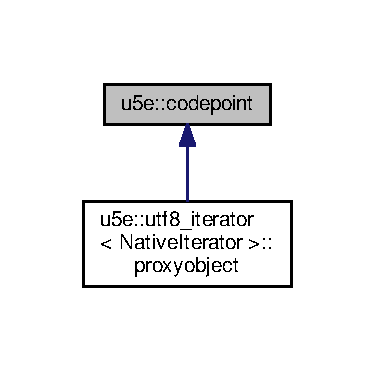
\includegraphics[width=180pt]{classu5e_1_1codepoint__inherit__graph}
\end{center}
\end{figure}
\subsection*{Public Member Functions}
\begin{DoxyCompactItemize}
\item 
constexpr \hyperlink{classu5e_1_1codepoint_a6125584b5079e2ca72f4930e2890ac6d}{codepoint} ()
\item 
constexpr \hyperlink{classu5e_1_1codepoint_a2d033712b1118e34f32e067bf8c90e50}{codepoint} (int32\+\_\+t v)
\item 
constexpr \hyperlink{classu5e_1_1codepoint_a84c5769315b27a56cbf8c077d10c3f79}{codepoint} (const \hyperlink{classu5e_1_1codepoint}{codepoint} \&x)=default
\item 
constexpr \hyperlink{classu5e_1_1codepoint}{codepoint} \& \hyperlink{classu5e_1_1codepoint_a60cccd31a7d78336ffb226df79e2fb58}{operator=} (const \hyperlink{classu5e_1_1codepoint}{codepoint} \&x)=default
\item 
constexpr \hyperlink{classu5e_1_1codepoint}{codepoint} \& \hyperlink{classu5e_1_1codepoint_a06f7e693dc997163c98d9a42fb069b71}{operator=} (int c)
\item 
constexpr \hyperlink{classu5e_1_1codepoint_a62f2f28a2cd7c7f59a13e98deacf3249}{operator int} () const 
\end{DoxyCompactItemize}
\subsection*{Public Attributes}
\begin{DoxyCompactItemize}
\item 
\hyperlink{classu5e_1_1codepoint__traits_a11f00d20915e28671519ef0c96fab05d}{codepoint\+\_\+traits\+::int\+\_\+type} \hyperlink{classu5e_1_1codepoint_ae9340f920cdb4f6615647cbd8dc0fc84}{value}
\end{DoxyCompactItemize}


\subsection{Detailed Description}
Native representation of a codepoint. 

Explicity class in order to hijack overloads, such that we only build codepoints out of known encodings and we only write to encodings out of known codepoints. 

Definition at line 15 of file codepoint.\+hpp.



\subsection{Constructor \& Destructor Documentation}
\index{u5e\+::codepoint@{u5e\+::codepoint}!codepoint@{codepoint}}
\index{codepoint@{codepoint}!u5e\+::codepoint@{u5e\+::codepoint}}
\subsubsection[{\texorpdfstring{codepoint()}{codepoint()}}]{\setlength{\rightskip}{0pt plus 5cm}constexpr u5e\+::codepoint\+::codepoint (
\begin{DoxyParamCaption}
{}
\end{DoxyParamCaption}
)\hspace{0.3cm}{\ttfamily [inline]}}\hypertarget{classu5e_1_1codepoint_a6125584b5079e2ca72f4930e2890ac6d}{}\label{classu5e_1_1codepoint_a6125584b5079e2ca72f4930e2890ac6d}
Default constructor, starts as N\+U\+LL. 

Definition at line 25 of file codepoint.\+hpp.

\index{u5e\+::codepoint@{u5e\+::codepoint}!codepoint@{codepoint}}
\index{codepoint@{codepoint}!u5e\+::codepoint@{u5e\+::codepoint}}
\subsubsection[{\texorpdfstring{codepoint(int32\+\_\+t v)}{codepoint(int32_t v)}}]{\setlength{\rightskip}{0pt plus 5cm}constexpr u5e\+::codepoint\+::codepoint (
\begin{DoxyParamCaption}
\item[{int32\+\_\+t}]{v}
\end{DoxyParamCaption}
)\hspace{0.3cm}{\ttfamily [inline]}}\hypertarget{classu5e_1_1codepoint_a2d033712b1118e34f32e067bf8c90e50}{}\label{classu5e_1_1codepoint_a2d033712b1118e34f32e067bf8c90e50}
Implicit constructor from an integer value. 

Definition at line 30 of file codepoint.\+hpp.

\index{u5e\+::codepoint@{u5e\+::codepoint}!codepoint@{codepoint}}
\index{codepoint@{codepoint}!u5e\+::codepoint@{u5e\+::codepoint}}
\subsubsection[{\texorpdfstring{codepoint(const codepoint \&x)=default}{codepoint(const codepoint &x)=default}}]{\setlength{\rightskip}{0pt plus 5cm}constexpr u5e\+::codepoint\+::codepoint (
\begin{DoxyParamCaption}
\item[{const {\bf codepoint} \&}]{x}
\end{DoxyParamCaption}
)\hspace{0.3cm}{\ttfamily [default]}}\hypertarget{classu5e_1_1codepoint_a84c5769315b27a56cbf8c077d10c3f79}{}\label{classu5e_1_1codepoint_a84c5769315b27a56cbf8c077d10c3f79}
Copy constructor. 

\subsection{Member Function Documentation}
\index{u5e\+::codepoint@{u5e\+::codepoint}!operator int@{operator int}}
\index{operator int@{operator int}!u5e\+::codepoint@{u5e\+::codepoint}}
\subsubsection[{\texorpdfstring{operator int() const }{operator int() const }}]{\setlength{\rightskip}{0pt plus 5cm}constexpr u5e\+::codepoint\+::operator int (
\begin{DoxyParamCaption}
{}
\end{DoxyParamCaption}
) const\hspace{0.3cm}{\ttfamily [inline]}}\hypertarget{classu5e_1_1codepoint_a62f2f28a2cd7c7f59a13e98deacf3249}{}\label{classu5e_1_1codepoint_a62f2f28a2cd7c7f59a13e98deacf3249}
Override int operator to return the codepoint value. 

Definition at line 50 of file codepoint.\+hpp.

\index{u5e\+::codepoint@{u5e\+::codepoint}!operator=@{operator=}}
\index{operator=@{operator=}!u5e\+::codepoint@{u5e\+::codepoint}}
\subsubsection[{\texorpdfstring{operator=(const codepoint \&x)=default}{operator=(const codepoint &x)=default}}]{\setlength{\rightskip}{0pt plus 5cm}constexpr {\bf codepoint}\& u5e\+::codepoint\+::operator= (
\begin{DoxyParamCaption}
\item[{const {\bf codepoint} \&}]{x}
\end{DoxyParamCaption}
)\hspace{0.3cm}{\ttfamily [default]}}\hypertarget{classu5e_1_1codepoint_a60cccd31a7d78336ffb226df79e2fb58}{}\label{classu5e_1_1codepoint_a60cccd31a7d78336ffb226df79e2fb58}
Assignment operator from another codepoint. \index{u5e\+::codepoint@{u5e\+::codepoint}!operator=@{operator=}}
\index{operator=@{operator=}!u5e\+::codepoint@{u5e\+::codepoint}}
\subsubsection[{\texorpdfstring{operator=(int c)}{operator=(int c)}}]{\setlength{\rightskip}{0pt plus 5cm}constexpr {\bf codepoint}\& u5e\+::codepoint\+::operator= (
\begin{DoxyParamCaption}
\item[{int}]{c}
\end{DoxyParamCaption}
)\hspace{0.3cm}{\ttfamily [inline]}}\hypertarget{classu5e_1_1codepoint_a06f7e693dc997163c98d9a42fb069b71}{}\label{classu5e_1_1codepoint_a06f7e693dc997163c98d9a42fb069b71}
Assignment operator from an int. 

Definition at line 45 of file codepoint.\+hpp.



\subsection{Member Data Documentation}
\index{u5e\+::codepoint@{u5e\+::codepoint}!value@{value}}
\index{value@{value}!u5e\+::codepoint@{u5e\+::codepoint}}
\subsubsection[{\texorpdfstring{value}{value}}]{\setlength{\rightskip}{0pt plus 5cm}{\bf codepoint\+\_\+traits\+::int\+\_\+type} u5e\+::codepoint\+::value}\hypertarget{classu5e_1_1codepoint_ae9340f920cdb4f6615647cbd8dc0fc84}{}\label{classu5e_1_1codepoint_ae9340f920cdb4f6615647cbd8dc0fc84}
A codepoint has an integer value type. 

Definition at line 20 of file codepoint.\+hpp.



The documentation for this class was generated from the following file\+:\begin{DoxyCompactItemize}
\item 
u5e/codepoint.\+hpp\end{DoxyCompactItemize}

\hypertarget{classu5e_1_1codepoint__traits}{}\section{u5e\+:\+:codepoint\+\_\+traits Class Reference}
\label{classu5e_1_1codepoint__traits}\index{u5e\+::codepoint\+\_\+traits@{u5e\+::codepoint\+\_\+traits}}


Type information for codepoint.  




{\ttfamily \#include $<$u5e/codepoint\+\_\+traits.\+hpp$>$}

\subsection*{Public Types}
{\bf }\par
\begin{DoxyCompactItemize}
\item 
typedef int32\+\_\+t \hyperlink{classu5e_1_1codepoint__traits_a11f00d20915e28671519ef0c96fab05d}{int\+\_\+type}
\item 
typedef uint32\+\_\+t \hyperlink{classu5e_1_1codepoint__traits_afb5588dd802b42f267a6c254ad7842f1}{pos\+\_\+type}
\item 
typedef int32\+\_\+t \hyperlink{classu5e_1_1codepoint__traits_ab169bad68f239d5248f82749a2962346}{off\+\_\+type}
\end{DoxyCompactItemize}



\subsection{Detailed Description}
Type information for codepoint. 

This class exists only to provide an interface similar to that of the stream and string types. But it is not truly parameterizable, since a codepoint always means the same thing. 

Definition at line 14 of file codepoint\+\_\+traits.\+hpp.



\subsection{Member Typedef Documentation}
\index{u5e\+::codepoint\+\_\+traits@{u5e\+::codepoint\+\_\+traits}!int\+\_\+type@{int\+\_\+type}}
\index{int\+\_\+type@{int\+\_\+type}!u5e\+::codepoint\+\_\+traits@{u5e\+::codepoint\+\_\+traits}}
\subsubsection[{\texorpdfstring{int\+\_\+type}{int_type}}]{\setlength{\rightskip}{0pt plus 5cm}typedef int32\+\_\+t {\bf u5e\+::codepoint\+\_\+traits\+::int\+\_\+type}}\hypertarget{classu5e_1_1codepoint__traits_a11f00d20915e28671519ef0c96fab05d}{}\label{classu5e_1_1codepoint__traits_a11f00d20915e28671519ef0c96fab05d}
Basic meta-\/description of a codepoint 

Definition at line 20 of file codepoint\+\_\+traits.\+hpp.

\index{u5e\+::codepoint\+\_\+traits@{u5e\+::codepoint\+\_\+traits}!off\+\_\+type@{off\+\_\+type}}
\index{off\+\_\+type@{off\+\_\+type}!u5e\+::codepoint\+\_\+traits@{u5e\+::codepoint\+\_\+traits}}
\subsubsection[{\texorpdfstring{off\+\_\+type}{off_type}}]{\setlength{\rightskip}{0pt plus 5cm}typedef int32\+\_\+t {\bf u5e\+::codepoint\+\_\+traits\+::off\+\_\+type}}\hypertarget{classu5e_1_1codepoint__traits_ab169bad68f239d5248f82749a2962346}{}\label{classu5e_1_1codepoint__traits_ab169bad68f239d5248f82749a2962346}
Basic meta-\/description of a codepoint 

Definition at line 22 of file codepoint\+\_\+traits.\+hpp.

\index{u5e\+::codepoint\+\_\+traits@{u5e\+::codepoint\+\_\+traits}!pos\+\_\+type@{pos\+\_\+type}}
\index{pos\+\_\+type@{pos\+\_\+type}!u5e\+::codepoint\+\_\+traits@{u5e\+::codepoint\+\_\+traits}}
\subsubsection[{\texorpdfstring{pos\+\_\+type}{pos_type}}]{\setlength{\rightskip}{0pt plus 5cm}typedef uint32\+\_\+t {\bf u5e\+::codepoint\+\_\+traits\+::pos\+\_\+type}}\hypertarget{classu5e_1_1codepoint__traits_afb5588dd802b42f267a6c254ad7842f1}{}\label{classu5e_1_1codepoint__traits_afb5588dd802b42f267a6c254ad7842f1}
Basic meta-\/description of a codepoint 

Definition at line 21 of file codepoint\+\_\+traits.\+hpp.



The documentation for this class was generated from the following file\+:\begin{DoxyCompactItemize}
\item 
u5e/codepoint\+\_\+traits.\+hpp\end{DoxyCompactItemize}

\hypertarget{classu5e_1_1props_1_1compatibility__and__canonical__decomposition__mapping}{}\section{u5e\+:\+:props\+:\+:compatibility\+\_\+and\+\_\+canonical\+\_\+decomposition\+\_\+mapping Class Reference}
\label{classu5e_1_1props_1_1compatibility__and__canonical__decomposition__mapping}\index{u5e\+::props\+::compatibility\+\_\+and\+\_\+canonical\+\_\+decomposition\+\_\+mapping@{u5e\+::props\+::compatibility\+\_\+and\+\_\+canonical\+\_\+decomposition\+\_\+mapping}}


Subset of Decomposition\+\_\+\+Mapping attribute.  




{\ttfamily \#include $<$u5e/props/compatibility\+\_\+and\+\_\+canonical\+\_\+decomposition\+\_\+mapping.\+hpp$>$}

\subsection*{Static Public Member Functions}
\begin{DoxyCompactItemize}
\item 
static int const $\ast$const \hyperlink{classu5e_1_1props_1_1compatibility__and__canonical__decomposition__mapping_a200596c1d9b890d1bdd02cfaaecdf1de}{resolve} (int input)
\end{DoxyCompactItemize}


\subsection{Detailed Description}
Subset of Decomposition\+\_\+\+Mapping attribute. 

This recursively resolves the canonical decomposition mapping. The returned data is fully compat and canonically decomposed. 

Definition at line 15 of file compatibility\+\_\+and\+\_\+canonical\+\_\+decomposition\+\_\+mapping.\+hpp.



\subsection{Member Function Documentation}
\index{u5e\+::props\+::compatibility\+\_\+and\+\_\+canonical\+\_\+decomposition\+\_\+mapping@{u5e\+::props\+::compatibility\+\_\+and\+\_\+canonical\+\_\+decomposition\+\_\+mapping}!resolve@{resolve}}
\index{resolve@{resolve}!u5e\+::props\+::compatibility\+\_\+and\+\_\+canonical\+\_\+decomposition\+\_\+mapping@{u5e\+::props\+::compatibility\+\_\+and\+\_\+canonical\+\_\+decomposition\+\_\+mapping}}
\subsubsection[{\texorpdfstring{resolve(int input)}{resolve(int input)}}]{\setlength{\rightskip}{0pt plus 5cm}static int const$\ast$ const u5e\+::props\+::compatibility\+\_\+and\+\_\+canonical\+\_\+decomposition\+\_\+mapping\+::resolve (
\begin{DoxyParamCaption}
\item[{int}]{input}
\end{DoxyParamCaption}
)\hspace{0.3cm}{\ttfamily [static]}}\hypertarget{classu5e_1_1props_1_1compatibility__and__canonical__decomposition__mapping_a200596c1d9b890d1bdd02cfaaecdf1de}{}\label{classu5e_1_1props_1_1compatibility__and__canonical__decomposition__mapping_a200596c1d9b890d1bdd02cfaaecdf1de}
Perform the decomposition. Returns N\+U\+LL if the character has no decomposition.

The returned int array will be zero terminated. 

The documentation for this class was generated from the following file\+:\begin{DoxyCompactItemize}
\item 
u5e/props/compatibility\+\_\+and\+\_\+canonical\+\_\+decomposition\+\_\+mapping.\+hpp\end{DoxyCompactItemize}

\hypertarget{classu5e_1_1encoding__assertion}{}\section{u5e\+:\+:encoding\+\_\+assertion$<$ B\+U\+F\+F\+E\+R\+T\+Y\+PE, T $>$ Class Template Reference}
\label{classu5e_1_1encoding__assertion}\index{u5e\+::encoding\+\_\+assertion$<$ B\+U\+F\+F\+E\+R\+T\+Y\+P\+E, T $>$@{u5e\+::encoding\+\_\+assertion$<$ B\+U\+F\+F\+E\+R\+T\+Y\+P\+E, T $>$}}


Assert the encoding matches the native type.  




{\ttfamily \#include $<$u5e/encoding\+\_\+assertion.\+hpp$>$}



\subsection{Detailed Description}
\subsubsection*{template$<$typename B\+U\+F\+F\+E\+R\+T\+Y\+PE, typename T$>$\\*
class u5e\+::encoding\+\_\+assertion$<$ B\+U\+F\+F\+E\+R\+T\+Y\+P\+E, T $>$}

Assert the encoding matches the native type. 

Tests that the encoding can be used with the specific native string type. 

Definition at line 15 of file encoding\+\_\+assertion.\+hpp.



The documentation for this class was generated from the following file\+:\begin{DoxyCompactItemize}
\item 
u5e/encoding\+\_\+assertion.\+hpp\end{DoxyCompactItemize}

\hypertarget{classu5e_1_1props_1_1grapheme__cluster__break}{}\section{u5e\+:\+:props\+:\+:grapheme\+\_\+cluster\+\_\+break Class Reference}
\label{classu5e_1_1props_1_1grapheme__cluster__break}\index{u5e\+::props\+::grapheme\+\_\+cluster\+\_\+break@{u5e\+::props\+::grapheme\+\_\+cluster\+\_\+break}}


Grapheme Cluster Break property for a codepoint.  




{\ttfamily \#include $<$u5e/props/grapheme\+\_\+cluster\+\_\+break.\+hpp$>$}

\subsection*{Public Types}
\begin{DoxyCompactItemize}
\item 
enum \hyperlink{classu5e_1_1props_1_1grapheme__cluster__break_a49537cfb39f9510acd4096379687cf93}{prop\+\_\+value\+\_\+type} \{ \\*
{\bfseries O\+T\+H\+ER}, 
{\bfseries P\+R\+E\+P\+E\+ND}, 
{\bfseries CR}, 
{\bfseries LF}, 
\\*
{\bfseries C\+O\+N\+T\+R\+OL}, 
{\bfseries E\+X\+T\+E\+ND}, 
{\bfseries R\+E\+G\+I\+O\+N\+A\+L\+\_\+\+I\+N\+D\+I\+C\+A\+T\+OR}, 
{\bfseries S\+P\+A\+C\+I\+N\+G\+M\+A\+RK}, 
\\*
{\bfseries L}, 
{\bfseries V}, 
{\bfseries T}, 
{\bfseries LV}, 
\\*
{\bfseries L\+VT}, 
{\bfseries E\+\_\+\+B\+A\+SE}, 
{\bfseries E\+\_\+\+M\+O\+D\+I\+F\+I\+ER}, 
{\bfseries Z\+WJ}, 
\\*
{\bfseries G\+L\+U\+E\+\_\+\+A\+F\+T\+E\+R\+\_\+\+Z\+WJ}, 
{\bfseries E\+\_\+\+B\+A\+S\+E\+\_\+\+G\+AZ}
 \}
\end{DoxyCompactItemize}
\subsection*{Static Public Member Functions}
\begin{DoxyCompactItemize}
\item 
static \hyperlink{classu5e_1_1props_1_1grapheme__cluster__break_a49537cfb39f9510acd4096379687cf93}{prop\+\_\+value\+\_\+type} \hyperlink{classu5e_1_1props_1_1grapheme__cluster__break_a420baa4462ddbfa46c26a6205c79cd7b}{resolve} (\hyperlink{classu5e_1_1codepoint}{codepoint} c)
\end{DoxyCompactItemize}


\subsection{Detailed Description}
Grapheme Cluster Break property for a codepoint. 

Definition at line 15 of file grapheme\+\_\+cluster\+\_\+break.\+hpp.



\subsection{Member Enumeration Documentation}
\index{u5e\+::props\+::grapheme\+\_\+cluster\+\_\+break@{u5e\+::props\+::grapheme\+\_\+cluster\+\_\+break}!prop\+\_\+value\+\_\+type@{prop\+\_\+value\+\_\+type}}
\index{prop\+\_\+value\+\_\+type@{prop\+\_\+value\+\_\+type}!u5e\+::props\+::grapheme\+\_\+cluster\+\_\+break@{u5e\+::props\+::grapheme\+\_\+cluster\+\_\+break}}
\subsubsection[{\texorpdfstring{prop\+\_\+value\+\_\+type}{prop_value_type}}]{\setlength{\rightskip}{0pt plus 5cm}enum {\bf u5e\+::props\+::grapheme\+\_\+cluster\+\_\+break\+::prop\+\_\+value\+\_\+type}}\hypertarget{classu5e_1_1props_1_1grapheme__cluster__break_a49537cfb39f9510acd4096379687cf93}{}\label{classu5e_1_1props_1_1grapheme__cluster__break_a49537cfb39f9510acd4096379687cf93}
Possible values for the property as specified by the standard 

Definition at line 20 of file grapheme\+\_\+cluster\+\_\+break.\+hpp.



\subsection{Member Function Documentation}
\index{u5e\+::props\+::grapheme\+\_\+cluster\+\_\+break@{u5e\+::props\+::grapheme\+\_\+cluster\+\_\+break}!resolve@{resolve}}
\index{resolve@{resolve}!u5e\+::props\+::grapheme\+\_\+cluster\+\_\+break@{u5e\+::props\+::grapheme\+\_\+cluster\+\_\+break}}
\subsubsection[{\texorpdfstring{resolve(codepoint c)}{resolve(codepoint c)}}]{\setlength{\rightskip}{0pt plus 5cm}static {\bf prop\+\_\+value\+\_\+type} u5e\+::props\+::grapheme\+\_\+cluster\+\_\+break\+::resolve (
\begin{DoxyParamCaption}
\item[{{\bf codepoint}}]{c}
\end{DoxyParamCaption}
)\hspace{0.3cm}{\ttfamily [static]}}\hypertarget{classu5e_1_1props_1_1grapheme__cluster__break_a420baa4462ddbfa46c26a6205c79cd7b}{}\label{classu5e_1_1props_1_1grapheme__cluster__break_a420baa4462ddbfa46c26a6205c79cd7b}
Return the value of the property for the given codepoint by looking at the database. 

The documentation for this class was generated from the following file\+:\begin{DoxyCompactItemize}
\item 
u5e/props/grapheme\+\_\+cluster\+\_\+break.\+hpp\end{DoxyCompactItemize}

\hypertarget{classu5e_1_1iterator__assertion}{}\section{u5e\+:\+:iterator\+\_\+assertion$<$ W\+R\+A\+P\+P\+ED, T $>$ Class Template Reference}
\label{classu5e_1_1iterator__assertion}\index{u5e\+::iterator\+\_\+assertion$<$ W\+R\+A\+P\+P\+E\+D, T $>$@{u5e\+::iterator\+\_\+assertion$<$ W\+R\+A\+P\+P\+E\+D, T $>$}}


Asserts the iterator is consistently defined.  




{\ttfamily \#include $<$u5e/iterator\+\_\+assertion.\+hpp$>$}



Inheritance diagram for u5e\+:\+:iterator\+\_\+assertion$<$ W\+R\+A\+P\+P\+ED, T $>$\+:
\nopagebreak
\begin{figure}[H]
\begin{center}
\leavevmode
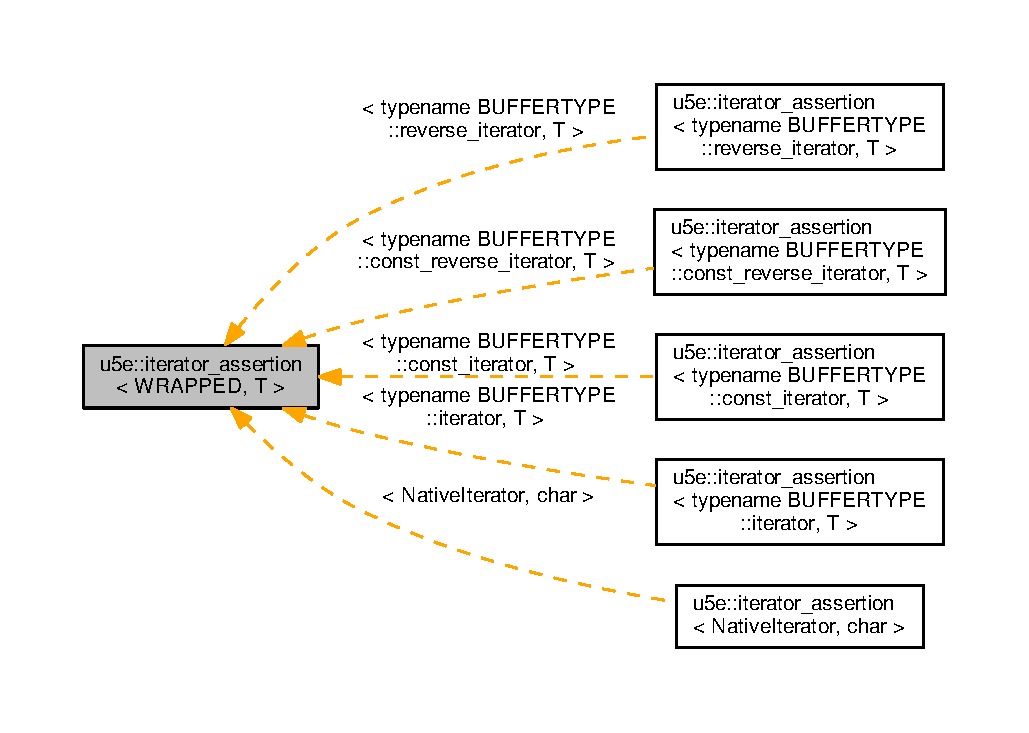
\includegraphics[width=350pt]{classu5e_1_1iterator__assertion__inherit__graph}
\end{center}
\end{figure}


\subsection{Detailed Description}
\subsubsection*{template$<$typename W\+R\+A\+P\+P\+ED, typename T$>$\\*
class u5e\+::iterator\+\_\+assertion$<$ W\+R\+A\+P\+P\+E\+D, T $>$}

Asserts the iterator is consistently defined. 

Definition at line 11 of file iterator\+\_\+assertion.\+hpp.



The documentation for this class was generated from the following file\+:\begin{DoxyCompactItemize}
\item 
u5e/iterator\+\_\+assertion.\+hpp\end{DoxyCompactItemize}

\hypertarget{classu5e_1_1utf8__iterator_1_1proxyobject}{}\section{u5e\+:\+:utf8\+\_\+iterator$<$ Native\+Iterator $>$\+:\+:proxyobject Class Reference}
\label{classu5e_1_1utf8__iterator_1_1proxyobject}\index{u5e\+::utf8\+\_\+iterator$<$ Native\+Iterator $>$\+::proxyobject@{u5e\+::utf8\+\_\+iterator$<$ Native\+Iterator $>$\+::proxyobject}}


offers write access to the iterator at a given position  




{\ttfamily \#include $<$u5e/utf8\+\_\+iterator.\+hpp$>$}



Inheritance diagram for u5e\+:\+:utf8\+\_\+iterator$<$ Native\+Iterator $>$\+:\+:proxyobject\+:
\nopagebreak
\begin{figure}[H]
\begin{center}
\leavevmode
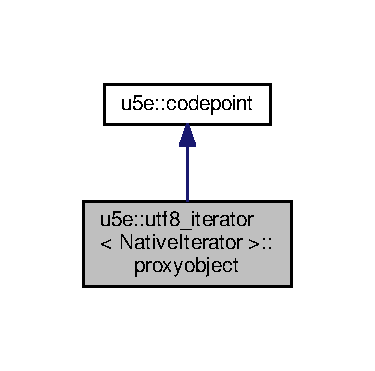
\includegraphics[width=180pt]{classu5e_1_1utf8__iterator_1_1proxyobject__inherit__graph}
\end{center}
\end{figure}


Collaboration diagram for u5e\+:\+:utf8\+\_\+iterator$<$ Native\+Iterator $>$\+:\+:proxyobject\+:
\nopagebreak
\begin{figure}[H]
\begin{center}
\leavevmode
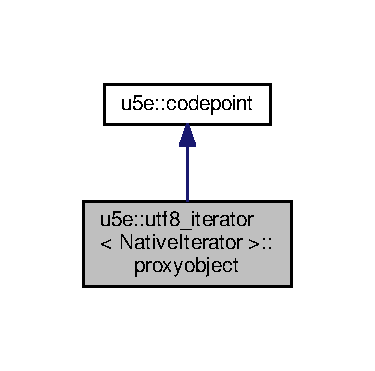
\includegraphics[width=180pt]{classu5e_1_1utf8__iterator_1_1proxyobject__coll__graph}
\end{center}
\end{figure}
\subsection*{Public Member Functions}
\begin{DoxyCompactItemize}
\item 
\hyperlink{classu5e_1_1utf8__iterator_1_1proxyobject_a81e1a4e72b44fb59be44669304dcf741}{proxyobject} (\hyperlink{classu5e_1_1utf8__iterator}{utf8\+\_\+iterator}$<$ Native\+Iterator $>$ \&refin)
\item 
\hyperlink{classu5e_1_1utf8__iterator_1_1proxyobject}{proxyobject} \& \hyperlink{classu5e_1_1utf8__iterator_1_1proxyobject_a7e78eebdd29c280b3b39da10a259a8f3}{operator=} (const \hyperlink{classu5e_1_1codepoint}{codepoint} c)
\end{DoxyCompactItemize}
\subsection*{Additional Inherited Members}


\subsection{Detailed Description}
\subsubsection*{template$<$typename Native\+Iterator$>$\\*
class u5e\+::utf8\+\_\+iterator$<$ Native\+Iterator $>$\+::proxyobject}

offers write access to the iterator at a given position 

This is necessary because operator= can only be done after operator$\ast$ is executed, this wouldn\textquotesingle{}t be necessary if there was a dedicated operator for \textquotesingle{}assign to the dereference\textquotesingle{}. 

Definition at line 292 of file utf8\+\_\+iterator.\+hpp.



\subsection{Constructor \& Destructor Documentation}
\index{u5e\+::utf8\+\_\+iterator\+::proxyobject@{u5e\+::utf8\+\_\+iterator\+::proxyobject}!proxyobject@{proxyobject}}
\index{proxyobject@{proxyobject}!u5e\+::utf8\+\_\+iterator\+::proxyobject@{u5e\+::utf8\+\_\+iterator\+::proxyobject}}
\subsubsection[{\texorpdfstring{proxyobject(utf8\+\_\+iterator$<$ Native\+Iterator $>$ \&refin)}{proxyobject(utf8_iterator< NativeIterator > &refin)}}]{\setlength{\rightskip}{0pt plus 5cm}template$<$typename Native\+Iterator$>$ {\bf u5e\+::utf8\+\_\+iterator}$<$ Native\+Iterator $>$\+::proxyobject\+::proxyobject (
\begin{DoxyParamCaption}
\item[{{\bf utf8\+\_\+iterator}$<$ Native\+Iterator $>$ \&}]{refin}
\end{DoxyParamCaption}
)\hspace{0.3cm}{\ttfamily [inline]}}\hypertarget{classu5e_1_1utf8__iterator_1_1proxyobject_a81e1a4e72b44fb59be44669304dcf741}{}\label{classu5e_1_1utf8__iterator_1_1proxyobject_a81e1a4e72b44fb59be44669304dcf741}
Create from the iterator 

Definition at line 303 of file utf8\+\_\+iterator.\+hpp.



\subsection{Member Function Documentation}
\index{u5e\+::utf8\+\_\+iterator\+::proxyobject@{u5e\+::utf8\+\_\+iterator\+::proxyobject}!operator=@{operator=}}
\index{operator=@{operator=}!u5e\+::utf8\+\_\+iterator\+::proxyobject@{u5e\+::utf8\+\_\+iterator\+::proxyobject}}
\subsubsection[{\texorpdfstring{operator=(const codepoint c)}{operator=(const codepoint c)}}]{\setlength{\rightskip}{0pt plus 5cm}template$<$typename Native\+Iterator$>$ {\bf proxyobject}\& {\bf u5e\+::utf8\+\_\+iterator}$<$ Native\+Iterator $>$\+::proxyobject\+::operator= (
\begin{DoxyParamCaption}
\item[{const {\bf codepoint}}]{c}
\end{DoxyParamCaption}
)\hspace{0.3cm}{\ttfamily [inline]}}\hypertarget{classu5e_1_1utf8__iterator_1_1proxyobject_a7e78eebdd29c280b3b39da10a259a8f3}{}\label{classu5e_1_1utf8__iterator_1_1proxyobject_a7e78eebdd29c280b3b39da10a259a8f3}
Assign a codepoint to this position, writing as many octets as necessary. Note that if you do this in the middle of a string, there is a likely chance that you will render the remainder of the string invalid. So it\textquotesingle{}s really only a good idea to do this as an \char`\"{}append\char`\"{} operation. 

Definition at line 316 of file utf8\+\_\+iterator.\+hpp.



The documentation for this class was generated from the following file\+:\begin{DoxyCompactItemize}
\item 
u5e/utf8\+\_\+iterator.\+hpp\end{DoxyCompactItemize}

\hypertarget{classu5e_1_1version_1_1run__time}{}\section{u5e\+:\+:version\+:\+:run\+\_\+time Class Reference}
\label{classu5e_1_1version_1_1run__time}\index{u5e\+::version\+::run\+\_\+time@{u5e\+::version\+::run\+\_\+time}}


introspection for run-\/time version declaration To test which version of the library are you linking against  




{\ttfamily \#include $<$u5e/version.\+hpp$>$}

\subsection*{Static Public Attributes}
{\bf }\par
\begin{DoxyCompactItemize}
\item 
static const int \hyperlink{classu5e_1_1version_1_1run__time_af9ae22e12e9f02e28d5e6969a038f1f5}{major}\hypertarget{classu5e_1_1version_1_1run__time_af9ae22e12e9f02e28d5e6969a038f1f5}{}\label{classu5e_1_1version_1_1run__time_af9ae22e12e9f02e28d5e6969a038f1f5}

\begin{DoxyCompactList}\small\item\em Run-\/time introspection for library version. \end{DoxyCompactList}\item 
static const int \hyperlink{classu5e_1_1version_1_1run__time_a2a7f0813841d742afe86ad0899fbd046}{minor}\hypertarget{classu5e_1_1version_1_1run__time_a2a7f0813841d742afe86ad0899fbd046}{}\label{classu5e_1_1version_1_1run__time_a2a7f0813841d742afe86ad0899fbd046}

\begin{DoxyCompactList}\small\item\em Run-\/time introspection for library version. \end{DoxyCompactList}\item 
static const int \hyperlink{classu5e_1_1version_1_1run__time_ab97c8f0bff8d8dbdf901693135f2411f}{patch}\hypertarget{classu5e_1_1version_1_1run__time_ab97c8f0bff8d8dbdf901693135f2411f}{}\label{classu5e_1_1version_1_1run__time_ab97c8f0bff8d8dbdf901693135f2411f}

\begin{DoxyCompactList}\small\item\em Run-\/time introspection for library version. \end{DoxyCompactList}\end{DoxyCompactItemize}



\subsection{Detailed Description}
introspection for run-\/time version declaration To test which version of the library are you linking against 

Definition at line 30 of file version.\+hpp.



The documentation for this class was generated from the following file\+:\begin{DoxyCompactItemize}
\item 
u5e/version.\+hpp\end{DoxyCompactItemize}

\hypertarget{classu5e_1_1utf32ne}{}\section{u5e\+:\+:utf32ne Class Reference}
\label{classu5e_1_1utf32ne}\index{u5e\+::utf32ne@{u5e\+::utf32ne}}


Architecture-\/specific type to interface U\+T\+F32\+BE or U\+T\+F32\+LE.  




{\ttfamily \#include $<$u5e/utf32ne.\+hpp$>$}

\begin{DoxyCompactItemize}
\item 
{\footnotesize template$<$typename Native\+String $>$ }\\using \hyperlink{classu5e_1_1utf32ne_aa94f3484382747653c46ce429612eedc}{iterator} = typename Native\+String\+::iterator
\item 
{\footnotesize template$<$typename Native\+String $>$ }\\using \hyperlink{classu5e_1_1utf32ne_a4d281b04b01e996702b02445fa25fc76}{const\+\_\+iterator} = typename Native\+String\+::const\+\_\+iterator
\item 
{\footnotesize template$<$typename Native\+String $>$ }\\static Native\+String\+::const\+\_\+iterator \hyperlink{classu5e_1_1utf32ne_a9ab16ff63de47e7f02532d03af7b70c1}{native\+\_\+const\+\_\+iterator} (typename Native\+String\+::const\+\_\+iterator it)
\item 
{\footnotesize template$<$typename Input\+Native\+Iterator , typename Output\+Native\+String $>$ }\\static void \hyperlink{classu5e_1_1utf32ne_a6678bc31c37d8b740ea3fd47d572774b}{append\+\_\+from\+\_\+utf32ne} (Input\+Native\+Iterator first, Input\+Native\+Iterator last, Output\+Native\+String \&output)
\end{DoxyCompactItemize}


\subsection{Detailed Description}
Architecture-\/specific type to interface U\+T\+F32\+BE or U\+T\+F32\+LE. 

\hyperlink{classu5e_1_1utf32ne}{utf32ne} is not an encoding. It is a type that should be used to interface with either U\+T\+F32\+BE or with U\+T\+F32\+LE depending on what the native endianess is.

Because utf32 with the native endianess can be used natively, there\textquotesingle{}s no special logic and everything is delegated to the native types. 

Definition at line 20 of file utf32ne.\+hpp.



\subsection{Member Typedef Documentation}
\index{u5e\+::utf32ne@{u5e\+::utf32ne}!const\+\_\+iterator@{const\+\_\+iterator}}
\index{const\+\_\+iterator@{const\+\_\+iterator}!u5e\+::utf32ne@{u5e\+::utf32ne}}
\subsubsection[{\texorpdfstring{const\+\_\+iterator}{const_iterator}}]{\setlength{\rightskip}{0pt plus 5cm}template$<$typename Native\+String $>$ using {\bf u5e\+::utf32ne\+::const\+\_\+iterator} =  typename Native\+String\+::const\+\_\+iterator}\hypertarget{classu5e_1_1utf32ne_a4d281b04b01e996702b02445fa25fc76}{}\label{classu5e_1_1utf32ne_a4d281b04b01e996702b02445fa25fc76}
Delegate to the underlying iterator 

Definition at line 30 of file utf32ne.\+hpp.

\index{u5e\+::utf32ne@{u5e\+::utf32ne}!iterator@{iterator}}
\index{iterator@{iterator}!u5e\+::utf32ne@{u5e\+::utf32ne}}
\subsubsection[{\texorpdfstring{iterator}{iterator}}]{\setlength{\rightskip}{0pt plus 5cm}template$<$typename Native\+String $>$ using {\bf u5e\+::utf32ne\+::iterator} =  typename Native\+String\+::iterator}\hypertarget{classu5e_1_1utf32ne_aa94f3484382747653c46ce429612eedc}{}\label{classu5e_1_1utf32ne_aa94f3484382747653c46ce429612eedc}
Delegate to the underlying iterator 

Definition at line 27 of file utf32ne.\+hpp.



\subsection{Member Function Documentation}
\index{u5e\+::utf32ne@{u5e\+::utf32ne}!append\+\_\+from\+\_\+utf32ne@{append\+\_\+from\+\_\+utf32ne}}
\index{append\+\_\+from\+\_\+utf32ne@{append\+\_\+from\+\_\+utf32ne}!u5e\+::utf32ne@{u5e\+::utf32ne}}
\subsubsection[{\texorpdfstring{append\+\_\+from\+\_\+utf32ne(\+Input\+Native\+Iterator first, Input\+Native\+Iterator last, Output\+Native\+String \&output)}{append_from_utf32ne(InputNativeIterator first, InputNativeIterator last, OutputNativeString &output)}}]{\setlength{\rightskip}{0pt plus 5cm}template$<$typename Input\+Native\+Iterator , typename Output\+Native\+String $>$ static void u5e\+::utf32ne\+::append\+\_\+from\+\_\+utf32ne (
\begin{DoxyParamCaption}
\item[{Input\+Native\+Iterator}]{first, }
\item[{Input\+Native\+Iterator}]{last, }
\item[{Output\+Native\+String \&}]{output}
\end{DoxyParamCaption}
)\hspace{0.3cm}{\ttfamily [inline]}, {\ttfamily [static]}}\hypertarget{classu5e_1_1utf32ne_a6678bc31c37d8b740ea3fd47d572774b}{}\label{classu5e_1_1utf32ne_a6678bc31c37d8b740ea3fd47d572774b}
Delegate to the underlying iterator 

Definition at line 40 of file utf32ne.\+hpp.

\index{u5e\+::utf32ne@{u5e\+::utf32ne}!native\+\_\+const\+\_\+iterator@{native\+\_\+const\+\_\+iterator}}
\index{native\+\_\+const\+\_\+iterator@{native\+\_\+const\+\_\+iterator}!u5e\+::utf32ne@{u5e\+::utf32ne}}
\subsubsection[{\texorpdfstring{native\+\_\+const\+\_\+iterator(typename Native\+String\+::const\+\_\+iterator it)}{native_const_iterator(typename NativeString::const_iterator it)}}]{\setlength{\rightskip}{0pt plus 5cm}template$<$typename Native\+String $>$ static Native\+String\+::const\+\_\+iterator u5e\+::utf32ne\+::native\+\_\+const\+\_\+iterator (
\begin{DoxyParamCaption}
\item[{typename Native\+String\+::const\+\_\+iterator}]{it}
\end{DoxyParamCaption}
)\hspace{0.3cm}{\ttfamily [inline]}, {\ttfamily [static]}}\hypertarget{classu5e_1_1utf32ne_a9ab16ff63de47e7f02532d03af7b70c1}{}\label{classu5e_1_1utf32ne_a9ab16ff63de47e7f02532d03af7b70c1}
Delegate to the underlying iterator 

Definition at line 34 of file utf32ne.\+hpp.



The documentation for this class was generated from the following file\+:\begin{DoxyCompactItemize}
\item 
u5e/utf32ne.\+hpp\end{DoxyCompactItemize}

\hypertarget{classu5e_1_1utf32ne__string}{}\section{u5e\+:\+:utf32ne\+\_\+string Class Reference}
\label{classu5e_1_1utf32ne__string}\index{u5e\+::utf32ne\+\_\+string@{u5e\+::utf32ne\+\_\+string}}


Typedef\+: \hyperlink{classu5e_1_1basic__encodedstring}{basic\+\_\+encodedstring} of \hyperlink{classu5e_1_1utf32ne}{utf32ne} and std\+::basic\+\_\+string$<$int$>$  




{\ttfamily \#include $<$u5e/utf32ne\+\_\+string.\+hpp$>$}



\subsection{Detailed Description}
Typedef\+: \hyperlink{classu5e_1_1basic__encodedstring}{basic\+\_\+encodedstring} of \hyperlink{classu5e_1_1utf32ne}{utf32ne} and std\+::basic\+\_\+string$<$int$>$ 

Although this is a typedef, it shows up in doxygen as a class for better discoverability. 

The documentation for this class was generated from the following file\+:\begin{DoxyCompactItemize}
\item 
u5e/utf32ne\+\_\+string.\+hpp\end{DoxyCompactItemize}

\hypertarget{classu5e_1_1utf32ne__string__grapheme}{}\section{u5e\+:\+:utf32ne\+\_\+string\+\_\+grapheme Class Reference}
\label{classu5e_1_1utf32ne__string__grapheme}\index{u5e\+::utf32ne\+\_\+string\+\_\+grapheme@{u5e\+::utf32ne\+\_\+string\+\_\+grapheme}}


Typedef\+: \hyperlink{classu5e_1_1basic__grapheme}{basic\+\_\+grapheme} of \hyperlink{classu5e_1_1utf32ne__string}{utf32ne\+\_\+string}.  




{\ttfamily \#include $<$u5e/utf32ne\+\_\+string\+\_\+grapheme.\+hpp$>$}



\subsection{Detailed Description}
Typedef\+: \hyperlink{classu5e_1_1basic__grapheme}{basic\+\_\+grapheme} of \hyperlink{classu5e_1_1utf32ne__string}{utf32ne\+\_\+string}. 

Although this is a typedef, it shows up in doxygen as a class for better discoverability. 

The documentation for this class was generated from the following file\+:\begin{DoxyCompactItemize}
\item 
u5e/utf32ne\+\_\+string\+\_\+grapheme.\+hpp\end{DoxyCompactItemize}

\hypertarget{classu5e_1_1utf32ne__string__grapheme__iterator}{}\section{u5e\+:\+:utf32ne\+\_\+string\+\_\+grapheme\+\_\+iterator Class Reference}
\label{classu5e_1_1utf32ne__string__grapheme__iterator}\index{u5e\+::utf32ne\+\_\+string\+\_\+grapheme\+\_\+iterator@{u5e\+::utf32ne\+\_\+string\+\_\+grapheme\+\_\+iterator}}


Typedef\+: \hyperlink{classu5e_1_1basic__grapheme__iterator}{basic\+\_\+grapheme\+\_\+iterator} of \hyperlink{classu5e_1_1utf32ne__string}{utf32ne\+\_\+string}.  




{\ttfamily \#include $<$u5e/utf32ne\+\_\+string\+\_\+grapheme\+\_\+iterator.\+hpp$>$}



\subsection{Detailed Description}
Typedef\+: \hyperlink{classu5e_1_1basic__grapheme__iterator}{basic\+\_\+grapheme\+\_\+iterator} of \hyperlink{classu5e_1_1utf32ne__string}{utf32ne\+\_\+string}. 

Although this is a typedef, it shows up in doxygen as a class for better discoverability. 

The documentation for this class was generated from the following file\+:\begin{DoxyCompactItemize}
\item 
u5e/utf32ne\+\_\+string\+\_\+grapheme\+\_\+iterator.\+hpp\end{DoxyCompactItemize}

\hypertarget{classu5e_1_1utf32ne__string__view}{}\section{u5e\+:\+:utf32ne\+\_\+string\+\_\+view Class Reference}
\label{classu5e_1_1utf32ne__string__view}\index{u5e\+::utf32ne\+\_\+string\+\_\+view@{u5e\+::utf32ne\+\_\+string\+\_\+view}}


Typedef\+: \hyperlink{classu5e_1_1basic__encodedstring}{basic\+\_\+encodedstring} of \hyperlink{classu5e_1_1utf32ne}{utf32ne} and basic\+\_\+string\+\_\+view$<$int$>$  




{\ttfamily \#include $<$u5e/utf32ne\+\_\+string\+\_\+view.\+hpp$>$}



\subsection{Detailed Description}
Typedef\+: \hyperlink{classu5e_1_1basic__encodedstring}{basic\+\_\+encodedstring} of \hyperlink{classu5e_1_1utf32ne}{utf32ne} and basic\+\_\+string\+\_\+view$<$int$>$ 

Although this is a typedef, it shows up in doxygen as a class for better discoverability. 

The documentation for this class was generated from the following file\+:\begin{DoxyCompactItemize}
\item 
u5e/utf32ne\+\_\+string\+\_\+view.\+hpp\end{DoxyCompactItemize}

\hypertarget{classu5e_1_1utf32ne__string__view__grapheme}{}\section{u5e\+:\+:utf32ne\+\_\+string\+\_\+view\+\_\+grapheme Class Reference}
\label{classu5e_1_1utf32ne__string__view__grapheme}\index{u5e\+::utf32ne\+\_\+string\+\_\+view\+\_\+grapheme@{u5e\+::utf32ne\+\_\+string\+\_\+view\+\_\+grapheme}}


Typedef\+: \hyperlink{classu5e_1_1basic__grapheme}{basic\+\_\+grapheme} of \hyperlink{classu5e_1_1utf32ne__string__view}{utf32ne\+\_\+string\+\_\+view}.  




{\ttfamily \#include $<$u5e/utf32ne\+\_\+string\+\_\+view\+\_\+grapheme.\+hpp$>$}



\subsection{Detailed Description}
Typedef\+: \hyperlink{classu5e_1_1basic__grapheme}{basic\+\_\+grapheme} of \hyperlink{classu5e_1_1utf32ne__string__view}{utf32ne\+\_\+string\+\_\+view}. 

Although this is a typedef, it shows up in doxygen as a class for better discoverability. 

The documentation for this class was generated from the following file\+:\begin{DoxyCompactItemize}
\item 
u5e/utf32ne\+\_\+string\+\_\+view\+\_\+grapheme.\+hpp\end{DoxyCompactItemize}

\hypertarget{classu5e_1_1utf32ne__string__view__grapheme__iterator}{}\section{u5e\+:\+:utf32ne\+\_\+string\+\_\+view\+\_\+grapheme\+\_\+iterator Class Reference}
\label{classu5e_1_1utf32ne__string__view__grapheme__iterator}\index{u5e\+::utf32ne\+\_\+string\+\_\+view\+\_\+grapheme\+\_\+iterator@{u5e\+::utf32ne\+\_\+string\+\_\+view\+\_\+grapheme\+\_\+iterator}}


Typedef\+: \hyperlink{classu5e_1_1basic__grapheme__iterator}{basic\+\_\+grapheme\+\_\+iterator} of \hyperlink{classu5e_1_1utf32ne__string__view}{utf32ne\+\_\+string\+\_\+view}.  




{\ttfamily \#include $<$u5e/utf32ne\+\_\+string\+\_\+view\+\_\+grapheme\+\_\+iterator.\+hpp$>$}



\subsection{Detailed Description}
Typedef\+: \hyperlink{classu5e_1_1basic__grapheme__iterator}{basic\+\_\+grapheme\+\_\+iterator} of \hyperlink{classu5e_1_1utf32ne__string__view}{utf32ne\+\_\+string\+\_\+view}. 

Although this is a typedef, it shows up in doxygen as a class for better discoverability. 

The documentation for this class was generated from the following file\+:\begin{DoxyCompactItemize}
\item 
u5e/utf32ne\+\_\+string\+\_\+view\+\_\+grapheme\+\_\+iterator.\+hpp\end{DoxyCompactItemize}

\hypertarget{classu5e_1_1utf8}{}\section{u5e\+:\+:utf8 Class Reference}
\label{classu5e_1_1utf8}\index{u5e\+::utf8@{u5e\+::utf8}}


Encoding type for U\+T\+F8 text. Unlike U\+T\+F16 and U\+T\+F32, U\+T\+F8 is endian independent.  




{\ttfamily \#include $<$u5e/utf8.\+hpp$>$}

\subsection*{Public Types}
\begin{DoxyCompactItemize}
\item 
{\footnotesize template$<$typename Native\+String $>$ }\\using \hyperlink{classu5e_1_1utf8_a4a1112036dbaf999d2c7752ac7536ea0}{iterator} = \hyperlink{classu5e_1_1utf8__iterator}{utf8\+\_\+iterator}$<$ typename Native\+String\+::iterator $>$
\item 
{\footnotesize template$<$typename Native\+String $>$ }\\using \hyperlink{classu5e_1_1utf8_a0a0e49f87a51183640beb235c89fd996}{const\+\_\+iterator} = \hyperlink{classu5e_1_1utf8__const__iterator}{utf8\+\_\+const\+\_\+iterator}$<$ typename Native\+String\+::const\+\_\+iterator $>$
\end{DoxyCompactItemize}
\subsection*{Static Public Member Functions}
\begin{DoxyCompactItemize}
\item 
{\footnotesize template$<$typename Native\+String $>$ }\\static Native\+String\+::const\+\_\+iterator \hyperlink{classu5e_1_1utf8_a96aee1a73b68ed1396bf12b469093942}{native\+\_\+const\+\_\+iterator} (\hyperlink{classu5e_1_1utf8__const__iterator}{utf8\+\_\+const\+\_\+iterator}$<$ typename Native\+String\+::const\+\_\+iterator $>$ it)
\item 
{\footnotesize template$<$typename Input\+Native\+Iterator , typename Output\+Native\+String $>$ }\\static void {\bfseries append\+\_\+from\+\_\+utf32ne} (Input\+Native\+Iterator first, Input\+Native\+Iterator last, Output\+Native\+String \&output)\hypertarget{classu5e_1_1utf8_a3b756c2ac9c47477f2cbe89311d559a9}{}\label{classu5e_1_1utf8_a3b756c2ac9c47477f2cbe89311d559a9}

\end{DoxyCompactItemize}


\subsection{Detailed Description}
Encoding type for U\+T\+F8 text. Unlike U\+T\+F16 and U\+T\+F32, U\+T\+F8 is endian independent. 

Definition at line 17 of file utf8.\+hpp.



\subsection{Member Typedef Documentation}
\index{u5e\+::utf8@{u5e\+::utf8}!const\+\_\+iterator@{const\+\_\+iterator}}
\index{const\+\_\+iterator@{const\+\_\+iterator}!u5e\+::utf8@{u5e\+::utf8}}
\subsubsection[{\texorpdfstring{const\+\_\+iterator}{const_iterator}}]{\setlength{\rightskip}{0pt plus 5cm}template$<$typename Native\+String $>$ using {\bf u5e\+::utf8\+::const\+\_\+iterator} =  {\bf utf8\+\_\+const\+\_\+iterator}$<$typename Native\+String\+::const\+\_\+iterator$>$}\hypertarget{classu5e_1_1utf8_a0a0e49f87a51183640beb235c89fd996}{}\label{classu5e_1_1utf8_a0a0e49f87a51183640beb235c89fd996}
Delegated to \hyperlink{classu5e_1_1utf8__const__iterator}{utf8\+\_\+const\+\_\+iterator} of the native type 
\begin{DoxyTemplParams}{Template Parameters}
{\em Native\+String} & the native string type with \hyperlink{classu5e_1_1utf8}{utf8} data \\
\hline
\end{DoxyTemplParams}


Definition at line 34 of file utf8.\+hpp.

\index{u5e\+::utf8@{u5e\+::utf8}!iterator@{iterator}}
\index{iterator@{iterator}!u5e\+::utf8@{u5e\+::utf8}}
\subsubsection[{\texorpdfstring{iterator}{iterator}}]{\setlength{\rightskip}{0pt plus 5cm}template$<$typename Native\+String $>$ using {\bf u5e\+::utf8\+::iterator} =  {\bf utf8\+\_\+iterator}$<$typename Native\+String\+::iterator$>$}\hypertarget{classu5e_1_1utf8_a4a1112036dbaf999d2c7752ac7536ea0}{}\label{classu5e_1_1utf8_a4a1112036dbaf999d2c7752ac7536ea0}
Delegated to \hyperlink{classu5e_1_1utf8__iterator}{utf8\+\_\+iterator} of the native type. 
\begin{DoxyTemplParams}{Template Parameters}
{\em Native\+String} & the native string type with \hyperlink{classu5e_1_1utf8}{utf8} data \\
\hline
\end{DoxyTemplParams}


Definition at line 26 of file utf8.\+hpp.



\subsection{Member Function Documentation}
\index{u5e\+::utf8@{u5e\+::utf8}!native\+\_\+const\+\_\+iterator@{native\+\_\+const\+\_\+iterator}}
\index{native\+\_\+const\+\_\+iterator@{native\+\_\+const\+\_\+iterator}!u5e\+::utf8@{u5e\+::utf8}}
\subsubsection[{\texorpdfstring{native\+\_\+const\+\_\+iterator(utf8\+\_\+const\+\_\+iterator$<$ typename Native\+String\+::const\+\_\+iterator $>$ it)}{native_const_iterator(utf8_const_iterator< typename NativeString::const_iterator > it)}}]{\setlength{\rightskip}{0pt plus 5cm}template$<$typename Native\+String $>$ static Native\+String\+::const\+\_\+iterator u5e\+::utf8\+::native\+\_\+const\+\_\+iterator (
\begin{DoxyParamCaption}
\item[{{\bf utf8\+\_\+const\+\_\+iterator}$<$ typename Native\+String\+::const\+\_\+iterator $>$}]{it}
\end{DoxyParamCaption}
)\hspace{0.3cm}{\ttfamily [inline]}, {\ttfamily [static]}}\hypertarget{classu5e_1_1utf8_a96aee1a73b68ed1396bf12b469093942}{}\label{classu5e_1_1utf8_a96aee1a73b68ed1396bf12b469093942}
Get access to the native const\+\_\+iterator with the native data. 

Definition at line 42 of file utf8.\+hpp.



The documentation for this class was generated from the following file\+:\begin{DoxyCompactItemize}
\item 
u5e/utf8.\+hpp\end{DoxyCompactItemize}

\hypertarget{classu5e_1_1utf8__bounds}{}\section{u5e\+:\+:utf8\+\_\+bounds$<$ Native\+Iterator $>$ Class Template Reference}
\label{classu5e_1_1utf8__bounds}\index{u5e\+::utf8\+\_\+bounds$<$ Native\+Iterator $>$@{u5e\+::utf8\+\_\+bounds$<$ Native\+Iterator $>$}}


Check and enforce bounds of \hyperlink{classu5e_1_1utf8}{utf8} text.  




{\ttfamily \#include $<$u5e/utf8\+\_\+bounds.\+hpp$>$}



Collaboration diagram for u5e\+:\+:utf8\+\_\+bounds$<$ Native\+Iterator $>$\+:
\nopagebreak
\begin{figure}[H]
\begin{center}
\leavevmode
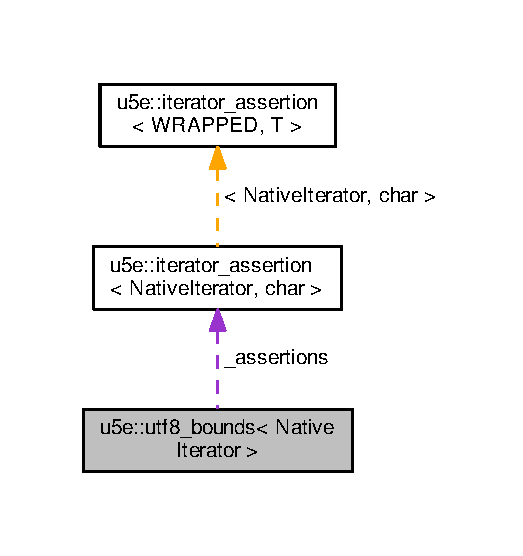
\includegraphics[width=251pt]{classu5e_1_1utf8__bounds__coll__graph}
\end{center}
\end{figure}
\subsection*{Static Public Member Functions}
\begin{DoxyCompactItemize}
\item 
static bool \hyperlink{classu5e_1_1utf8__bounds_aa694f7da507952fd82e19ade91e1e53e}{check} (Native\+Iterator begin, Native\+Iterator end)
\item 
static bool \hyperlink{classu5e_1_1utf8__bounds_ac46365c6e7895ed86e7ac54fb29ebda4}{enforce} (Native\+Iterator begin, Native\+Iterator end)
\end{DoxyCompactItemize}
\subsection*{Public Attributes}
\begin{DoxyCompactItemize}
\item 
\hyperlink{classu5e_1_1iterator__assertion}{iterator\+\_\+assertion}$<$ Native\+Iterator, char $>$ \hyperlink{classu5e_1_1utf8__bounds_a7469c5f9eaf73b8852039329279e3c0e}{\+\_\+assertions}
\end{DoxyCompactItemize}


\subsection{Detailed Description}
\subsubsection*{template$<$typename Native\+Iterator$>$\\*
class u5e\+::utf8\+\_\+bounds$<$ Native\+Iterator $>$}

Check and enforce bounds of \hyperlink{classu5e_1_1utf8}{utf8} text. 

This will only look at the last 6 octets of the text and will only look at the first octet. It will not guarantee that the entire text is valid. The intent of this class is to provide a cheap safety check to make sure you will not have any under or overflow when processing this text.


\begin{DoxyTemplParams}{Template Parameters}
{\em Native\+Iterator} & The native type to be iterated over. \\
\hline
\end{DoxyTemplParams}


Definition at line 21 of file utf8\+\_\+bounds.\+hpp.



\subsection{Member Function Documentation}
\index{u5e\+::utf8\+\_\+bounds@{u5e\+::utf8\+\_\+bounds}!check@{check}}
\index{check@{check}!u5e\+::utf8\+\_\+bounds@{u5e\+::utf8\+\_\+bounds}}
\subsubsection[{\texorpdfstring{check(\+Native\+Iterator begin, Native\+Iterator end)}{check(NativeIterator begin, NativeIterator end)}}]{\setlength{\rightskip}{0pt plus 5cm}template$<$typename Native\+Iterator $>$ static bool {\bf u5e\+::utf8\+\_\+bounds}$<$ Native\+Iterator $>$\+::check (
\begin{DoxyParamCaption}
\item[{Native\+Iterator}]{begin, }
\item[{Native\+Iterator}]{end}
\end{DoxyParamCaption}
)\hspace{0.3cm}{\ttfamily [inline]}, {\ttfamily [static]}}\hypertarget{classu5e_1_1utf8__bounds_aa694f7da507952fd82e19ade91e1e53e}{}\label{classu5e_1_1utf8__bounds_aa694f7da507952fd82e19ade91e1e53e}
Check the bounds of the \hyperlink{classu5e_1_1utf8}{utf8} text, returns true if the text has correct bounds. 

Definition at line 32 of file utf8\+\_\+bounds.\+hpp.

\index{u5e\+::utf8\+\_\+bounds@{u5e\+::utf8\+\_\+bounds}!enforce@{enforce}}
\index{enforce@{enforce}!u5e\+::utf8\+\_\+bounds@{u5e\+::utf8\+\_\+bounds}}
\subsubsection[{\texorpdfstring{enforce(\+Native\+Iterator begin, Native\+Iterator end)}{enforce(NativeIterator begin, NativeIterator end)}}]{\setlength{\rightskip}{0pt plus 5cm}template$<$typename Native\+Iterator $>$ static bool {\bf u5e\+::utf8\+\_\+bounds}$<$ Native\+Iterator $>$\+::enforce (
\begin{DoxyParamCaption}
\item[{Native\+Iterator}]{begin, }
\item[{Native\+Iterator}]{end}
\end{DoxyParamCaption}
)\hspace{0.3cm}{\ttfamily [inline]}, {\ttfamily [static]}}\hypertarget{classu5e_1_1utf8__bounds_ac46365c6e7895ed86e7ac54fb29ebda4}{}\label{classu5e_1_1utf8__bounds_ac46365c6e7895ed86e7ac54fb29ebda4}
Enforce the bounds of the \hyperlink{classu5e_1_1utf8}{utf8} text, replace any bad character in the bounds by \textquotesingle{}?. Returns false if any substitution was made. 

Definition at line 57 of file utf8\+\_\+bounds.\+hpp.



\subsection{Member Data Documentation}
\index{u5e\+::utf8\+\_\+bounds@{u5e\+::utf8\+\_\+bounds}!\+\_\+assertions@{\+\_\+assertions}}
\index{\+\_\+assertions@{\+\_\+assertions}!u5e\+::utf8\+\_\+bounds@{u5e\+::utf8\+\_\+bounds}}
\subsubsection[{\texorpdfstring{\+\_\+assertions}{_assertions}}]{\setlength{\rightskip}{0pt plus 5cm}template$<$typename Native\+Iterator $>$ {\bf iterator\+\_\+assertion}$<$Native\+Iterator, char$>$ {\bf u5e\+::utf8\+\_\+bounds}$<$ Native\+Iterator $>$\+::\+\_\+assertions}\hypertarget{classu5e_1_1utf8__bounds_a7469c5f9eaf73b8852039329279e3c0e}{}\label{classu5e_1_1utf8__bounds_a7469c5f9eaf73b8852039329279e3c0e}
The Native\+Iterator must match the attributes of char 

Definition at line 26 of file utf8\+\_\+bounds.\+hpp.



The documentation for this class was generated from the following file\+:\begin{DoxyCompactItemize}
\item 
u5e/utf8\+\_\+bounds.\+hpp\end{DoxyCompactItemize}

\hypertarget{classu5e_1_1utf8__const__iterator}{}\section{u5e\+:\+:utf8\+\_\+const\+\_\+iterator$<$ Native\+Iterator $>$ Class Template Reference}
\label{classu5e_1_1utf8__const__iterator}\index{u5e\+::utf8\+\_\+const\+\_\+iterator$<$ Native\+Iterator $>$@{u5e\+::utf8\+\_\+const\+\_\+iterator$<$ Native\+Iterator $>$}}


const iterator for \hyperlink{classu5e_1_1utf8}{utf8} encoded strings.  




{\ttfamily \#include $<$u5e/utf8\+\_\+iterator.\+hpp$>$}



Inheritance diagram for u5e\+:\+:utf8\+\_\+const\+\_\+iterator$<$ Native\+Iterator $>$\+:
\nopagebreak
\begin{figure}[H]
\begin{center}
\leavevmode
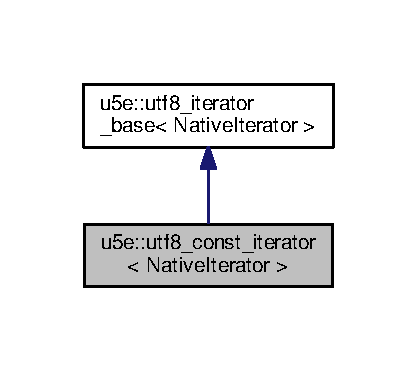
\includegraphics[width=200pt]{classu5e_1_1utf8__const__iterator__inherit__graph}
\end{center}
\end{figure}


Collaboration diagram for u5e\+:\+:utf8\+\_\+const\+\_\+iterator$<$ Native\+Iterator $>$\+:
\nopagebreak
\begin{figure}[H]
\begin{center}
\leavevmode
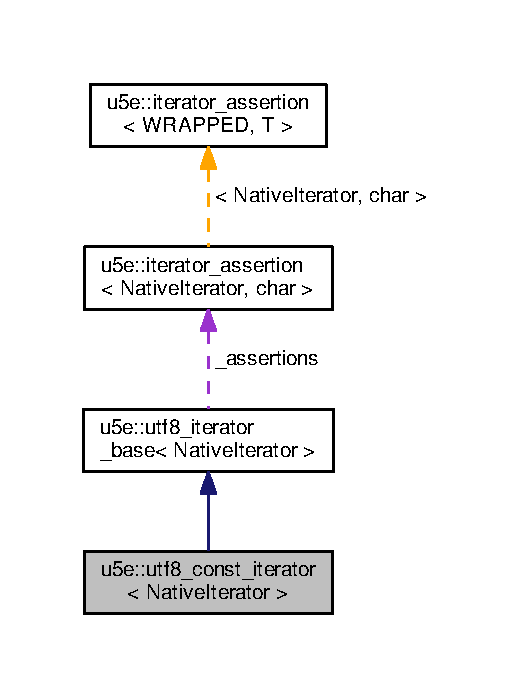
\includegraphics[width=246pt]{classu5e_1_1utf8__const__iterator__coll__graph}
\end{center}
\end{figure}
\subsection*{Public Types}
\begin{DoxyCompactItemize}
\item 
typedef \hyperlink{classu5e_1_1utf8__const__iterator}{utf8\+\_\+const\+\_\+iterator} \hyperlink{classu5e_1_1utf8__const__iterator_ab8b6bc6c6b56d00ff1a8b9a896be6f3f}{pointer}
\end{DoxyCompactItemize}
\subsection*{Public Member Functions}
\begin{DoxyCompactItemize}
\item 
\hyperlink{classu5e_1_1utf8__const__iterator_a63fa9eebf92db15410ba8864208ebb82}{utf8\+\_\+const\+\_\+iterator} (const Native\+Iterator raw\+\_\+iterator)
\item 
\hyperlink{classu5e_1_1utf8__const__iterator_a7beaaaf0bf9784170014b868e060b091}{utf8\+\_\+const\+\_\+iterator} (const \hyperlink{classu5e_1_1utf8__const__iterator}{utf8\+\_\+const\+\_\+iterator} \&tocopy)
\item 
const \hyperlink{classu5e_1_1codepoint}{codepoint} \hyperlink{classu5e_1_1utf8__const__iterator_addd93a5294e3ba66ab82d2ca6f5d87be}{operator$\ast$} ()
\end{DoxyCompactItemize}
{\bf }\par
\begin{DoxyCompactItemize}
\item 
\hyperlink{classu5e_1_1utf8__const__iterator}{utf8\+\_\+const\+\_\+iterator} \& \hyperlink{classu5e_1_1utf8__const__iterator_a6012ac7067df6be5b84cad638cc9b13c}{operator++} ()
\item 
\hyperlink{classu5e_1_1utf8__const__iterator}{utf8\+\_\+const\+\_\+iterator} \hyperlink{classu5e_1_1utf8__const__iterator_a1449b50f26f761993e382bb93a8736db}{operator++} (int junk)
\end{DoxyCompactItemize}

{\bf }\par
\begin{DoxyCompactItemize}
\item 
\hyperlink{classu5e_1_1utf8__const__iterator}{utf8\+\_\+const\+\_\+iterator} \& \hyperlink{classu5e_1_1utf8__const__iterator_a5fdcd90a37a0aa4a3444c7b12dc46765}{operator-\/-\/} ()
\item 
\hyperlink{classu5e_1_1utf8__const__iterator}{utf8\+\_\+const\+\_\+iterator} \hyperlink{classu5e_1_1utf8__const__iterator_aefe09be687e582d4132ca3e3ee4b59dd}{operator-\/-\/} (int junk)
\end{DoxyCompactItemize}

{\bf }\par
\begin{DoxyCompactItemize}
\item 
bool \hyperlink{classu5e_1_1utf8__const__iterator_ac6110586d118a41b5eeac023f4788ccb}{operator==} (const \hyperlink{classu5e_1_1utf8__const__iterator}{utf8\+\_\+const\+\_\+iterator} \&rhs) const 
\item 
bool \hyperlink{classu5e_1_1utf8__const__iterator_a776a1dae46835c0871a945c0da418498}{operator!=} (const \hyperlink{classu5e_1_1utf8__const__iterator}{utf8\+\_\+const\+\_\+iterator} \&rhs) const 
\end{DoxyCompactItemize}

\subsection*{Additional Inherited Members}


\subsection{Detailed Description}
\subsubsection*{template$<$typename Native\+Iterator$>$\\*
class u5e\+::utf8\+\_\+const\+\_\+iterator$<$ Native\+Iterator $>$}

const iterator for \hyperlink{classu5e_1_1utf8}{utf8} encoded strings. 


\begin{DoxyTemplParams}{Template Parameters}
{\em Native\+Iterator} & The underlying type to be iterated over. \\
\hline
\end{DoxyTemplParams}


Definition at line 110 of file utf8\+\_\+iterator.\+hpp.



\subsection{Member Typedef Documentation}
\index{u5e\+::utf8\+\_\+const\+\_\+iterator@{u5e\+::utf8\+\_\+const\+\_\+iterator}!pointer@{pointer}}
\index{pointer@{pointer}!u5e\+::utf8\+\_\+const\+\_\+iterator@{u5e\+::utf8\+\_\+const\+\_\+iterator}}
\subsubsection[{\texorpdfstring{pointer}{pointer}}]{\setlength{\rightskip}{0pt plus 5cm}template$<$typename Native\+Iterator $>$ typedef {\bf utf8\+\_\+const\+\_\+iterator} {\bf u5e\+::utf8\+\_\+const\+\_\+iterator}$<$ Native\+Iterator $>$\+::{\bf pointer}}\hypertarget{classu5e_1_1utf8__const__iterator_ab8b6bc6c6b56d00ff1a8b9a896be6f3f}{}\label{classu5e_1_1utf8__const__iterator_ab8b6bc6c6b56d00ff1a8b9a896be6f3f}
Offers itself as the pointer type 

Definition at line 116 of file utf8\+\_\+iterator.\+hpp.



\subsection{Constructor \& Destructor Documentation}
\index{u5e\+::utf8\+\_\+const\+\_\+iterator@{u5e\+::utf8\+\_\+const\+\_\+iterator}!utf8\+\_\+const\+\_\+iterator@{utf8\+\_\+const\+\_\+iterator}}
\index{utf8\+\_\+const\+\_\+iterator@{utf8\+\_\+const\+\_\+iterator}!u5e\+::utf8\+\_\+const\+\_\+iterator@{u5e\+::utf8\+\_\+const\+\_\+iterator}}
\subsubsection[{\texorpdfstring{utf8\+\_\+const\+\_\+iterator(const Native\+Iterator raw\+\_\+iterator)}{utf8_const_iterator(const NativeIterator raw_iterator)}}]{\setlength{\rightskip}{0pt plus 5cm}template$<$typename Native\+Iterator $>$ {\bf u5e\+::utf8\+\_\+const\+\_\+iterator}$<$ Native\+Iterator $>$\+::{\bf utf8\+\_\+const\+\_\+iterator} (
\begin{DoxyParamCaption}
\item[{const Native\+Iterator}]{raw\+\_\+iterator}
\end{DoxyParamCaption}
)\hspace{0.3cm}{\ttfamily [inline]}}\hypertarget{classu5e_1_1utf8__const__iterator_a63fa9eebf92db15410ba8864208ebb82}{}\label{classu5e_1_1utf8__const__iterator_a63fa9eebf92db15410ba8864208ebb82}
Create from the underlying iterator type 

Definition at line 121 of file utf8\+\_\+iterator.\+hpp.

\index{u5e\+::utf8\+\_\+const\+\_\+iterator@{u5e\+::utf8\+\_\+const\+\_\+iterator}!utf8\+\_\+const\+\_\+iterator@{utf8\+\_\+const\+\_\+iterator}}
\index{utf8\+\_\+const\+\_\+iterator@{utf8\+\_\+const\+\_\+iterator}!u5e\+::utf8\+\_\+const\+\_\+iterator@{u5e\+::utf8\+\_\+const\+\_\+iterator}}
\subsubsection[{\texorpdfstring{utf8\+\_\+const\+\_\+iterator(const utf8\+\_\+const\+\_\+iterator \&tocopy)}{utf8_const_iterator(const utf8_const_iterator &tocopy)}}]{\setlength{\rightskip}{0pt plus 5cm}template$<$typename Native\+Iterator $>$ {\bf u5e\+::utf8\+\_\+const\+\_\+iterator}$<$ Native\+Iterator $>$\+::{\bf utf8\+\_\+const\+\_\+iterator} (
\begin{DoxyParamCaption}
\item[{const {\bf utf8\+\_\+const\+\_\+iterator}$<$ Native\+Iterator $>$ \&}]{tocopy}
\end{DoxyParamCaption}
)\hspace{0.3cm}{\ttfamily [inline]}}\hypertarget{classu5e_1_1utf8__const__iterator_a7beaaaf0bf9784170014b868e060b091}{}\label{classu5e_1_1utf8__const__iterator_a7beaaaf0bf9784170014b868e060b091}
Copy constructor 

Definition at line 127 of file utf8\+\_\+iterator.\+hpp.



\subsection{Member Function Documentation}
\index{u5e\+::utf8\+\_\+const\+\_\+iterator@{u5e\+::utf8\+\_\+const\+\_\+iterator}!operator"!=@{operator"!=}}
\index{operator"!=@{operator"!=}!u5e\+::utf8\+\_\+const\+\_\+iterator@{u5e\+::utf8\+\_\+const\+\_\+iterator}}
\subsubsection[{\texorpdfstring{operator"!=(const utf8\+\_\+const\+\_\+iterator \&rhs) const }{operator!=(const utf8_const_iterator &rhs) const }}]{\setlength{\rightskip}{0pt plus 5cm}template$<$typename Native\+Iterator $>$ bool {\bf u5e\+::utf8\+\_\+const\+\_\+iterator}$<$ Native\+Iterator $>$\+::operator!= (
\begin{DoxyParamCaption}
\item[{const {\bf utf8\+\_\+const\+\_\+iterator}$<$ Native\+Iterator $>$ \&}]{rhs}
\end{DoxyParamCaption}
) const\hspace{0.3cm}{\ttfamily [inline]}}\hypertarget{classu5e_1_1utf8__const__iterator_a776a1dae46835c0871a945c0da418498}{}\label{classu5e_1_1utf8__const__iterator_a776a1dae46835c0871a945c0da418498}
Compare with another iterator 

Definition at line 183 of file utf8\+\_\+iterator.\+hpp.

\index{u5e\+::utf8\+\_\+const\+\_\+iterator@{u5e\+::utf8\+\_\+const\+\_\+iterator}!operator$\ast$@{operator$\ast$}}
\index{operator$\ast$@{operator$\ast$}!u5e\+::utf8\+\_\+const\+\_\+iterator@{u5e\+::utf8\+\_\+const\+\_\+iterator}}
\subsubsection[{\texorpdfstring{operator$\ast$()}{operator*()}}]{\setlength{\rightskip}{0pt plus 5cm}template$<$typename Native\+Iterator $>$ const {\bf codepoint} {\bf u5e\+::utf8\+\_\+const\+\_\+iterator}$<$ Native\+Iterator $>$\+::operator$\ast$ (
\begin{DoxyParamCaption}
{}
\end{DoxyParamCaption}
)\hspace{0.3cm}{\ttfamily [inline]}}\hypertarget{classu5e_1_1utf8__const__iterator_addd93a5294e3ba66ab82d2ca6f5d87be}{}\label{classu5e_1_1utf8__const__iterator_addd93a5294e3ba66ab82d2ca6f5d87be}
Dereference the current codepoint out of the iterator 

Definition at line 191 of file utf8\+\_\+iterator.\+hpp.

\index{u5e\+::utf8\+\_\+const\+\_\+iterator@{u5e\+::utf8\+\_\+const\+\_\+iterator}!operator++@{operator++}}
\index{operator++@{operator++}!u5e\+::utf8\+\_\+const\+\_\+iterator@{u5e\+::utf8\+\_\+const\+\_\+iterator}}
\subsubsection[{\texorpdfstring{operator++()}{operator++()}}]{\setlength{\rightskip}{0pt plus 5cm}template$<$typename Native\+Iterator $>$ {\bf utf8\+\_\+const\+\_\+iterator}\& {\bf u5e\+::utf8\+\_\+const\+\_\+iterator}$<$ Native\+Iterator $>$\+::operator++ (
\begin{DoxyParamCaption}
{}
\end{DoxyParamCaption}
)\hspace{0.3cm}{\ttfamily [inline]}}\hypertarget{classu5e_1_1utf8__const__iterator_a6012ac7067df6be5b84cad638cc9b13c}{}\label{classu5e_1_1utf8__const__iterator_a6012ac7067df6be5b84cad638cc9b13c}
Advance the iterator 

Definition at line 134 of file utf8\+\_\+iterator.\+hpp.

\index{u5e\+::utf8\+\_\+const\+\_\+iterator@{u5e\+::utf8\+\_\+const\+\_\+iterator}!operator++@{operator++}}
\index{operator++@{operator++}!u5e\+::utf8\+\_\+const\+\_\+iterator@{u5e\+::utf8\+\_\+const\+\_\+iterator}}
\subsubsection[{\texorpdfstring{operator++(int junk)}{operator++(int junk)}}]{\setlength{\rightskip}{0pt plus 5cm}template$<$typename Native\+Iterator $>$ {\bf utf8\+\_\+const\+\_\+iterator} {\bf u5e\+::utf8\+\_\+const\+\_\+iterator}$<$ Native\+Iterator $>$\+::operator++ (
\begin{DoxyParamCaption}
\item[{int}]{junk}
\end{DoxyParamCaption}
)\hspace{0.3cm}{\ttfamily [inline]}}\hypertarget{classu5e_1_1utf8__const__iterator_a1449b50f26f761993e382bb93a8736db}{}\label{classu5e_1_1utf8__const__iterator_a1449b50f26f761993e382bb93a8736db}
Advance the iterator 

Definition at line 139 of file utf8\+\_\+iterator.\+hpp.

\index{u5e\+::utf8\+\_\+const\+\_\+iterator@{u5e\+::utf8\+\_\+const\+\_\+iterator}!operator-\/-\/@{operator-\/-\/}}
\index{operator-\/-\/@{operator-\/-\/}!u5e\+::utf8\+\_\+const\+\_\+iterator@{u5e\+::utf8\+\_\+const\+\_\+iterator}}
\subsubsection[{\texorpdfstring{operator-\/-\/()}{operator--()}}]{\setlength{\rightskip}{0pt plus 5cm}template$<$typename Native\+Iterator $>$ {\bf utf8\+\_\+const\+\_\+iterator}\& {\bf u5e\+::utf8\+\_\+const\+\_\+iterator}$<$ Native\+Iterator $>$\+::operator-\/-\/ (
\begin{DoxyParamCaption}
{}
\end{DoxyParamCaption}
)\hspace{0.3cm}{\ttfamily [inline]}}\hypertarget{classu5e_1_1utf8__const__iterator_a5fdcd90a37a0aa4a3444c7b12dc46765}{}\label{classu5e_1_1utf8__const__iterator_a5fdcd90a37a0aa4a3444c7b12dc46765}
Rewinds the iterator 

Definition at line 150 of file utf8\+\_\+iterator.\+hpp.

\index{u5e\+::utf8\+\_\+const\+\_\+iterator@{u5e\+::utf8\+\_\+const\+\_\+iterator}!operator-\/-\/@{operator-\/-\/}}
\index{operator-\/-\/@{operator-\/-\/}!u5e\+::utf8\+\_\+const\+\_\+iterator@{u5e\+::utf8\+\_\+const\+\_\+iterator}}
\subsubsection[{\texorpdfstring{operator-\/-\/(int junk)}{operator--(int junk)}}]{\setlength{\rightskip}{0pt plus 5cm}template$<$typename Native\+Iterator $>$ {\bf utf8\+\_\+const\+\_\+iterator} {\bf u5e\+::utf8\+\_\+const\+\_\+iterator}$<$ Native\+Iterator $>$\+::operator-\/-\/ (
\begin{DoxyParamCaption}
\item[{int}]{junk}
\end{DoxyParamCaption}
)\hspace{0.3cm}{\ttfamily [inline]}}\hypertarget{classu5e_1_1utf8__const__iterator_aefe09be687e582d4132ca3e3ee4b59dd}{}\label{classu5e_1_1utf8__const__iterator_aefe09be687e582d4132ca3e3ee4b59dd}
Rewinds the iterator 

Definition at line 155 of file utf8\+\_\+iterator.\+hpp.

\index{u5e\+::utf8\+\_\+const\+\_\+iterator@{u5e\+::utf8\+\_\+const\+\_\+iterator}!operator==@{operator==}}
\index{operator==@{operator==}!u5e\+::utf8\+\_\+const\+\_\+iterator@{u5e\+::utf8\+\_\+const\+\_\+iterator}}
\subsubsection[{\texorpdfstring{operator==(const utf8\+\_\+const\+\_\+iterator \&rhs) const }{operator==(const utf8_const_iterator &rhs) const }}]{\setlength{\rightskip}{0pt plus 5cm}template$<$typename Native\+Iterator $>$ bool {\bf u5e\+::utf8\+\_\+const\+\_\+iterator}$<$ Native\+Iterator $>$\+::operator== (
\begin{DoxyParamCaption}
\item[{const {\bf utf8\+\_\+const\+\_\+iterator}$<$ Native\+Iterator $>$ \&}]{rhs}
\end{DoxyParamCaption}
) const\hspace{0.3cm}{\ttfamily [inline]}}\hypertarget{classu5e_1_1utf8__const__iterator_ac6110586d118a41b5eeac023f4788ccb}{}\label{classu5e_1_1utf8__const__iterator_ac6110586d118a41b5eeac023f4788ccb}
Compare with another iterator 

Definition at line 166 of file utf8\+\_\+iterator.\+hpp.



The documentation for this class was generated from the following file\+:\begin{DoxyCompactItemize}
\item 
u5e/utf8\+\_\+iterator.\+hpp\end{DoxyCompactItemize}

\hypertarget{classu5e_1_1utf8__iterator}{}\section{u5e\+:\+:utf8\+\_\+iterator$<$ Native\+Iterator $>$ Class Template Reference}
\label{classu5e_1_1utf8__iterator}\index{u5e\+::utf8\+\_\+iterator$<$ Native\+Iterator $>$@{u5e\+::utf8\+\_\+iterator$<$ Native\+Iterator $>$}}


mutable \hyperlink{classu5e_1_1utf8}{utf8} iterator  




{\ttfamily \#include $<$u5e/utf8\+\_\+iterator.\+hpp$>$}



Inheritance diagram for u5e\+:\+:utf8\+\_\+iterator$<$ Native\+Iterator $>$\+:
\nopagebreak
\begin{figure}[H]
\begin{center}
\leavevmode
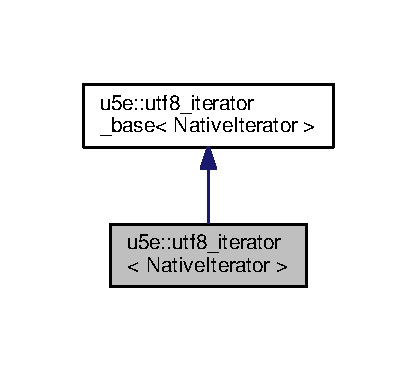
\includegraphics[width=200pt]{classu5e_1_1utf8__iterator__inherit__graph}
\end{center}
\end{figure}


Collaboration diagram for u5e\+:\+:utf8\+\_\+iterator$<$ Native\+Iterator $>$\+:
\nopagebreak
\begin{figure}[H]
\begin{center}
\leavevmode
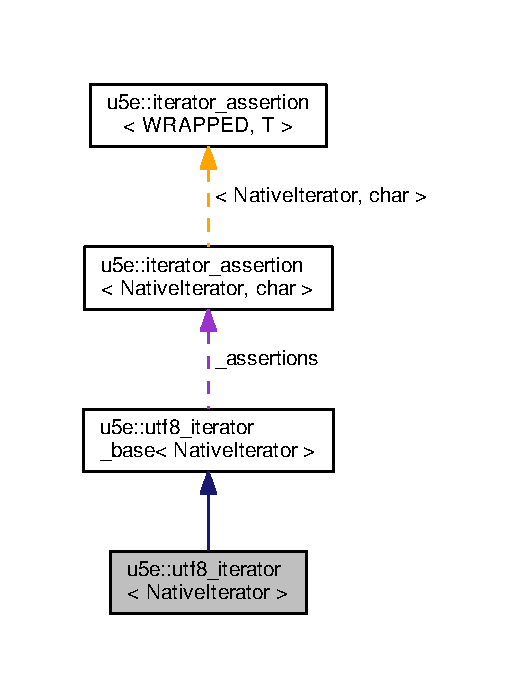
\includegraphics[width=246pt]{classu5e_1_1utf8__iterator__coll__graph}
\end{center}
\end{figure}
\subsection*{Classes}
\begin{DoxyCompactItemize}
\item 
class \hyperlink{classu5e_1_1utf8__iterator_1_1proxyobject}{proxyobject}
\begin{DoxyCompactList}\small\item\em offers write access to the iterator at a given position \end{DoxyCompactList}\end{DoxyCompactItemize}
\subsection*{Public Types}
\begin{DoxyCompactItemize}
\item 
typedef \hyperlink{classu5e_1_1utf8__iterator}{utf8\+\_\+iterator} \hyperlink{classu5e_1_1utf8__iterator_a7f50a43350790b6f213e83427f8bb8b7}{pointer}
\end{DoxyCompactItemize}
\subsection*{Public Member Functions}
\begin{DoxyCompactItemize}
\item 
\hyperlink{classu5e_1_1utf8__iterator_ad50264ff5f219e7d7606c7b4d4bf8a3b}{utf8\+\_\+iterator} (const Native\+Iterator raw\+\_\+iterator)
\item 
\hyperlink{classu5e_1_1utf8__iterator_acea20d0f74e2cd7f04d7b6f5e41a2e18}{utf8\+\_\+iterator} (const \hyperlink{classu5e_1_1utf8__iterator}{utf8\+\_\+iterator} \&tocopy)
\item 
\hyperlink{classu5e_1_1utf8__iterator_1_1proxyobject}{proxyobject} \hyperlink{classu5e_1_1utf8__iterator_acdfcb12b677372e6ff72b72740f489e4}{operator$\ast$} ()
\end{DoxyCompactItemize}
{\bf }\par
\begin{DoxyCompactItemize}
\item 
\hyperlink{classu5e_1_1utf8__iterator}{utf8\+\_\+iterator} \& \hyperlink{classu5e_1_1utf8__iterator_ab6431e6ba7010f9fd7a1eba079022781}{operator++} ()
\item 
\hyperlink{classu5e_1_1utf8__iterator}{utf8\+\_\+iterator} \hyperlink{classu5e_1_1utf8__iterator_a13fba9b49f844b9b1929e46a9bb8d4e8}{operator++} (int junk)
\end{DoxyCompactItemize}

{\bf }\par
\begin{DoxyCompactItemize}
\item 
\hyperlink{classu5e_1_1utf8__iterator}{utf8\+\_\+iterator} \& \hyperlink{classu5e_1_1utf8__iterator_a861465404fbc47279b05af200372484d}{operator-\/-\/} ()
\item 
\hyperlink{classu5e_1_1utf8__iterator}{utf8\+\_\+iterator} \hyperlink{classu5e_1_1utf8__iterator_a96fb0763063cb54e94fac8c201f7367d}{operator-\/-\/} (int junk)
\end{DoxyCompactItemize}

{\bf }\par
\begin{DoxyCompactItemize}
\item 
bool \hyperlink{classu5e_1_1utf8__iterator_a8a19d76a5cff4853f4f281bc330c00e6}{operator==} (const \hyperlink{classu5e_1_1utf8__iterator}{utf8\+\_\+iterator} \&rhs) const 
\item 
bool \hyperlink{classu5e_1_1utf8__iterator_a64020160892753ed7628728836bc9555}{operator!=} (const \hyperlink{classu5e_1_1utf8__iterator}{utf8\+\_\+iterator} \&rhs) const 
\end{DoxyCompactItemize}

\subsection*{Additional Inherited Members}


\subsection{Detailed Description}
\subsubsection*{template$<$typename Native\+Iterator$>$\\*
class u5e\+::utf8\+\_\+iterator$<$ Native\+Iterator $>$}

mutable \hyperlink{classu5e_1_1utf8}{utf8} iterator 

Note that if you set a value in the middle of a text, you will likely make the string invalid. Most of the time you should only consider appending to an iterator, never writing in the middle of the text. 
\begin{DoxyTemplParams}{Template Parameters}
{\em Native\+Iterator} & The underlying type to be iterated over. \\
\hline
\end{DoxyTemplParams}


Definition at line 207 of file utf8\+\_\+iterator.\+hpp.



\subsection{Member Typedef Documentation}
\index{u5e\+::utf8\+\_\+iterator@{u5e\+::utf8\+\_\+iterator}!pointer@{pointer}}
\index{pointer@{pointer}!u5e\+::utf8\+\_\+iterator@{u5e\+::utf8\+\_\+iterator}}
\subsubsection[{\texorpdfstring{pointer}{pointer}}]{\setlength{\rightskip}{0pt plus 5cm}template$<$typename Native\+Iterator$>$ typedef {\bf utf8\+\_\+iterator} {\bf u5e\+::utf8\+\_\+iterator}$<$ Native\+Iterator $>$\+::{\bf pointer}}\hypertarget{classu5e_1_1utf8__iterator_a7f50a43350790b6f213e83427f8bb8b7}{}\label{classu5e_1_1utf8__iterator_a7f50a43350790b6f213e83427f8bb8b7}
Offer itself as the pointer type 

Definition at line 213 of file utf8\+\_\+iterator.\+hpp.



\subsection{Constructor \& Destructor Documentation}
\index{u5e\+::utf8\+\_\+iterator@{u5e\+::utf8\+\_\+iterator}!utf8\+\_\+iterator@{utf8\+\_\+iterator}}
\index{utf8\+\_\+iterator@{utf8\+\_\+iterator}!u5e\+::utf8\+\_\+iterator@{u5e\+::utf8\+\_\+iterator}}
\subsubsection[{\texorpdfstring{utf8\+\_\+iterator(const Native\+Iterator raw\+\_\+iterator)}{utf8_iterator(const NativeIterator raw_iterator)}}]{\setlength{\rightskip}{0pt plus 5cm}template$<$typename Native\+Iterator$>$ {\bf u5e\+::utf8\+\_\+iterator}$<$ Native\+Iterator $>$\+::{\bf utf8\+\_\+iterator} (
\begin{DoxyParamCaption}
\item[{const Native\+Iterator}]{raw\+\_\+iterator}
\end{DoxyParamCaption}
)\hspace{0.3cm}{\ttfamily [inline]}}\hypertarget{classu5e_1_1utf8__iterator_ad50264ff5f219e7d7606c7b4d4bf8a3b}{}\label{classu5e_1_1utf8__iterator_ad50264ff5f219e7d7606c7b4d4bf8a3b}
Construct fro the underlying iterator 

Definition at line 218 of file utf8\+\_\+iterator.\+hpp.

\index{u5e\+::utf8\+\_\+iterator@{u5e\+::utf8\+\_\+iterator}!utf8\+\_\+iterator@{utf8\+\_\+iterator}}
\index{utf8\+\_\+iterator@{utf8\+\_\+iterator}!u5e\+::utf8\+\_\+iterator@{u5e\+::utf8\+\_\+iterator}}
\subsubsection[{\texorpdfstring{utf8\+\_\+iterator(const utf8\+\_\+iterator \&tocopy)}{utf8_iterator(const utf8_iterator &tocopy)}}]{\setlength{\rightskip}{0pt plus 5cm}template$<$typename Native\+Iterator$>$ {\bf u5e\+::utf8\+\_\+iterator}$<$ Native\+Iterator $>$\+::{\bf utf8\+\_\+iterator} (
\begin{DoxyParamCaption}
\item[{const {\bf utf8\+\_\+iterator}$<$ Native\+Iterator $>$ \&}]{tocopy}
\end{DoxyParamCaption}
)\hspace{0.3cm}{\ttfamily [inline]}}\hypertarget{classu5e_1_1utf8__iterator_acea20d0f74e2cd7f04d7b6f5e41a2e18}{}\label{classu5e_1_1utf8__iterator_acea20d0f74e2cd7f04d7b6f5e41a2e18}
Copy constructor 

Definition at line 224 of file utf8\+\_\+iterator.\+hpp.



\subsection{Member Function Documentation}
\index{u5e\+::utf8\+\_\+iterator@{u5e\+::utf8\+\_\+iterator}!operator"!=@{operator"!=}}
\index{operator"!=@{operator"!=}!u5e\+::utf8\+\_\+iterator@{u5e\+::utf8\+\_\+iterator}}
\subsubsection[{\texorpdfstring{operator"!=(const utf8\+\_\+iterator \&rhs) const }{operator!=(const utf8_iterator &rhs) const }}]{\setlength{\rightskip}{0pt plus 5cm}template$<$typename Native\+Iterator$>$ bool {\bf u5e\+::utf8\+\_\+iterator}$<$ Native\+Iterator $>$\+::operator!= (
\begin{DoxyParamCaption}
\item[{const {\bf utf8\+\_\+iterator}$<$ Native\+Iterator $>$ \&}]{rhs}
\end{DoxyParamCaption}
) const\hspace{0.3cm}{\ttfamily [inline]}}\hypertarget{classu5e_1_1utf8__iterator_a64020160892753ed7628728836bc9555}{}\label{classu5e_1_1utf8__iterator_a64020160892753ed7628728836bc9555}
Compare the iterator with another iterator 

Definition at line 280 of file utf8\+\_\+iterator.\+hpp.

\index{u5e\+::utf8\+\_\+iterator@{u5e\+::utf8\+\_\+iterator}!operator$\ast$@{operator$\ast$}}
\index{operator$\ast$@{operator$\ast$}!u5e\+::utf8\+\_\+iterator@{u5e\+::utf8\+\_\+iterator}}
\subsubsection[{\texorpdfstring{operator$\ast$()}{operator*()}}]{\setlength{\rightskip}{0pt plus 5cm}template$<$typename Native\+Iterator$>$ {\bf proxyobject} {\bf u5e\+::utf8\+\_\+iterator}$<$ Native\+Iterator $>$\+::operator$\ast$ (
\begin{DoxyParamCaption}
{}
\end{DoxyParamCaption}
)\hspace{0.3cm}{\ttfamily [inline]}}\hypertarget{classu5e_1_1utf8__iterator_acdfcb12b677372e6ff72b72740f489e4}{}\label{classu5e_1_1utf8__iterator_acdfcb12b677372e6ff72b72740f489e4}
mutable \hyperlink{classu5e_1_1utf8}{utf8} iterator returns a proxy object in order to allow assignment to happen. 

Definition at line 340 of file utf8\+\_\+iterator.\+hpp.

\index{u5e\+::utf8\+\_\+iterator@{u5e\+::utf8\+\_\+iterator}!operator++@{operator++}}
\index{operator++@{operator++}!u5e\+::utf8\+\_\+iterator@{u5e\+::utf8\+\_\+iterator}}
\subsubsection[{\texorpdfstring{operator++()}{operator++()}}]{\setlength{\rightskip}{0pt plus 5cm}template$<$typename Native\+Iterator$>$ {\bf utf8\+\_\+iterator}\& {\bf u5e\+::utf8\+\_\+iterator}$<$ Native\+Iterator $>$\+::operator++ (
\begin{DoxyParamCaption}
{}
\end{DoxyParamCaption}
)\hspace{0.3cm}{\ttfamily [inline]}}\hypertarget{classu5e_1_1utf8__iterator_ab6431e6ba7010f9fd7a1eba079022781}{}\label{classu5e_1_1utf8__iterator_ab6431e6ba7010f9fd7a1eba079022781}
Advance the iterator 

Definition at line 231 of file utf8\+\_\+iterator.\+hpp.

\index{u5e\+::utf8\+\_\+iterator@{u5e\+::utf8\+\_\+iterator}!operator++@{operator++}}
\index{operator++@{operator++}!u5e\+::utf8\+\_\+iterator@{u5e\+::utf8\+\_\+iterator}}
\subsubsection[{\texorpdfstring{operator++(int junk)}{operator++(int junk)}}]{\setlength{\rightskip}{0pt plus 5cm}template$<$typename Native\+Iterator$>$ {\bf utf8\+\_\+iterator} {\bf u5e\+::utf8\+\_\+iterator}$<$ Native\+Iterator $>$\+::operator++ (
\begin{DoxyParamCaption}
\item[{int}]{junk}
\end{DoxyParamCaption}
)\hspace{0.3cm}{\ttfamily [inline]}}\hypertarget{classu5e_1_1utf8__iterator_a13fba9b49f844b9b1929e46a9bb8d4e8}{}\label{classu5e_1_1utf8__iterator_a13fba9b49f844b9b1929e46a9bb8d4e8}
Advance the iterator 

Definition at line 236 of file utf8\+\_\+iterator.\+hpp.

\index{u5e\+::utf8\+\_\+iterator@{u5e\+::utf8\+\_\+iterator}!operator-\/-\/@{operator-\/-\/}}
\index{operator-\/-\/@{operator-\/-\/}!u5e\+::utf8\+\_\+iterator@{u5e\+::utf8\+\_\+iterator}}
\subsubsection[{\texorpdfstring{operator-\/-\/()}{operator--()}}]{\setlength{\rightskip}{0pt plus 5cm}template$<$typename Native\+Iterator$>$ {\bf utf8\+\_\+iterator}\& {\bf u5e\+::utf8\+\_\+iterator}$<$ Native\+Iterator $>$\+::operator-\/-\/ (
\begin{DoxyParamCaption}
{}
\end{DoxyParamCaption}
)\hspace{0.3cm}{\ttfamily [inline]}}\hypertarget{classu5e_1_1utf8__iterator_a861465404fbc47279b05af200372484d}{}\label{classu5e_1_1utf8__iterator_a861465404fbc47279b05af200372484d}
Rewind the iterator 

Definition at line 247 of file utf8\+\_\+iterator.\+hpp.

\index{u5e\+::utf8\+\_\+iterator@{u5e\+::utf8\+\_\+iterator}!operator-\/-\/@{operator-\/-\/}}
\index{operator-\/-\/@{operator-\/-\/}!u5e\+::utf8\+\_\+iterator@{u5e\+::utf8\+\_\+iterator}}
\subsubsection[{\texorpdfstring{operator-\/-\/(int junk)}{operator--(int junk)}}]{\setlength{\rightskip}{0pt plus 5cm}template$<$typename Native\+Iterator$>$ {\bf utf8\+\_\+iterator} {\bf u5e\+::utf8\+\_\+iterator}$<$ Native\+Iterator $>$\+::operator-\/-\/ (
\begin{DoxyParamCaption}
\item[{int}]{junk}
\end{DoxyParamCaption}
)\hspace{0.3cm}{\ttfamily [inline]}}\hypertarget{classu5e_1_1utf8__iterator_a96fb0763063cb54e94fac8c201f7367d}{}\label{classu5e_1_1utf8__iterator_a96fb0763063cb54e94fac8c201f7367d}
Rewind the iterator 

Definition at line 252 of file utf8\+\_\+iterator.\+hpp.

\index{u5e\+::utf8\+\_\+iterator@{u5e\+::utf8\+\_\+iterator}!operator==@{operator==}}
\index{operator==@{operator==}!u5e\+::utf8\+\_\+iterator@{u5e\+::utf8\+\_\+iterator}}
\subsubsection[{\texorpdfstring{operator==(const utf8\+\_\+iterator \&rhs) const }{operator==(const utf8_iterator &rhs) const }}]{\setlength{\rightskip}{0pt plus 5cm}template$<$typename Native\+Iterator$>$ bool {\bf u5e\+::utf8\+\_\+iterator}$<$ Native\+Iterator $>$\+::operator== (
\begin{DoxyParamCaption}
\item[{const {\bf utf8\+\_\+iterator}$<$ Native\+Iterator $>$ \&}]{rhs}
\end{DoxyParamCaption}
) const\hspace{0.3cm}{\ttfamily [inline]}}\hypertarget{classu5e_1_1utf8__iterator_a8a19d76a5cff4853f4f281bc330c00e6}{}\label{classu5e_1_1utf8__iterator_a8a19d76a5cff4853f4f281bc330c00e6}
Compare the iterator with another iterator 

Definition at line 263 of file utf8\+\_\+iterator.\+hpp.



The documentation for this class was generated from the following file\+:\begin{DoxyCompactItemize}
\item 
u5e/utf8\+\_\+iterator.\+hpp\end{DoxyCompactItemize}

\hypertarget{classu5e_1_1utf8__iterator__base}{}\section{u5e\+:\+:utf8\+\_\+iterator\+\_\+base$<$ Native\+Iterator $>$ Class Template Reference}
\label{classu5e_1_1utf8__iterator__base}\index{u5e\+::utf8\+\_\+iterator\+\_\+base$<$ Native\+Iterator $>$@{u5e\+::utf8\+\_\+iterator\+\_\+base$<$ Native\+Iterator $>$}}


Defines the basic inner workings of \hyperlink{classu5e_1_1utf8}{utf8} iterator.  




{\ttfamily \#include $<$u5e/utf8\+\_\+iterator.\+hpp$>$}



Inheritance diagram for u5e\+:\+:utf8\+\_\+iterator\+\_\+base$<$ Native\+Iterator $>$\+:
\nopagebreak
\begin{figure}[H]
\begin{center}
\leavevmode
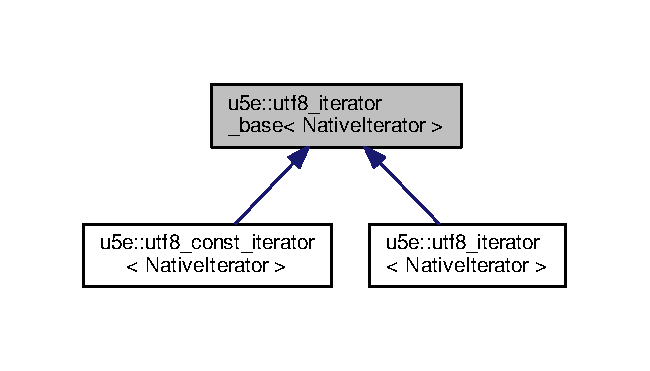
\includegraphics[width=312pt]{classu5e_1_1utf8__iterator__base__inherit__graph}
\end{center}
\end{figure}


Collaboration diagram for u5e\+:\+:utf8\+\_\+iterator\+\_\+base$<$ Native\+Iterator $>$\+:
\nopagebreak
\begin{figure}[H]
\begin{center}
\leavevmode
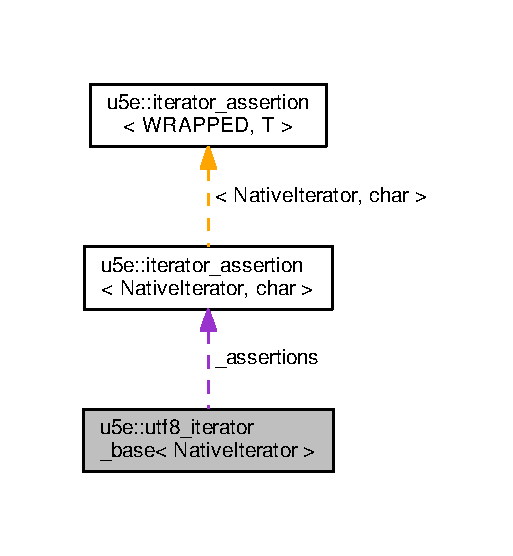
\includegraphics[width=246pt]{classu5e_1_1utf8__iterator__base__coll__graph}
\end{center}
\end{figure}
\subsection*{Public Types}
{\bf }\par
\begin{DoxyCompactItemize}
\item 
typedef \hyperlink{classu5e_1_1codepoint}{codepoint} \hyperlink{classu5e_1_1utf8__iterator__base_a5048b05c23d80befdfdcc5a47b8bcbce}{value\+\_\+type}
\item 
typedef const \hyperlink{classu5e_1_1codepoint}{codepoint} \& \hyperlink{classu5e_1_1utf8__iterator__base_a49c75ca98a7c550f584e28e5ea1af883}{reference}
\item 
typedef int \hyperlink{classu5e_1_1utf8__iterator__base_a5b9d4769be94cd6a896ea2305927e467}{difference\+\_\+type}
\item 
typedef std\+::bidirectional\+\_\+iterator\+\_\+tag \hyperlink{classu5e_1_1utf8__iterator__base_a06735854415e6c5c5a7488c9fcd8a115}{iterator\+\_\+category}
\end{DoxyCompactItemize}

\subsection*{Public Member Functions}
\begin{DoxyCompactItemize}
\item 
\hyperlink{classu5e_1_1utf8__iterator__base_ae8727bcbe775266a0e71e441c9e0e75f}{utf8\+\_\+iterator\+\_\+base} (const Native\+Iterator raw\+\_\+iterator)
\item 
bool \hyperlink{classu5e_1_1utf8__iterator__base_a835eb35233e2f9995fb3ae305eb97030}{rewind\+\_\+to\+\_\+start\+\_\+of\+\_\+codepoint} (const char current\+\_\+octet)
\item 
void \hyperlink{classu5e_1_1utf8__iterator__base_a72dd067d0a8de9acf9892e6a1e1d0bc4}{forward\+\_\+one\+\_\+codepoint} ()
\item 
void \hyperlink{classu5e_1_1utf8__iterator__base_a4654e35335e651fcb745fb823ae7e1b9}{rewind\+\_\+one\+\_\+codepoint} ()
\item 
const \hyperlink{classu5e_1_1codepoint}{codepoint} \hyperlink{classu5e_1_1utf8__iterator__base_aef76c20634461c3acbb09e2e66f33c52}{current\+\_\+codepoint} ()
\end{DoxyCompactItemize}
\subsection*{Public Attributes}
\begin{DoxyCompactItemize}
\item 
\hyperlink{classu5e_1_1iterator__assertion}{iterator\+\_\+assertion}$<$ Native\+Iterator, char $>$ \hyperlink{classu5e_1_1utf8__iterator__base_ae3bac08f8551f282fa7e70a09fa5b37f}{\+\_\+assertions}
\item 
Native\+Iterator \hyperlink{classu5e_1_1utf8__iterator__base_a7b744615e45b142d6139a8920b70d2fc}{raw\+\_\+iterator\+\_\+}
\end{DoxyCompactItemize}


\subsection{Detailed Description}
\subsubsection*{template$<$typename Native\+Iterator$>$\\*
class u5e\+::utf8\+\_\+iterator\+\_\+base$<$ Native\+Iterator $>$}

Defines the basic inner workings of \hyperlink{classu5e_1_1utf8}{utf8} iterator. 


\begin{DoxyTemplParams}{Template Parameters}
{\em Native\+Iterator} & The underlying type to be iterated over. \\
\hline
\end{DoxyTemplParams}


Definition at line 17 of file utf8\+\_\+iterator.\+hpp.



\subsection{Member Typedef Documentation}
\index{u5e\+::utf8\+\_\+iterator\+\_\+base@{u5e\+::utf8\+\_\+iterator\+\_\+base}!difference\+\_\+type@{difference\+\_\+type}}
\index{difference\+\_\+type@{difference\+\_\+type}!u5e\+::utf8\+\_\+iterator\+\_\+base@{u5e\+::utf8\+\_\+iterator\+\_\+base}}
\subsubsection[{\texorpdfstring{difference\+\_\+type}{difference_type}}]{\setlength{\rightskip}{0pt plus 5cm}template$<$typename Native\+Iterator $>$ typedef int {\bf u5e\+::utf8\+\_\+iterator\+\_\+base}$<$ Native\+Iterator $>$\+::{\bf difference\+\_\+type}}\hypertarget{classu5e_1_1utf8__iterator__base_a5b9d4769be94cd6a896ea2305927e467}{}\label{classu5e_1_1utf8__iterator__base_a5b9d4769be94cd6a896ea2305927e467}
Basic iterator typedefs 

Definition at line 34 of file utf8\+\_\+iterator.\+hpp.

\index{u5e\+::utf8\+\_\+iterator\+\_\+base@{u5e\+::utf8\+\_\+iterator\+\_\+base}!iterator\+\_\+category@{iterator\+\_\+category}}
\index{iterator\+\_\+category@{iterator\+\_\+category}!u5e\+::utf8\+\_\+iterator\+\_\+base@{u5e\+::utf8\+\_\+iterator\+\_\+base}}
\subsubsection[{\texorpdfstring{iterator\+\_\+category}{iterator_category}}]{\setlength{\rightskip}{0pt plus 5cm}template$<$typename Native\+Iterator $>$ typedef std\+::bidirectional\+\_\+iterator\+\_\+tag {\bf u5e\+::utf8\+\_\+iterator\+\_\+base}$<$ Native\+Iterator $>$\+::{\bf iterator\+\_\+category}}\hypertarget{classu5e_1_1utf8__iterator__base_a06735854415e6c5c5a7488c9fcd8a115}{}\label{classu5e_1_1utf8__iterator__base_a06735854415e6c5c5a7488c9fcd8a115}
Basic iterator typedefs 

Definition at line 35 of file utf8\+\_\+iterator.\+hpp.

\index{u5e\+::utf8\+\_\+iterator\+\_\+base@{u5e\+::utf8\+\_\+iterator\+\_\+base}!reference@{reference}}
\index{reference@{reference}!u5e\+::utf8\+\_\+iterator\+\_\+base@{u5e\+::utf8\+\_\+iterator\+\_\+base}}
\subsubsection[{\texorpdfstring{reference}{reference}}]{\setlength{\rightskip}{0pt plus 5cm}template$<$typename Native\+Iterator $>$ typedef const {\bf codepoint}\& {\bf u5e\+::utf8\+\_\+iterator\+\_\+base}$<$ Native\+Iterator $>$\+::{\bf reference}}\hypertarget{classu5e_1_1utf8__iterator__base_a49c75ca98a7c550f584e28e5ea1af883}{}\label{classu5e_1_1utf8__iterator__base_a49c75ca98a7c550f584e28e5ea1af883}
Basic iterator typedefs 

Definition at line 33 of file utf8\+\_\+iterator.\+hpp.

\index{u5e\+::utf8\+\_\+iterator\+\_\+base@{u5e\+::utf8\+\_\+iterator\+\_\+base}!value\+\_\+type@{value\+\_\+type}}
\index{value\+\_\+type@{value\+\_\+type}!u5e\+::utf8\+\_\+iterator\+\_\+base@{u5e\+::utf8\+\_\+iterator\+\_\+base}}
\subsubsection[{\texorpdfstring{value\+\_\+type}{value_type}}]{\setlength{\rightskip}{0pt plus 5cm}template$<$typename Native\+Iterator $>$ typedef {\bf codepoint} {\bf u5e\+::utf8\+\_\+iterator\+\_\+base}$<$ Native\+Iterator $>$\+::{\bf value\+\_\+type}}\hypertarget{classu5e_1_1utf8__iterator__base_a5048b05c23d80befdfdcc5a47b8bcbce}{}\label{classu5e_1_1utf8__iterator__base_a5048b05c23d80befdfdcc5a47b8bcbce}
Basic iterator typedefs 

Definition at line 32 of file utf8\+\_\+iterator.\+hpp.



\subsection{Constructor \& Destructor Documentation}
\index{u5e\+::utf8\+\_\+iterator\+\_\+base@{u5e\+::utf8\+\_\+iterator\+\_\+base}!utf8\+\_\+iterator\+\_\+base@{utf8\+\_\+iterator\+\_\+base}}
\index{utf8\+\_\+iterator\+\_\+base@{utf8\+\_\+iterator\+\_\+base}!u5e\+::utf8\+\_\+iterator\+\_\+base@{u5e\+::utf8\+\_\+iterator\+\_\+base}}
\subsubsection[{\texorpdfstring{utf8\+\_\+iterator\+\_\+base(const Native\+Iterator raw\+\_\+iterator)}{utf8_iterator_base(const NativeIterator raw_iterator)}}]{\setlength{\rightskip}{0pt plus 5cm}template$<$typename Native\+Iterator $>$ {\bf u5e\+::utf8\+\_\+iterator\+\_\+base}$<$ Native\+Iterator $>$\+::{\bf utf8\+\_\+iterator\+\_\+base} (
\begin{DoxyParamCaption}
\item[{const Native\+Iterator}]{raw\+\_\+iterator}
\end{DoxyParamCaption}
)\hspace{0.3cm}{\ttfamily [inline]}}\hypertarget{classu5e_1_1utf8__iterator__base_ae8727bcbe775266a0e71e441c9e0e75f}{}\label{classu5e_1_1utf8__iterator__base_ae8727bcbe775266a0e71e441c9e0e75f}
Create a iterator from the underlying iterator 

Definition at line 41 of file utf8\+\_\+iterator.\+hpp.



\subsection{Member Function Documentation}
\index{u5e\+::utf8\+\_\+iterator\+\_\+base@{u5e\+::utf8\+\_\+iterator\+\_\+base}!current\+\_\+codepoint@{current\+\_\+codepoint}}
\index{current\+\_\+codepoint@{current\+\_\+codepoint}!u5e\+::utf8\+\_\+iterator\+\_\+base@{u5e\+::utf8\+\_\+iterator\+\_\+base}}
\subsubsection[{\texorpdfstring{current\+\_\+codepoint()}{current_codepoint()}}]{\setlength{\rightskip}{0pt plus 5cm}template$<$typename Native\+Iterator $>$ const {\bf codepoint} {\bf u5e\+::utf8\+\_\+iterator\+\_\+base}$<$ Native\+Iterator $>$\+::current\+\_\+codepoint (
\begin{DoxyParamCaption}
{}
\end{DoxyParamCaption}
)\hspace{0.3cm}{\ttfamily [inline]}}\hypertarget{classu5e_1_1utf8__iterator__base_aef76c20634461c3acbb09e2e66f33c52}{}\label{classu5e_1_1utf8__iterator__base_aef76c20634461c3acbb09e2e66f33c52}
Return the codepoint that starts where we are now 

Definition at line 83 of file utf8\+\_\+iterator.\+hpp.

\index{u5e\+::utf8\+\_\+iterator\+\_\+base@{u5e\+::utf8\+\_\+iterator\+\_\+base}!forward\+\_\+one\+\_\+codepoint@{forward\+\_\+one\+\_\+codepoint}}
\index{forward\+\_\+one\+\_\+codepoint@{forward\+\_\+one\+\_\+codepoint}!u5e\+::utf8\+\_\+iterator\+\_\+base@{u5e\+::utf8\+\_\+iterator\+\_\+base}}
\subsubsection[{\texorpdfstring{forward\+\_\+one\+\_\+codepoint()}{forward_one_codepoint()}}]{\setlength{\rightskip}{0pt plus 5cm}template$<$typename Native\+Iterator $>$ void {\bf u5e\+::utf8\+\_\+iterator\+\_\+base}$<$ Native\+Iterator $>$\+::forward\+\_\+one\+\_\+codepoint (
\begin{DoxyParamCaption}
{}
\end{DoxyParamCaption}
)\hspace{0.3cm}{\ttfamily [inline]}}\hypertarget{classu5e_1_1utf8__iterator__base_a72dd067d0a8de9acf9892e6a1e1d0bc4}{}\label{classu5e_1_1utf8__iterator__base_a72dd067d0a8de9acf9892e6a1e1d0bc4}
Advance the iterator to the next codepoint 

Definition at line 63 of file utf8\+\_\+iterator.\+hpp.

\index{u5e\+::utf8\+\_\+iterator\+\_\+base@{u5e\+::utf8\+\_\+iterator\+\_\+base}!rewind\+\_\+one\+\_\+codepoint@{rewind\+\_\+one\+\_\+codepoint}}
\index{rewind\+\_\+one\+\_\+codepoint@{rewind\+\_\+one\+\_\+codepoint}!u5e\+::utf8\+\_\+iterator\+\_\+base@{u5e\+::utf8\+\_\+iterator\+\_\+base}}
\subsubsection[{\texorpdfstring{rewind\+\_\+one\+\_\+codepoint()}{rewind_one_codepoint()}}]{\setlength{\rightskip}{0pt plus 5cm}template$<$typename Native\+Iterator $>$ void {\bf u5e\+::utf8\+\_\+iterator\+\_\+base}$<$ Native\+Iterator $>$\+::rewind\+\_\+one\+\_\+codepoint (
\begin{DoxyParamCaption}
{}
\end{DoxyParamCaption}
)\hspace{0.3cm}{\ttfamily [inline]}}\hypertarget{classu5e_1_1utf8__iterator__base_a4654e35335e651fcb745fb823ae7e1b9}{}\label{classu5e_1_1utf8__iterator__base_a4654e35335e651fcb745fb823ae7e1b9}
Go to the previous codepoint. 

Definition at line 72 of file utf8\+\_\+iterator.\+hpp.

\index{u5e\+::utf8\+\_\+iterator\+\_\+base@{u5e\+::utf8\+\_\+iterator\+\_\+base}!rewind\+\_\+to\+\_\+start\+\_\+of\+\_\+codepoint@{rewind\+\_\+to\+\_\+start\+\_\+of\+\_\+codepoint}}
\index{rewind\+\_\+to\+\_\+start\+\_\+of\+\_\+codepoint@{rewind\+\_\+to\+\_\+start\+\_\+of\+\_\+codepoint}!u5e\+::utf8\+\_\+iterator\+\_\+base@{u5e\+::utf8\+\_\+iterator\+\_\+base}}
\subsubsection[{\texorpdfstring{rewind\+\_\+to\+\_\+start\+\_\+of\+\_\+codepoint(const char current\+\_\+octet)}{rewind_to_start_of_codepoint(const char current_octet)}}]{\setlength{\rightskip}{0pt plus 5cm}template$<$typename Native\+Iterator $>$ bool {\bf u5e\+::utf8\+\_\+iterator\+\_\+base}$<$ Native\+Iterator $>$\+::rewind\+\_\+to\+\_\+start\+\_\+of\+\_\+codepoint (
\begin{DoxyParamCaption}
\item[{const char}]{current\+\_\+octet}
\end{DoxyParamCaption}
)\hspace{0.3cm}{\ttfamily [inline]}}\hypertarget{classu5e_1_1utf8__iterator__base_a835eb35233e2f9995fb3ae305eb97030}{}\label{classu5e_1_1utf8__iterator__base_a835eb35233e2f9995fb3ae305eb97030}
When doing a reverse itetor, you need to be able to find where the current codepoint started. 

Definition at line 49 of file utf8\+\_\+iterator.\+hpp.



\subsection{Member Data Documentation}
\index{u5e\+::utf8\+\_\+iterator\+\_\+base@{u5e\+::utf8\+\_\+iterator\+\_\+base}!\+\_\+assertions@{\+\_\+assertions}}
\index{\+\_\+assertions@{\+\_\+assertions}!u5e\+::utf8\+\_\+iterator\+\_\+base@{u5e\+::utf8\+\_\+iterator\+\_\+base}}
\subsubsection[{\texorpdfstring{\+\_\+assertions}{_assertions}}]{\setlength{\rightskip}{0pt plus 5cm}template$<$typename Native\+Iterator $>$ {\bf iterator\+\_\+assertion}$<$Native\+Iterator, char$>$ {\bf u5e\+::utf8\+\_\+iterator\+\_\+base}$<$ Native\+Iterator $>$\+::\+\_\+assertions}\hypertarget{classu5e_1_1utf8__iterator__base_ae3bac08f8551f282fa7e70a09fa5b37f}{}\label{classu5e_1_1utf8__iterator__base_ae3bac08f8551f282fa7e70a09fa5b37f}
The Native\+Iterator must match the attributes of char 

Definition at line 22 of file utf8\+\_\+iterator.\+hpp.

\index{u5e\+::utf8\+\_\+iterator\+\_\+base@{u5e\+::utf8\+\_\+iterator\+\_\+base}!raw\+\_\+iterator\+\_\+@{raw\+\_\+iterator\+\_\+}}
\index{raw\+\_\+iterator\+\_\+@{raw\+\_\+iterator\+\_\+}!u5e\+::utf8\+\_\+iterator\+\_\+base@{u5e\+::utf8\+\_\+iterator\+\_\+base}}
\subsubsection[{\texorpdfstring{raw\+\_\+iterator\+\_\+}{raw_iterator_}}]{\setlength{\rightskip}{0pt plus 5cm}template$<$typename Native\+Iterator $>$ Native\+Iterator {\bf u5e\+::utf8\+\_\+iterator\+\_\+base}$<$ Native\+Iterator $>$\+::raw\+\_\+iterator\+\_\+}\hypertarget{classu5e_1_1utf8__iterator__base_a7b744615e45b142d6139a8920b70d2fc}{}\label{classu5e_1_1utf8__iterator__base_a7b744615e45b142d6139a8920b70d2fc}
This class composes over the Native\+Iterator 

Definition at line 26 of file utf8\+\_\+iterator.\+hpp.



The documentation for this class was generated from the following file\+:\begin{DoxyCompactItemize}
\item 
u5e/utf8\+\_\+iterator.\+hpp\end{DoxyCompactItemize}

\hypertarget{classu5e_1_1utf8__string}{}\section{u5e\+:\+:utf8\+\_\+string Class Reference}
\label{classu5e_1_1utf8__string}\index{u5e\+::utf8\+\_\+string@{u5e\+::utf8\+\_\+string}}


Typedef\+: \hyperlink{classu5e_1_1basic__encodedstring}{basic\+\_\+encodedstring} of \hyperlink{classu5e_1_1utf8}{utf8} and std\+::string.  




{\ttfamily \#include $<$u5e/utf8\+\_\+string.\+hpp$>$}



\subsection{Detailed Description}
Typedef\+: \hyperlink{classu5e_1_1basic__encodedstring}{basic\+\_\+encodedstring} of \hyperlink{classu5e_1_1utf8}{utf8} and std\+::string. 

Although this is a typedef, it shows up in doxygen as a class for better discoverability. 

The documentation for this class was generated from the following file\+:\begin{DoxyCompactItemize}
\item 
u5e/utf8\+\_\+string.\+hpp\end{DoxyCompactItemize}

\hypertarget{classu5e_1_1utf8__string__grapheme}{}\section{u5e\+:\+:utf8\+\_\+string\+\_\+grapheme Class Reference}
\label{classu5e_1_1utf8__string__grapheme}\index{u5e\+::utf8\+\_\+string\+\_\+grapheme@{u5e\+::utf8\+\_\+string\+\_\+grapheme}}


Typedef\+: \hyperlink{classu5e_1_1basic__grapheme}{basic\+\_\+grapheme} of \hyperlink{classu5e_1_1utf8__string}{utf8\+\_\+string}.  




{\ttfamily \#include $<$u5e/utf8\+\_\+string\+\_\+grapheme.\+hpp$>$}



\subsection{Detailed Description}
Typedef\+: \hyperlink{classu5e_1_1basic__grapheme}{basic\+\_\+grapheme} of \hyperlink{classu5e_1_1utf8__string}{utf8\+\_\+string}. 

Although this is a typedef, it shows up in doxygen as a class for better discoverability. 

The documentation for this class was generated from the following file\+:\begin{DoxyCompactItemize}
\item 
u5e/utf8\+\_\+string\+\_\+grapheme.\+hpp\end{DoxyCompactItemize}

\hypertarget{classu5e_1_1utf8__string__grapheme__iterator}{}\section{u5e\+:\+:utf8\+\_\+string\+\_\+grapheme\+\_\+iterator Class Reference}
\label{classu5e_1_1utf8__string__grapheme__iterator}\index{u5e\+::utf8\+\_\+string\+\_\+grapheme\+\_\+iterator@{u5e\+::utf8\+\_\+string\+\_\+grapheme\+\_\+iterator}}


Typedef\+: \hyperlink{classu5e_1_1basic__grapheme__iterator}{basic\+\_\+grapheme\+\_\+iterator} of \hyperlink{classu5e_1_1utf8__string}{utf8\+\_\+string}.  




{\ttfamily \#include $<$u5e/utf8\+\_\+string\+\_\+grapheme\+\_\+iterator.\+hpp$>$}



\subsection{Detailed Description}
Typedef\+: \hyperlink{classu5e_1_1basic__grapheme__iterator}{basic\+\_\+grapheme\+\_\+iterator} of \hyperlink{classu5e_1_1utf8__string}{utf8\+\_\+string}. 

Although this is a typedef, it shows up in doxygen as a class for better discoverability. 

The documentation for this class was generated from the following file\+:\begin{DoxyCompactItemize}
\item 
u5e/utf8\+\_\+string\+\_\+grapheme\+\_\+iterator.\+hpp\end{DoxyCompactItemize}

\hypertarget{classu5e_1_1utf8__string__view}{}\section{u5e\+:\+:utf8\+\_\+string\+\_\+view Class Reference}
\label{classu5e_1_1utf8__string__view}\index{u5e\+::utf8\+\_\+string\+\_\+view@{u5e\+::utf8\+\_\+string\+\_\+view}}


Typedef\+: \hyperlink{classu5e_1_1basic__encodedstring}{basic\+\_\+encodedstring} of \hyperlink{classu5e_1_1utf8}{utf8} and string\+\_\+view.  




{\ttfamily \#include $<$u5e/utf8\+\_\+string\+\_\+view.\+hpp$>$}



\subsection{Detailed Description}
Typedef\+: \hyperlink{classu5e_1_1basic__encodedstring}{basic\+\_\+encodedstring} of \hyperlink{classu5e_1_1utf8}{utf8} and string\+\_\+view. 

Although this is a typedef, it shows up in doxygen as a class for better discoverability. 

The documentation for this class was generated from the following file\+:\begin{DoxyCompactItemize}
\item 
u5e/utf8\+\_\+string\+\_\+view.\+hpp\end{DoxyCompactItemize}

\hypertarget{classu5e_1_1utf8__string__view__grapheme}{}\section{u5e\+:\+:utf8\+\_\+string\+\_\+view\+\_\+grapheme Class Reference}
\label{classu5e_1_1utf8__string__view__grapheme}\index{u5e\+::utf8\+\_\+string\+\_\+view\+\_\+grapheme@{u5e\+::utf8\+\_\+string\+\_\+view\+\_\+grapheme}}


Typedef\+: \hyperlink{classu5e_1_1basic__grapheme}{basic\+\_\+grapheme} of \hyperlink{classu5e_1_1utf8__string__view}{utf8\+\_\+string\+\_\+view}.  




{\ttfamily \#include $<$u5e/utf8\+\_\+string\+\_\+view\+\_\+grapheme.\+hpp$>$}



\subsection{Detailed Description}
Typedef\+: \hyperlink{classu5e_1_1basic__grapheme}{basic\+\_\+grapheme} of \hyperlink{classu5e_1_1utf8__string__view}{utf8\+\_\+string\+\_\+view}. 

Although this is a typedef, it shows up in doxygen as a class for better discoverability. 

The documentation for this class was generated from the following file\+:\begin{DoxyCompactItemize}
\item 
u5e/utf8\+\_\+string\+\_\+view\+\_\+grapheme.\+hpp\end{DoxyCompactItemize}

\hypertarget{classu5e_1_1utf8__string__view__grapheme__iterator}{}\section{u5e\+:\+:utf8\+\_\+string\+\_\+view\+\_\+grapheme\+\_\+iterator Class Reference}
\label{classu5e_1_1utf8__string__view__grapheme__iterator}\index{u5e\+::utf8\+\_\+string\+\_\+view\+\_\+grapheme\+\_\+iterator@{u5e\+::utf8\+\_\+string\+\_\+view\+\_\+grapheme\+\_\+iterator}}


Typedef\+: \hyperlink{classu5e_1_1basic__grapheme__iterator}{basic\+\_\+grapheme\+\_\+iterator} of \hyperlink{classu5e_1_1utf8__string__view}{utf8\+\_\+string\+\_\+view}.  




{\ttfamily \#include $<$u5e/utf8\+\_\+string\+\_\+view\+\_\+grapheme\+\_\+iterator.\+hpp$>$}



\subsection{Detailed Description}
Typedef\+: \hyperlink{classu5e_1_1basic__grapheme__iterator}{basic\+\_\+grapheme\+\_\+iterator} of \hyperlink{classu5e_1_1utf8__string__view}{utf8\+\_\+string\+\_\+view}. 

Although this is a typedef, it shows up in doxygen as a class for better discoverability. 

The documentation for this class was generated from the following file\+:\begin{DoxyCompactItemize}
\item 
u5e/utf8\+\_\+string\+\_\+view\+\_\+grapheme\+\_\+iterator.\+hpp\end{DoxyCompactItemize}

\hypertarget{classu5e_1_1utf8__util}{}\section{u5e\+:\+:utf8\+\_\+util Class Reference}
\label{classu5e_1_1utf8__util}\index{u5e\+::utf8\+\_\+util@{u5e\+::utf8\+\_\+util}}


Basic operations necessary for implementing \hyperlink{classu5e_1_1utf8}{utf8}.  




{\ttfamily \#include $<$u5e/utf8\+\_\+util.\+hpp$>$}

\subsection*{Static Public Member Functions}
\begin{DoxyCompactItemize}
\item 
static bool \hyperlink{classu5e_1_1utf8__util_a16bd32801dbac091a8034cc5acd6ae10}{is\+\_\+7bit\+\_\+character} (const char octet)
\item 
static bool \hyperlink{classu5e_1_1utf8__util_a404648033dd6c6bb4627f521204fea1d}{is\+\_\+codepoint\+\_\+continuation} (const char octet)
\item 
static bool \hyperlink{classu5e_1_1utf8__util_a522009c40678d411aa01b520fab756e6}{is\+\_\+codepoint\+\_\+start} (const char octet)
\item 
static int \hyperlink{classu5e_1_1utf8__util_ab51ca43f1228e81f195ab7ffe144fb42}{codepoint\+\_\+size} (const char first\+\_\+octet)
\item 
static int \hyperlink{classu5e_1_1utf8__util_a357cfe45396ba74cd39ae9de587383f6}{encoded\+\_\+size} (int value)
\end{DoxyCompactItemize}


\subsection{Detailed Description}
Basic operations necessary for implementing \hyperlink{classu5e_1_1utf8}{utf8}. 

Definition at line 11 of file utf8\+\_\+util.\+hpp.



\subsection{Member Function Documentation}
\index{u5e\+::utf8\+\_\+util@{u5e\+::utf8\+\_\+util}!codepoint\+\_\+size@{codepoint\+\_\+size}}
\index{codepoint\+\_\+size@{codepoint\+\_\+size}!u5e\+::utf8\+\_\+util@{u5e\+::utf8\+\_\+util}}
\subsubsection[{\texorpdfstring{codepoint\+\_\+size(const char first\+\_\+octet)}{codepoint_size(const char first_octet)}}]{\setlength{\rightskip}{0pt plus 5cm}static int u5e\+::utf8\+\_\+util\+::codepoint\+\_\+size (
\begin{DoxyParamCaption}
\item[{const char}]{first\+\_\+octet}
\end{DoxyParamCaption}
)\hspace{0.3cm}{\ttfamily [inline]}, {\ttfamily [static]}}\hypertarget{classu5e_1_1utf8__util_ab51ca43f1228e81f195ab7ffe144fb42}{}\label{classu5e_1_1utf8__util_ab51ca43f1228e81f195ab7ffe144fb42}
Find the codepoint size given the first \hyperlink{classu5e_1_1utf8}{utf8} octet 

Definition at line 50 of file utf8\+\_\+util.\+hpp.

\index{u5e\+::utf8\+\_\+util@{u5e\+::utf8\+\_\+util}!encoded\+\_\+size@{encoded\+\_\+size}}
\index{encoded\+\_\+size@{encoded\+\_\+size}!u5e\+::utf8\+\_\+util@{u5e\+::utf8\+\_\+util}}
\subsubsection[{\texorpdfstring{encoded\+\_\+size(int value)}{encoded_size(int value)}}]{\setlength{\rightskip}{0pt plus 5cm}static int u5e\+::utf8\+\_\+util\+::encoded\+\_\+size (
\begin{DoxyParamCaption}
\item[{int}]{value}
\end{DoxyParamCaption}
)\hspace{0.3cm}{\ttfamily [inline]}, {\ttfamily [static]}}\hypertarget{classu5e_1_1utf8__util_a357cfe45396ba74cd39ae9de587383f6}{}\label{classu5e_1_1utf8__util_a357cfe45396ba74cd39ae9de587383f6}
How many octets will this codepoint take 

Definition at line 60 of file utf8\+\_\+util.\+hpp.

\index{u5e\+::utf8\+\_\+util@{u5e\+::utf8\+\_\+util}!is\+\_\+7bit\+\_\+character@{is\+\_\+7bit\+\_\+character}}
\index{is\+\_\+7bit\+\_\+character@{is\+\_\+7bit\+\_\+character}!u5e\+::utf8\+\_\+util@{u5e\+::utf8\+\_\+util}}
\subsubsection[{\texorpdfstring{is\+\_\+7bit\+\_\+character(const char octet)}{is_7bit_character(const char octet)}}]{\setlength{\rightskip}{0pt plus 5cm}static bool u5e\+::utf8\+\_\+util\+::is\+\_\+7bit\+\_\+character (
\begin{DoxyParamCaption}
\item[{const char}]{octet}
\end{DoxyParamCaption}
)\hspace{0.3cm}{\ttfamily [inline]}, {\ttfamily [static]}}\hypertarget{classu5e_1_1utf8__util_a16bd32801dbac091a8034cc5acd6ae10}{}\label{classu5e_1_1utf8__util_a16bd32801dbac091a8034cc5acd6ae10}
Check whether or not this is a 7bit character 

Definition at line 17 of file utf8\+\_\+util.\+hpp.

\index{u5e\+::utf8\+\_\+util@{u5e\+::utf8\+\_\+util}!is\+\_\+codepoint\+\_\+continuation@{is\+\_\+codepoint\+\_\+continuation}}
\index{is\+\_\+codepoint\+\_\+continuation@{is\+\_\+codepoint\+\_\+continuation}!u5e\+::utf8\+\_\+util@{u5e\+::utf8\+\_\+util}}
\subsubsection[{\texorpdfstring{is\+\_\+codepoint\+\_\+continuation(const char octet)}{is_codepoint_continuation(const char octet)}}]{\setlength{\rightskip}{0pt plus 5cm}static bool u5e\+::utf8\+\_\+util\+::is\+\_\+codepoint\+\_\+continuation (
\begin{DoxyParamCaption}
\item[{const char}]{octet}
\end{DoxyParamCaption}
)\hspace{0.3cm}{\ttfamily [inline]}, {\ttfamily [static]}}\hypertarget{classu5e_1_1utf8__util_a404648033dd6c6bb4627f521204fea1d}{}\label{classu5e_1_1utf8__util_a404648033dd6c6bb4627f521204fea1d}
Check whether or not this is octet is a codepoint continuation 

Definition at line 28 of file utf8\+\_\+util.\+hpp.

\index{u5e\+::utf8\+\_\+util@{u5e\+::utf8\+\_\+util}!is\+\_\+codepoint\+\_\+start@{is\+\_\+codepoint\+\_\+start}}
\index{is\+\_\+codepoint\+\_\+start@{is\+\_\+codepoint\+\_\+start}!u5e\+::utf8\+\_\+util@{u5e\+::utf8\+\_\+util}}
\subsubsection[{\texorpdfstring{is\+\_\+codepoint\+\_\+start(const char octet)}{is_codepoint_start(const char octet)}}]{\setlength{\rightskip}{0pt plus 5cm}static bool u5e\+::utf8\+\_\+util\+::is\+\_\+codepoint\+\_\+start (
\begin{DoxyParamCaption}
\item[{const char}]{octet}
\end{DoxyParamCaption}
)\hspace{0.3cm}{\ttfamily [inline]}, {\ttfamily [static]}}\hypertarget{classu5e_1_1utf8__util_a522009c40678d411aa01b520fab756e6}{}\label{classu5e_1_1utf8__util_a522009c40678d411aa01b520fab756e6}
Check whether or not this is a first octet in a sequence 

Definition at line 39 of file utf8\+\_\+util.\+hpp.



The documentation for this class was generated from the following file\+:\begin{DoxyCompactItemize}
\item 
u5e/utf8\+\_\+util.\+hpp\end{DoxyCompactItemize}

%--- End generated contents ---

% Index
\backmatter
\newpage
\phantomsection
\clearemptydoublepage
\addcontentsline{toc}{chapter}{Index}
\printindex

\end{document}
